\documentclass[a4paper]{book}

\usepackage{amsfonts,amssymb,amsmath}
\usepackage[thmmarks,hyperref,amsthm,amsmath]{ntheorem}

\usepackage{graphicx}
\usepackage[ruled,vlined,commentsnumbered]{algorithm2e}
\usepackage{hyperref}
\usepackage[shortlabels]{enumitem}
\usepackage[utf8]{inputenc}
\usepackage{comment}
\usepackage{subfig}
\usepackage{epstopdf}
\usepackage{multirow}
\usepackage{xcolor}

% general macros


\newtheorem{lemma}{Lemma}
\newtheorem{theorem}{Theorem}
\newtheorem{corollary}{Corollary}


\newcommand{\margcomm}[1]{\marginpar{\footnotesize\raggedright #1}}
\definecolor{blueLink}{rgb}{0,0.2,0.8}
\hypersetup{colorlinks,linkcolor=blueLink,urlcolor=blueLink,citecolor=blueLink}

\newcommand{\todo}[1]{\noindent\textcolor{red}{(TODO: #1)}\margcomm{TODO}} 
\newcommand{\marcin}[1]{\color{blue} Marcin: #1\color{black}\margcomm{marcin}}
\newcommand{\maciek}[1]{\textcolor{red}{(Maciek: #1)}\margcomm{maciek}}




% VC macros

\newcommand{\CTE}{\textsc{CTE}}

\newcommand{\VmSlot}{\text{VM slot}}
\newcommand{\VmSlots}{\VmSlot\text{s}}
\newcommand{\VM}{\textsc{VM}}
\newcommand{\Problem}{\textsc{DummyName Problem}}
\newcommand{\MaFactor}{m}
\newcommand{\Path}{\ensuremath{p}}
\newcommand{\RedundancyFactor}{\ensuremath{r}}
\newcommand{\variab}{\nu}

\newcommand{\Source}{\ensuremath{s^{+}}}
\newcommand{\Sink}{\ensuremath{s^{-}}}

\newcommand{\VmChunkAssignment}{\mu}
\newcommand{\NodeMapping}{\pi}
\newcommand{\ChunkLocation}{\pi}

\newcommand{\ChunkType}{\tau}
\newcommand{\VirtualNodes}{\ensuremath{V}}
\newcommand{\VirtualEdges}{\ensuremath{E_V}}
\newcommand{\VirtualNode}{v}
\newcommand{\VirtualEdge}{e}
\newcommand{\VCSwitch}{\ensuremath{\textsc{center}}}
\newcommand{\SubstrateNodes}{\ensuremath{V_S}}
\newcommand{\SubstrateEdges}{\ensuremath{E_S}}
\newcommand{\SubstrateNode}{\ensuremath{v}}
\newcommand{\SubstrateEdge}{\ensuremath{e}}
\newcommand{\Leaf}{\ensuremath{l}}
\newcommand{\Leaves}{\ensuremath{L}}
\newcommand{\Chunks}{\ensuremath{\textsc{chunks}}}
\newcommand{\aroot}{\emph{root}}

\newcommand{\Opt}{\ensuremath{Opt}}
\newcommand{\Children}{\ensuremath{children}}

\newcommand{\Uplink}{\ensuremath{\textsc{uplink}}}
\newcommand{\ChunkCount}{\ensuremath{y}}
\newcommand{\VmCount}{\ensuremath{\textsc{vis}}}
\newcommand{\Right}{\ensuremath{r}}
\newcommand{\InverseAssignment}{\ensuremath{\VmChunkAssignment^{-1}}}

\newcommand{\clauses}{\alpha}
\newcommand{\vars}{\beta}
\newcommand{\variables}{\beta}
\newcommand{\achunk}{\ensuremath{c}}
\newcommand{\Chunk}{\ensuremath{c}}
\newcommand{\capa}{\emph{cap}}
\newcommand{\capacity}{\textsf{cap}}
\newcommand{\dist}{\mathrm{\textsf{dist}}}
\newcommand{\CostPerChunk}{\emph{cost}}


\newcommand{\VC}{\textsc{VC}}
\newcommand{\NI}{\textsc{NI}}

\newcommand{\VE}{\textsc{VE}}
\newcommand{\FP}{\textsc{FP}}
\newcommand{\RS}{\textsc{RS}}
\newcommand{\BW}{\textsc{BW}}
\newcommand{\MA}{\textsc{MA}}
\newcommand{\Cost}{\textsc{F}}

\newcommand{\MatchCost}{\textsc{MCost}}
\newcommand{\chunkOf}{\textsc{chunkOf}}


\newcommand{\TDPM}{\textsc{3D-M}}

\newcommand{\Unmatched}{\gamma}
\newcommand{\ActiveNode}{\textit{active node}}
\newcommand{\ActiveNodes}{\textit{active nodes}}
\newcommand{\Solution}{S}
\newcommand{\CostSol}{\textit{cost}(\Solution)}
\newcommand{\CostEstimOne}{\widehat{cost}}
\newcommand{\CostEstimTwo}{\widehat{cost'}}
\newcommand{\numNodes}{\Vms}

\newcommand{\UnqSubtree}{{{\emph{Unique Subtree}}}}
\newcommand{\MatchSubtree}{{\emph{Matching Subtree}}}
\newcommand{\CoverSubtree}{{\emph{Cover Subtree}}}
\newcommand{\TripleGadget}{{\emph{Triple Gadget}}}
\newcommand{\TripleGadgets}{{\emph{Triple Gadgets}}}
\newcommand{\UnqGadget}{{\emph{Unique Gadget}}}
\newcommand{\UnqGadgets}{{\emph{Unique Gadgets}}}
\newcommand{\ElGadget}{{\emph{Element Gadget}}}
\newcommand{\ElGadgets}{{\emph{Element Gadgets}}}

\newcommand{\UniqueE}{{\ensuremath{\mathcal{U}_e}}}

\newcommand{\SpawnedUnqSubtree}{\sigma}
\newcommand{\SpawnedMatchSubtree}{\delta}
\newcommand{\SpawnedSubtree}{\textit{nodesInT}}
\newcommand{\remainBw}{\textit{remainBw}}

\newcommand{\Band}{\textsc{bw}}

\newcommand{\VCEMB}{\CTE}
\newcommand{\ITDPM}{I_{\mathrm{\TDPM}}}
\newcommand{\STDPM}{S_{\mathrm{\TDPM}}}
\newcommand{\IVCEMB}{I_{\mathrm{\VCEMB}}}
\newcommand{\ICTE}{I_{\mathrm{\VCEMB}}}
\newcommand{\SVCEMB}{S_{\mathrm{\VCEMB}}}

\newcommand{\Bandwidth}{\ensuremath{bw}}
\newcommand{\Tree}{\ensuremath{T}}
\newcommand{\CostTrans}{\ensuremath{b_1}}
\newcommand{\CostCom}{\ensuremath{b_2}}
\newcommand{\Vms}{\ensuremath{n_V}}
\newcommand{\TSC}{\textsc{3-SC}}
\newcommand{\TDM}{\textsc{3-DM}}
\newcommand{\TSAT}{\textsc{3-Sat}}
\newcommand{\NSAT}{\textsc{Sat}}
\newcommand{\SAT}{\textsc{Sat}}
\newcommand{\ZSAT}{\textsc{2-Sat}}


\newcommand{\Formula}{\ensuremath{\Psi}}
\newcommand{\Clauses}{\ensuremath{Cl(\Formula)}}
\newcommand{\NClauses}{\ensuremath{c}}
\newcommand{\Vars}{\ensuremath{Var(\Formula)}}
\newcommand{\NVars}{\ensuremath{|\Vars|}}
\newcommand{\ChunkTypes}{\ensuremath{ch}}
\newcommand{\Thr}{\ensuremath{\xi}}
\newcommand{\VCB}{\ensuremath{VCB}}
\newcommand{\VCNB}{\ensuremath{VCNB}}
\newcommand{\varx}{\ensuremath{x}}
\newcommand{\positive}{\ensuremath{positive}}
\newcommand{\negative}{\ensuremath{negative}}
\newcommand{\Val}{\ensuremath{Val}}
\newcommand{\Sol}{\ensuremath{S}}



\newtheorem{defn}{Definition}
\newtheorem{obs}{Observation}

%OBR macros
\newcommand{\ONL}{\textsc{Onl}\xspace}
\newcommand{\ONLreq}{\textsc{Onl}^\textnormal{req}\xspace}
\newcommand{\ONLmig}{\textsc{Onl}^\textnormal{mig}\xspace}
\newcommand{\GREEDY}{\textsc{Greedy}\xspace}
\newcommand{\MGREEDY}{M^\textsc{GR}}
\newcommand{\MOPT}{M^\textsc{OPT}}
\newcommand{\OFF}{\textsc{Off}\xspace}
\newcommand{\OPT}{\textsc{Opt}\xspace}
\newcommand{\ALG}{\textsc{Alg}\xspace}
\newcommand{\CREP}{\textsc{Crep}\xspace}
\newcommand{\DET}{\textsc{Det}\xspace}
\newcommand{\CREPreq}{\CREP^\textnormal{req}}
\newcommand{\CREPmig}{\CREP^\textnormal{mig}}
\newcommand{\ovr}{\textsc{ovr}}
\newcommand{\T}{\mathcal{T}}
\newcommand{\eps}{\ensuremath{\epsilon}}
\newcommand{\C}{\mathcal{C}}
\newcommand{\cut}{\textsc{cut}}
\newcommand{\eold}{e^\textrm{old}}
\newcommand{\enew}{e^\textrm{new}}
\newcommand{\V}{\mathcal{V}}
\newcommand{\optmig}{\textsc{opt-mig}}
\newcommand{\del}{\textsc{del}}
\newcommand{\final}{\textsc{final}}
\newcommand{\size}{\textsc{size}}
\newcommand{\comm}{\textsc{comm}}
\newcommand{\Phiinit}{\Phi^\textrm{S}}
\newcommand{\winit}{w^\textrm{S}}




%TC macros
\newtheorem{observation}[theorem]{Observation}
\newtheorem{claim}[theorem]{Claim}

\newcommand{\lref}[2][]{\hyperref[#2]{#1~\ref*{#2}}}

\newcommand{\ALGTC}{\textsc{TC}\xspace}
%\newcommand{\OPT}{\textsc{Opt}\xspace}
\newcommand{\last}{\textrm{last}}
\newcommand{\sizetc}{\textrm{size}}
\newcommand{\req}{\textrm{req}}
\newcommand{\cnt}{\textrm{cnt}}
\newcommand{\val}{\textrm{val}}
\newcommand{\degree}{\textrm{deg}}
\newcommand{\beP}{\textrm{begin}(P)}
\newcommand{\enP}{\textrm{end}(P)}
\newcommand{\F}{\mathcal{F}}
\newcommand{\kALG}{k_\textnormal{ONL}}
\newcommand{\kOPT}{k_\textnormal{OPT}}
\newcommand{\pin}{\textnormal{\textsc{in}}\xspace}
\newcommand{\pout}{\textnormal{\textsc{out}}\xspace}
\newcommand{\VOPT}{V_\textnormal{OPT}}
\newcommand{\VOPTC}{V_\textnormal{OPT}^\textrm{c}}


%%%%%%%%%%%%%%%%%%%%%%%%%%%%%%%%%%%%%%%%%%%%%%%%%%%%%%%%%%%%%%%%%%%%%%%%%%%%%

\title{Algorithmic aspects of contemporary networks}

\author{Maciej Pacut}

\begin{document}
\maketitle

\tableofcontents


\chapter{Introduction}

\indent
In the last decades, we witnessed a growing demand for performing large-scale
computations, such as protein folding, fluid dynamics, weather and market prediction, or production process optimization.
The scale of such computations exceeds abilities of a single computer, hence they need to be performed on large sets of machines that cooperate over an interconnecting network, collectively called the \emph{computer cluster}.
Owning and maintaing large-scale computing infrastructure is often impractical and expensive, and parties look for alternative ways to perform computations.
In comparison, outsourcing computations provides a wide range of benefits.
First of all, it mitigates the costs of infrastructure management and maintenance.
This is crucial especially for computational tasks that arise occasionally, such as high-quality rendering, computer verification of products with long development time or analysis of human-harvested data.
Second, such approach dismisses the need to foresee the appropriate demand for resources.
If such demand increases unexpectedly, it can be immediately provided without physical extension of the infrastructure.
This led to a shift of computations to large-scale \emph{remote} facilites that contain computer clusters with their support infrastructure, the so-called \emph{data centers}.
Performing computations in these external data centers provides the impression of unlimited computational power on demand, and is called the \emph{cloud computing}.

The demand for outsourcing computations to the cloud created a whole market for such services.
Modern suppliers of processing power such as Microsoft Azure \cite{url-azure}, Amazon Elastic Cloud Computing EC2 \cite{url-amazon-ec2} or Google Compute Engine \cite{url-gce} provide convenient on-demand computational power while hiding most of details concerning resource management.
Processing capabilities are quickly and conveniently accessible to every interested party.

Computational tasks require multiple types of resources to complete: CPU time, memory, I/O operations and network bandwith.
Often the demand for these resources varies in time and is unpredictable.
For this reason, a data center that performs just one task at the time would waste resources.
In contrast, the co-existence of multiple tasks in the data center allows to compensate for the variable demand for resources by resource-aware scheduling.
Such techniques are especially useful in (but not limited to) computationally-intensive applications, where the response time is not the primary concern.

\medskip
The first part of this thesis assumes the perspective of a data center owner, who wants to use owned resources in efficient manner.
For example, processing speed can be scaled down to save energy, memory can be shared or distributed, and cooperating processes can be migrated closer to each other in the network to save bandwidth.
In the first part of this thesis, we focus on the last aspect and we show how it leads to
\emph{efficient usage of an interconnecting network} in a data center.
Optimization of this resource is critical for performing efficient large-scale computations, as those involve multiple machines that cooperate over network.
To this end, we will make use of a~sophisticated control system, called \emph{virtualization}.

\medskip

In the second part of this thesis, we shift our attention away from the optimization of data center network and focus on fundamental aspects of data transmission.
Data transmitted over a~network is split into portions called packets, which are sent independently, and the task of relying a packet to its destination, called \emph{packet forwarding}, is performed by network devices called \emph{routers}.
Nowadays, routers are often grouped in large facilities, called the \emph{Internet exchange points (IXP)}, that exchanges data on a large scale between large networks.
The second part of this thesis assumes the perspective of IXP owner, whose objective is to \emph{maximize the efficiency of packet forwarding}.
This is crucial in minimizing data transfer latency and maximizing the throughput.


Packet forwarding consists of series of relay operations between computer networks.
A~single network is usually connected with multiple adjacent networks, and at each intermediate network, a bordering router needs to determine the next network on the way of the packet.
To this end, such device directs packets based on the set of its forwarding rules (that represent the knowledge of the network about its surroundings).
The number of forwarding rules stored in core Internet routers is almost as numerous as the total number of networks, which leads to enormous forwarding tables to manage.
In the second part of this thesis, we investigate the increasingly common scenario, where the size of rules exceeds the available memory.

\section{Machine Virtualization in Data Centers}
%\sectionmark{Data Center Scenario}
\label{sec:intro-machine-virtualization}

To use the data center's interconnecting network efficiently, cooperating computational tasks should be placed close to each other and close to the data they process.
Algorithmic techniques presented in the first part of this thesis rely upon logical isolation of a computation from the physical machine that performs the computation.
This gives a~possibility to manage the physical placement of a computation in a way that is transparent to the computation.
A particular piece of technology that provides the flexibility in placement of computations is \emph{virtualization}.

Virtualization provides an abstraction layer for the underlying hardware of a computer system, called the \emph{virtual machine}.
Virtual machine mimics functionality of the physical hardware so closely and
directly that it can be used as an environment for a complete operating system.
Such operating system, running on a virtual machine is called the \emph{guest
operating system}. It operates in additon to the \emph{host operating
system}, which runs directly on the physical hardware. 

In a data center, the main purpose of virtualization is to provide the complete and non-restricted environment for the client that is isolated from the management software and other clients' tasks.
The guest operating system is restricted to the virtualized environment: it has the perspective of housing a whole computer system.


\subsection{Machine Migration}

Besides providing an abstraction layer, mature virtualization solutions suited for data center use such as Xen
\cite{url-xen}, KVM \cite{url-kvm}, Hyper-V \cite{url-hyperv}, VMware ESXi
\cite{url-vmware} provide several control features.
In particular, absolute control over the underlying virtual hardware allows to suspend and resume the execution of the guest operating system at will.
Such functionality provides building blocks for the feature of \emph{migration}, which transfers the complete virtual machine to a different physical machine.
This is possible without shutting down the guest operating system, and hence it provides a powerful resource-management tool that is transparent to clients.

Such mechanisms play an~important role in load balancing in the data center and allow for sophisticated optimizations such as \emph{reducing network distance between communicating virtual machines}.
In this thesis, we focus on migration capabilities provided by modern virtualization techologies used for efficient usage of important resource in the data center --- the network bandwidth.
The problem central to the first part of this thesis is stated as follows:

\begin{center}
  \emph{How to assign virtual machines to physical machines to optimize network
  usage?}
\end{center}
We elaborate more in the subsequent subsection.

\subsection{Virtual Network Embedding}

Single virtual machine often provides insufficient resources for the client, as the resources of a~virtual machine are limited by resources available to its host.
Therefore, data centers provide its resources to clients as a sizeable set of virtual machines connected by a network.
Collectively, the virtual machines with their interconnecting network are called a \emph{virtual network}, where the cooperating virtual machines are refered to as \emph{nodes} of a virtual network.
To guarantee certain quality of service (\emph{QoS}) for multitude of co-existing virtual networks, up-front bandwidth reservations are required.
However, the generality of performed calculations results in unpredictibility of communication patterns and poses a challenge in optimization of bandwidth reservations.
In this thesis, we provide algorithms for efficient management of network reservations without any assumptions about communication patterns.

To measure the quality of resource management strategy, in Part~\ref{pt:virtual-networks} we state formal optimization problems; for now, we only briefly sketch it.
Physical components of a data center are often modelled in form of a~graph called a \emph{substrate network}, in which vertices correspond to physical machines, and edges correspond to an interconnecting network.
A communication cost between a pair of physical machines is proportional to edge-distance in substrate network (the number of \emph{hops} in the substrate network).
A communication pattern among virtual machines is also modelled as a graph, called a \emph{communication graph}.
In such settings, the communication among virtual machines running on certain physical machines can be viewed as a \emph{graph embedding} of communication graph into a substrate network~\cite{Goyal2008,gupta2001provisioning}.
The main objective is to find an embedding that locates closely the virtual machines that communicate often.

In this thesis, we study substrate networks in form of a tree, which closely models the popular Fat-Tree topology~\cite{fat-trees}.
In this tree topology, only leaves can host virtual machines, and the sole role of intermediate tree nodes is to transmit data between leaves, see Figure~\ref{fig:tree-topology}.


\begin{figure}[t]
\centering
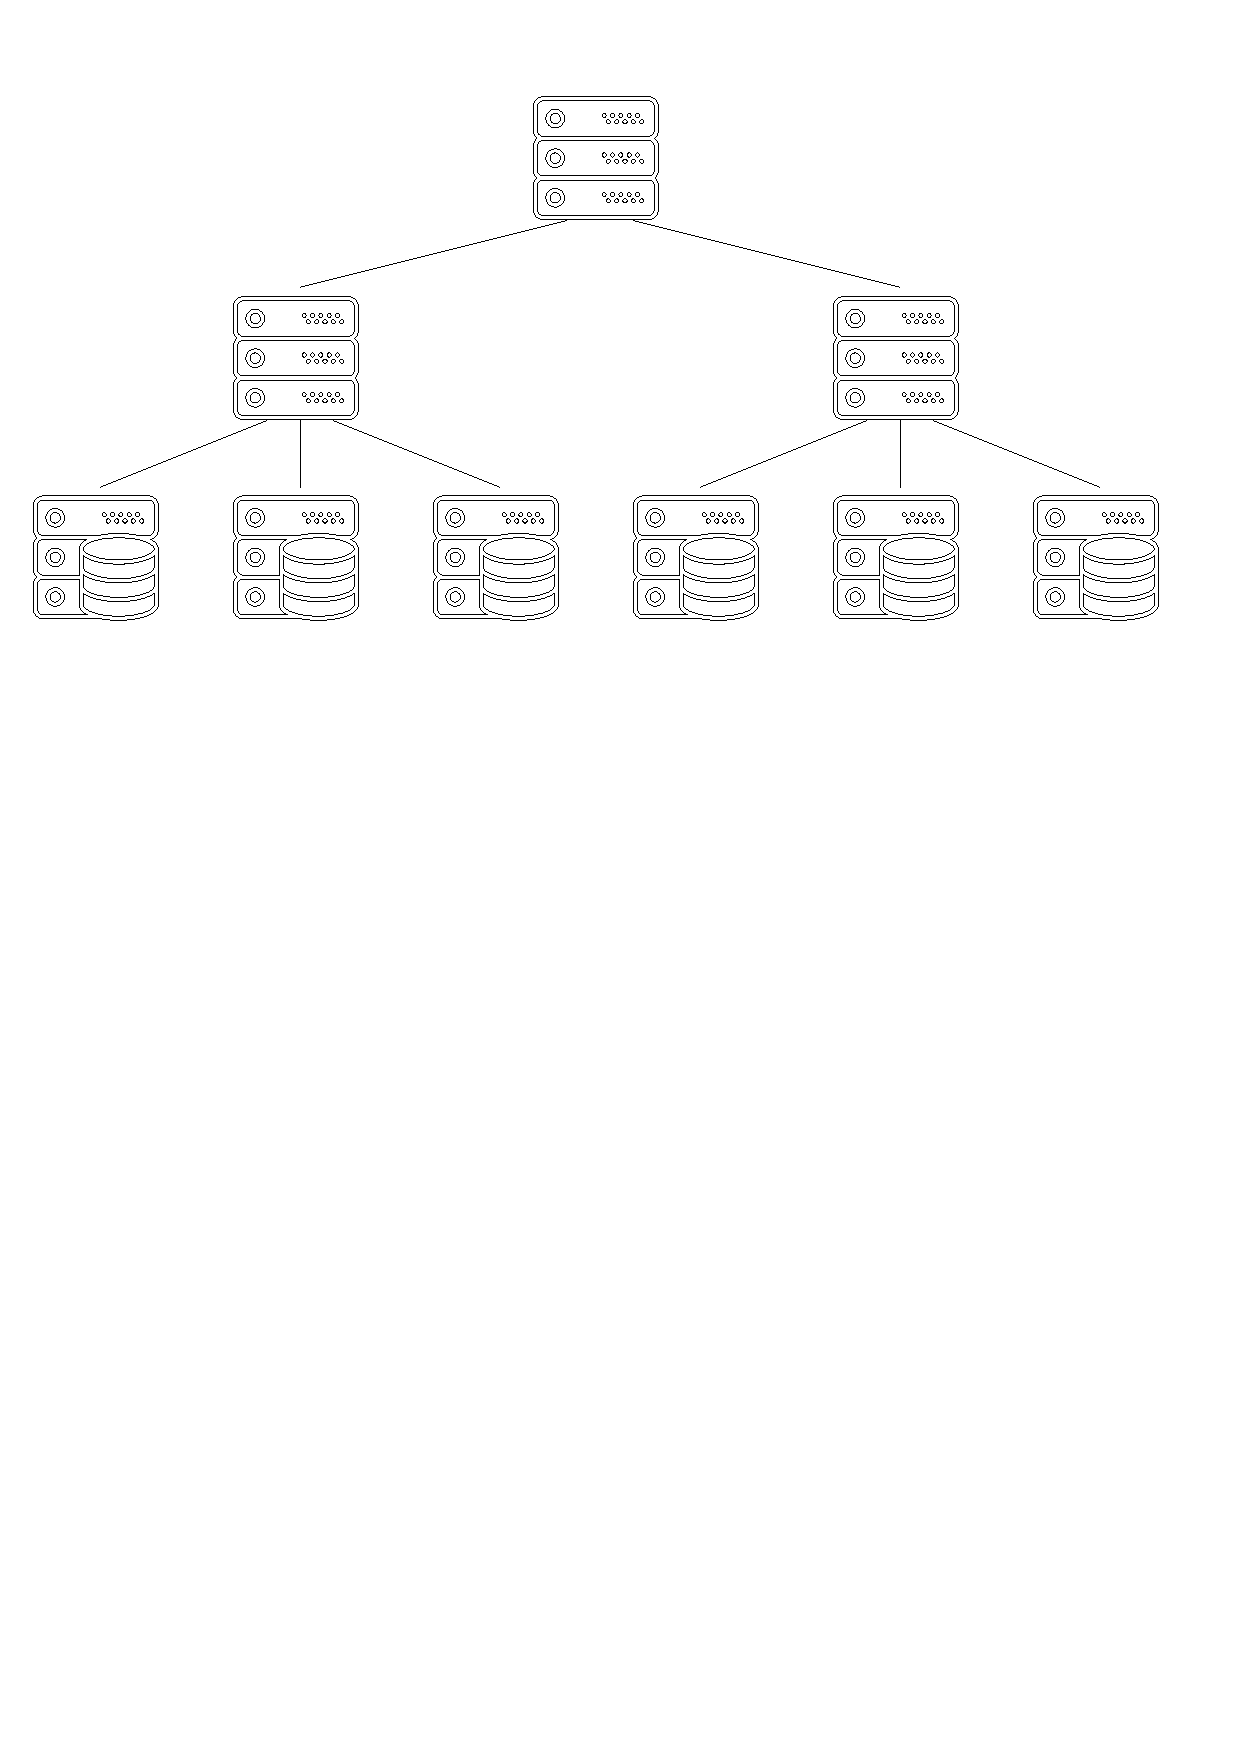
\includegraphics[width=0.79\columnwidth]{figs/tree-topology.pdf}
\caption{The model of typical data center with a tree-like network topology. We distinguish two types of tree nodes: the the intermediate nodes that transmit communication, and the computing machines, located at the leaves of a tree. Network links between nodes are depicted as solid lines.}\label{fig:tree-topology}
\vspace{-1em}
\end{figure}


\subsection{Our Contributions}

We consider two scenarios regarding virtual network embeddings:
\begin{enumerate}
  \item \emph{The static scenario}, where virtual machines are irrevocably assigned to their physical machines.
  \item \emph{The dynamic scenario}, where virtual machines can migrate between physical machines.
\end{enumerate}

We investigate the static scenario in Chapter~\ref{ch:static-mapping}, and the dynamic scenario in Chapter~\ref{ch:dynamic-mapping}.
Although the problems are related by their practical motivations, their combinatorial structure differs substantially.
In particular, the static scenario is not an offline version of the problem considered in the dynamic scenario.
In both scenarios, we assume that the communication pattern among virtual nodes is not known in advance.
In the static scenario we reserve a~portion of a~bandwidth between every pair of virtual nodes to allow for any possible communication pattern.
On the other hand, in the dynamic scenario we react to changes in the communication pattern by migrating machines on the fly.
In addition, the problem considered in the static scenario is enriched by certain important properties of batch-processing applications that use distributed file systems.


\subsubsection{Static Mapping of Virtual Networks}
\label{sec:contributions-static-mapping}

In the static scenario studied in Chapter~\ref{ch:static-mapping}, to guarantee certain quality of service (\emph{QoS}), we need to acquire network reservations for all pairs of cooperating virtual machines.
The combinatorial problem that we consider in the static scenario is essentially a variant of the minimum-cost embedding of a clique (the communication graph) in a tree (the substrate network).
In addition, the scenario is designed to model certain aspects of MapReduce~\cite{mapreduce}, which is a predominant framework for performing large-scale parallel data processing.
We consider the wide range of possible extensions that model certain aspects of Map-Reduce applications, most notably:

\begin{itemize}
\item \emph{Data chunk processing}. In Map-Reduce applications, virtual machines process large amounts of data chunks that are stored in a distributed file system. Each chunk of data must be assigned and transferred to a virtual machine. Data chunk transfer requires its own network reservations.

\item \emph{Data chunk replication}. Distributed file systems often store redundant copies of data chunks, called \emph{chunk replicas}. Only one copy of each data chunk replica must be processed, and we are free to choose the replica to be used based on its placement.

\item \emph{Bandwidth constraints}. Each link in substrate network has its capacity. For the embedding to be feasible, the total network reservations has to obey link capacities.
\end{itemize}


In particular, we decompose the general optimization problem into its fundamental aspects, such as
assignment of chunks, replica selection, and flexible virtual machine
placement, and answer questions such as:
\begin{itemize}
\item Which chunks to assign to which virtual machine?

\item How to exploit redundancy and select good replicas?

\item How to efficiently embed virtual machines and their inter-connecting network?

\end{itemize}

We draw a complete picture of the problem space: we show that
some problem variants (also those exhibiting multiple degrees of freedom in terms of
replica selection and embedding),
can be solved in polynomial time. For all other variants, we prove limitations of their
computational tractability, by proving their NP-completeness. Interestingly,
our hardness results also hold in \emph{uncapacitated}
networks of small-diameter networks (as they are
widely used today~\cite{fattree}).


\subsubsection{Dynamic Mapping of Virtual Networks}
\label{sec:contributions-dynamic-mapping}

In Chapter~\ref{ch:dynamic-mapping}, we study virtual network embeddings in the scenario where virtual machines can be migrated during runtime to another physical machine.
Possibility of migration provides efficient tools that allow to react to unpredictible communication patterns.
For example, if some distant nodes communicate often, it is vital to reduce the distance to save network bandwidth.
The objective is to minimize the total network bandwidth used for communication and for migration.

We assume that the communication patterns are not known in advance.
We measure the quality of presented algorithmic solutions by competitive analysis~\cite{borodin-book}, which is well-suited for problems that are online by their nature.
In competitive analysis, the goal is to optimize \emph{the competitive ratio} of a given online algorithm by comparing its performance to an optimal offline algorithm that is provided with the whole input sequence in advance.
To obtain the competitive ratio for a minimization problem, we take the minimum (over any input sequence) of the cost of an online algorithm divided by the cost of an offline algorithm.

In the dynamic scenario, we assume that the physical substrate network takes a form of a~tree with height one.
Every physical machine (leaf) is connected directly to the root (that has no virtual machine hosting capabilities).
A single physical machine hosts a fixed number of virtual machines.

The model restricted to such networks becomes a variant of online graph clustering.
That is, we are given a~set of~$n$ nodes (virtual machines) with time-varying pairwise
communication patterns, which have to be partitioned into~$\ell$~clusters (physical machines) of
equal size~$k=n/\ell$.

Intuitively, we would like to minimize inter-cluster
interactions by mapping frequently communicating nodes to the same cluster.
Since communication patterns change over time, partitions should be
readjusted dynamically, that is, the nodes should be \emph{repartitioned}, in
an online manner, by \emph{migrating} them between clusters.
The objective is to minimize the weighted sum of inter-cluster communication and repartition costs.
The inter-cluster communication is defined as the number of communication requests between nodes placed in distinct clusters, and the repartition cost is defined as the number of times nodes are migrated from one cluster to
another.


The possibility to perform a migration uncovers algorithmic challenges:
\begin{itemize}

\item \emph{Serve remotely or migrate?} For a brief communication
pattern, it may not be worthwhile to collocate the nodes: the migration cost might
be too large in comparison to communication costs.

\item \emph{Where to migrate, and what?}
If an algorithm decides to collocate nodes $x$ and~$y$, the question becomes
how. Should $x$ be migrated to the cluster holding $y$, $y$ to the one holding
$x$, or should both nodes be migrated to a new cluster?

\item \emph{Which nodes to evict?}
There may not exist sufficient space in the desired destination cluster. In
this case, the~algorithm needs to decide which nodes to ``evict'' (migrate to
other clusters), to free up space.

\end{itemize}

In the considered model, every physical machine fully utilizes its processing capabilities --- it hosts maximum possible amount of virtual machines, i.e. $k=n/\ell$.
Hence, the migration is not possible without the further reconfigurations: to respect physical machine capacity, we need to decide which virtual machines to swap.
For this setting, we show deterministic lower bound of $k$, where $k$ is the physical machines hosting capacity.
We present constant-competitive algorithm for the scenario restricted to physical machines that host two virtual machines ($k = 2$).

In Chapter~\ref{ch:dynamic-mapping}, we also consider the resource-augmentated scenario, where we relax this assumption: the total hosting capacity of physical machines exceeds the total number of virtual machines, i.e. $k > n/\ell$.
Surprisingly, the lower bound remains $k$ also in this setting.
The main contribution of this part is an $O(k\cdot \log(k))$-competitive algorithm for the scenario with small resource augmentation.

%This fundamental online optimization problem has many applications. For
%example, in the context of~cloud computing, $n$ may represent virtual machines
%or containers that are distributed across~$\ell$ physical servers, each having
%$k$ cores: each server can host $k$ virtual machines. We would like to
%(dynamically) distribute the virtual machines across the servers such that
%datacenter traffic and migration costs are minimized.


\subsection{Related Work}


Recently, there has been much interest in programming models and distributed
system architectures for the processing and analysis of big data (see e.g.,~\cite{nodb,mapreduce,shark}).
Such applications
generate large amounts of network traffic~\cite{orchestra,talk-about,amazonbw},
and over the last years, several systems have been proposed which provide
a provable network performance, also in shared cloud environments, by supporting
relative~\cite{faircloud,elasticswitch,seawall}
or, as in the case of this thesis, \emph{absolute}~\cite{oktopus,secondnet,drl,gatekeeper,proteus} bandwidth reservations
between the virtual machines.

In Chapter~\ref{ch:static-mapping}, we study static virtual network embeddings.
Our model is enriched by motivations that follow from batch-processing applications~\cite{mapreduce}.
The most popular virtual network abstraction for such applications today is the \emph{virtual cluster}~\cite{oktopus}, later studied by many others~\cite{talk-about,infocom16,ccr15emb,proteus}.
From a theoretical perspective, the virtual network embedding problem can be seen as a generalization
of classic VPN graph embedding problems~\cite{Goyal2008,gupta2001provisioning}. VPN problem requires finding a graph embedding with fixed endpoints, while in virtual network embedding problems studied in this thesis, the embedding endpoints are subject to optimization.
In this respect, the virtual network embedding problem can also be seen as related to
classic Minimum Linear Arrangement problem~\cite{mla-schmoys} which asks for the
embedding of guest graphs on a simple \emph{line topology} (rather than tree-like topologies as
studied in this thesis).

In Chapter~\ref{ch:dynamic-mapping}, we study an online balanced partition problem.
The static offline version of the problem, i.e., a problem variant where
migration is not allowed, where all requests are known in advance, and where
the goal is to find best node assignment to $\ell$~clusters, is known as the
\emph{$\ell$-balanced graph partitioning problem}. The problem is 
NP-complete, and cannot even be approximated within any finite factor unless P
= NP~\cite{AndRae06}.  The static
variant where $\ell = 2$ corresponds to the minimum bisection problem, which
is already NP-hard~\cite{GaJoSt76}.
Its approximation was studied in a long
line of work~\cite{SarVaz95,ArKaKa99,FeKrNi00,FeiKra02,KraFei06,Raec08} and
the currently best approximation ratio of $O(\log n)$ was given by
R{\"{a}}cke~\cite{Raec08}.
The inaproximability of the static variant for general values of $\ell$
motivated research on the bicriteria variant, which can be seen as the offline
counterpart of our cluster-size augmentation approach. Here, the~goal
is~to~develop $(\ell,\delta)$-balanced graph partitioning, where the graph has
to be partitioned into $\ell$ components of~size less than $\delta \cdot (n /
\ell)$ and the cost of the cut is compared to the optimal (non-augmented)
solution where all components are of size~$n / \ell$. The variant where
$\delta \geq 2$ was considered in
\cite{LeMaTr90,SimTen97,EvNaRS00,EvNaRS99,KrNaSc09}. So far, the best result is
an $O(\!\sqrt{\log n \cdot \log \ell})$-approximation by Krauthgamer et
al.~\cite{KrNaSc09}, which builds on ideas from the $O(\!\sqrt{\log
n})$-approximation algorithm for balanced cuts by Arora et al.~\cite{ArRaVa09}.

Our model is related to online
paging~\cite{SleTar85,FKLMSY91,McGSle91,AcChNo00}, sometimes also referred to
as online caching, where requests for data items (nodes) arrive over time and
need to be served from a cache of finite capacity, and where the number of
cache misses must be minimized. Classic problem variants usually boil down to
finding a smart eviction strategy, such as Least Recently Used (LRU). In our
setting, requests can be served remotely (i.e., without fetching the
corresponding nodes to a single cluster). In this light, our model is more
reminiscent of caching models \emph{with
bypassing}~\cite{EpImLN11,EpImLN15,Irani02}. As a side result, we show that our problem is
capable of emulating online paging.

There is a major difference between the dynamic embedding problem and the caching problems.
These problems typically maintain some configuration of servers or
bought infrastructure and upon a new request (whose cost typically depends on
the distance to the infrastructure), decide about its reconfiguration (e.g.,
server movement or purchasing additional links). In contrast, in our model,
\emph{both} end-points of a communication request are subject to optimization.



\section{Router Memory Optimization}
\label{sec:intro-packet-forwarding}

\subsection{Forwarding Rules}

In the second part of this thesis, we consider the fundamental problem of \emph{packet forwarding}.
We focus on a single router, that physically connects different networks and is responsible for passing packets between them.
Upon receiving a data packet, the router forwards it to a~specific output port leading to a neighbouring network.
To choose the appropriate port, the router stores of a \emph{forwarding table}, which consists of rules describing how to map the packet destination addresses to appropriate ports.

Certain routers (e.g. in Internet exchange points) are located near the core of the Internet, and forward packets among large number of networks.
Hence, their forwarding tables usually contain forwarding entries for all of them.
In Figure~\ref{fig:bgp-entries}, we see the growth of the number of entries in the global forwarding table \cite{url-bgp-entries}.
Size of forwarding tables of the routers in the core of the Internet are approaching such size.
Those routers have to store an~enormous number of forwarding rules: the
number of rules has doubled in the last six years~\cite{bgp-routeviews} and
the superlinear growth is likely to be sustained~\cite{steve-myth}.

It is worth noting that networks can be either physical or virtual.
The concept of virtual networks described in Part~\ref{pt:virtual-networks} contributes immensely to partition of the Internet into subnetworks, and to growth of forwarding tables.


The router maintains the forwarding table in its memory.
Only a small restricted set of operations is performed on such memory: lookups and updates.
Nowadays, routers perform milions of lookup operations and thousands updates (see, e.g. a raport~\cite{bgp-updates}), and the utilizing specialized hardware is crucial for the efficiency of packet forwarding.
Hence, instead of relying on the general-purpose memory such as RAM (where lookup operation is costly), the specialized memory units such as TCAM~\cite{tcam-memory} are utilized.
The TCAM memory is an associative memory storage with a variation of pattern-matching lookup that closely matches the way the forwarding rules are used.

With the growth of the Internet, the number of connected networks increases with rapid progression, which often induces new forwarding rules to store.
In effect, the size of forwarding table exceeds the amount of available TCAM memory in a typical router (the phenomenon called the TCAM exhaustion~\cite{tcam-exhaust}).
Sophisticated electronics circuits such as TCAM are very expensive and power-hungry~\cite{tcam-expensive} in comparison to RAM.
Moreover, typical operations performed on TCAM memory examine the whole contents stored in memory, which requires closely connected physical structure among memory cells --- as the result, it is expensive to expand available memory.

Limited size of memory and expanding size of the content to store brings new challenges in memory management of the routers.
In the second part of this thesis, we investigate the following problem, using the tools provided by contemporary routers:
\begin{center}
  \emph{How to efficiently manage the memory of forwarding devices?}
\end{center}

In this thesis, we investigate the scenario, where we store only the subset of forwarding rules in fast TCAM memory.
If the forwarding rule is not present, we perform a query to slower (possibly remote) memory.
Although this setting resemble the caching problem, the hierarchical structure of forwarding rules enforces some restrictions of cache configuration feasibility.
Forwarding rules form a tree, and the child rule describes the exception to the parent rule.
Hence, to preserve the semantics of the forwarding rules set, no parent rule can be in cache without its child rules.
In other words, every valid cache configuration is a bottom-contignous subforest.
We elaborate more in Chapter~\ref{ch:cache-management}.


\begin{figure}[t]
\centering
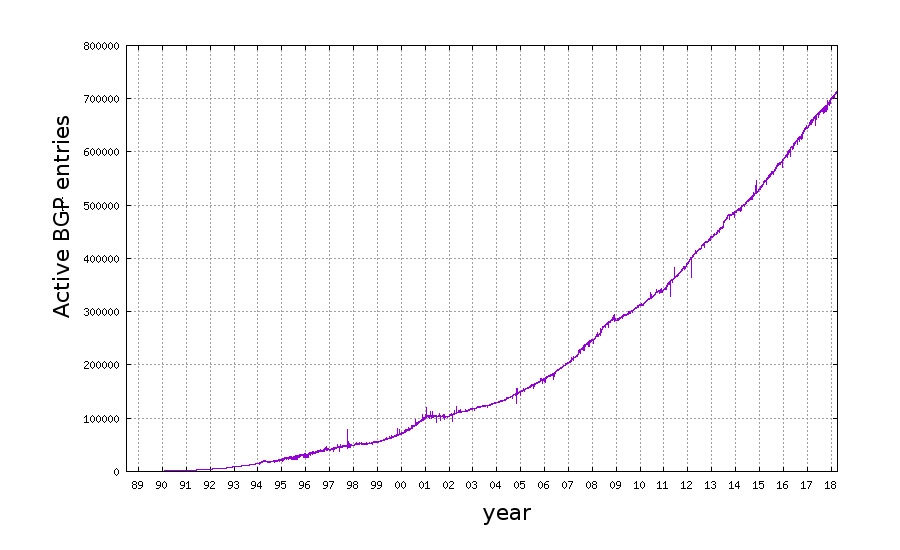
\includegraphics[width=0.59\columnwidth]{figs/bgp-entries.png}
\caption{The number of entries in the global forwarding table. The global forwarding table is built upon the informations exchanged via Border Gateway Protocol. The graph presents the growth of the global forwarding table from 1988 to 2018.}\label{fig:bgp-entries}
\end{figure}

\subsection{Our Contributions}

We initiate the study of a natural new caching with bypassing problem which
allows to account for tree-dependencies among items.
We present a deterministic online
algorithm~\ALG for the Tree Caching problem. While our algorithm is simple, its analysis
 requires several non-trivial
insights into the problem. In particular, we rigorously prove that \ALG is
$O(h(T)\cdot k)$-competitive, where $h(T)$ is the height of tree~$T$, and $k$ is the size of available cache.
Note that this
result is optimal up to the factor~$O(h(T))$: we show that the lower
bound~$R$ for the paging problem~\cite{competitive-analysis} implies an
$\Omega(R)$ lower bound for our problem for any $\alpha \geq 1$. Finally, we show that \ALG can be
implemented efficiently.

In addition, we consider the online tree caching problem within the resource
augmentation paradigm: we assume that cache sizes of the online algorithm
($\kALG$)  and the optimal offline algorithm ($\kOPT$) may differ. We assume
$\kALG \geq \kOPT$ and let $R = \kALG/(\kALG-\kOPT+1)$.
For this setting we show that \ALG is
$O(h(T) \cdot R)$-competitive.



\subsection{Related Work}

So far, the papers on IP rule caching avoided dependencies either assuming
that rules do not overlap (a~tree has a single level)~\cite{route-caching-flat} 
or by preprocessing the tree, so that the rules become
non-overlapping~\cite{prefix-caching,fib-caching-non-overlapping}.
Unfortunately, this could lead to a large inflation of the routing table. A
notable exception is a recent solution called CacheFlow~\cite{cacheflow}. The
CacheFlow model supports dependencies even in the form of directed acyclic
graphs. However, CacheFlow was evaluated only experimentally, and no
worst-case guarantees were given on the overall cost of caching. Our work
provides theoretical foundations for respecting tree dependencies.


Other approaches for minimizing the number of stored rules were mostly based
on \emph{rules compression (aggregation)}, where the set of rules was replaced
by another equivalent and smaller set. Optimal aggregation of a fixed routing
table can be achieved by dynamic
programming~\cite{ortc,fib-compression-two-dimensional}, but the main
challenge lies in balancing the achieved compression and the amount of changes
to the routing table in the presence of \emph{updates} to this table. While
many practical heuristics have been devised by the networking community for
this problem~\cite{mms,fib-compression-fifa,fib-compression-globecom10,fib-compression-infocom13,fib-sigcomm,fib-compression-smalta,fib-compression-infocom10},
worst-case analyses were presented only for some restricted
scenarios~\cite{fib-icdcs,fib-sirocco}. Combining rules compression and rules
caching is so far an unexplored area.



\section{Bibliographic notes and acknowledgements}

The results of this thesis were published by the author of this thesis in various conferences and journals.
Parts of Chapter~\ref{ch:static-mapping} appeared previously in the proceedings of 23rd IEEE International Conference on Network Protocols (ICNP 2015)~\cite{my-icnp},
and in Theoretical Computer Science, vol.~697~\cite{my-tcs}.
Some of the results from Chapter~\ref{ch:static-mapping} appeared in the PhD thesis of my co-author Carlo Fuerst.
Parts of Chapter~\ref{ch:dynamic-mapping} appeared previously in the proceedings of 30th International Symposium on Distributed Computing (DISC 2016)~\cite{my-disc}, and parts of Chapter~\ref{ch:packet-forwarding} --- in the proceedings of 29th ACM Symposium on Parallelism in Algorithmics and Architectures (ACM~SPAA~2017)~\cite{my-spaa}.
Preliminary results from Chapter~\ref{ch:packet-forwarding} appeared in the master thesis of my co-author Aleksandra Spyra.

For some figures in this thesis, icons by Smashicons from www.flaticons.com were used.

\part{Mapping virtual networks}

Common introduction to chapters 1 and 2. I think that this part does not require separate chapter.


References and comparisons from chapter 2 to chapter 1:
\begin{enumerate}
  \item Make a clear connection to embedding from the previous chapter.
  \item Dynamic = discovering the structure of the object to embed in online fashion.
  \item Similar objective function: bandwidth reservation upfront and charging for the communication
  \item Virtual cluster = the worst case bandwidth reservation (complete graph) with KNOWN size; Virtual Cluster $\rightarrow$ data locality and replica selection part of the problem
  \item The extension of the model: migrations that take bandwith reservation (or communication cost) of certain size $\alpha$
\end{enumerate}
Problems that arise (in paper: part of the model): rent or buy / where to migrate and what / which nodes to evict



\chapter{Virtual networks with static topology}


For executing a certain computation, one places an adequate number of workers, whose task is to select their data portion, process them, and aggregate the result by cooperation with other workers.
Workers establish a network connection called a virtual network, formed to peform a~given computational task, and in such setting the worker is referred to as a node of a virtual network.
While these nodes can be placed at~any feasible physical machine in the data center, the processing performance processing is heavily influenced by their placement.
Placing nodes closely to each other reduces network latency and bandwidth reservations in the data center.
In this chapter, we investigate mapping a virtual network onto the physical infrastructure: a~task of~assigning the nodes of a virtual network to~physical machines in a network-efficient way.

\section{Problem Definition}\label{sec:model}

As described informally in the introduction (see Section~\ref{sec:virt_net_emb}), the model combines three components: (1)~the~substrate network (the servers
and the connecting physical network),
(2)~the virtual network (the virtual machines and the logical network connecting the machines to each other
as well as to the data), and (3)~the data divided into data chunks that needs to be processed.
For the remainder of this chapter, we restrict our attention to the substrate networks that form a tree, and a particular virtual network topology, called the virtual cluster, which is basically a fully connected graph (a clique).
We~refer to aforementioned problem as the \textsc{cluster-in-tree embedding} problem, abbreviated \CTE.
Below we provide the details of components of \CTE. Figure~\ref{fig:overview} gives an overview of our model.


\parag{The Substrate Network.} The substrate network (also known as the \emph{host graph}) represents the physical resources:
a~set~$S$ of~$n_S=|S|$ servers inter-connected by a network consisting of a~set~$R$ of routers (or switches)
and a~set~$E$ of (symmetric) links. We often refer to the elements in~$S\cup R$
as the \emph{vertices}. We assume that the inter-connecting network forms an arbitrary rooted tree $T$,
where the servers are located at the tree leaves and routers at inner nodes.
Depending on the available capacity~$\capacity(s)$ of server~$s$, multiple virtual machines may be hosted on~$s$.
Each link~$e\in E$ in the substrate network has a certain bandwidth capacity~$\capacity(e)$.

\parag{The Data.} The data to be processed constitutes the input to the batch-processing application.
The data is stored in a distributed filesystem spread across the servers; this spatial distribution is given and is not subject to optimization.
The input data consists of~$\tau$ different \emph{chunks}~$\achunk_1, \ldots, \achunk_{\ChunkType}$,
where each chunk~$\achunk_i$ can have~$r_i\geq 1$ instances (replicas)~$\achunk_{i}^{(1)},\ldots, \achunk_{i}^{(r_i)}$,
 stored at different servers. A single server may host multiple chunks.
It is sufficient to process one replica of each chunk, and we refer to this
replica as the \emph{active} (or selected) replica.

\parag{The Virtual Network.} The virtual network $\VirtualNodes$ consists of $n_V=|\VirtualNodes|$ virtual machines, called \emph{nodes}.
Each node can be placed (or, synonymously, embedded) on an arbitrary server and this placement is subject
to optimization.
Furthermore, to enable nodes to process the data, we provide the virtual network with network connections.
The \emph{(node) inter-connect network} forms a~complete network (a clique) among nodes,
and the \emph{(chunk) access network} consists of links from each active replica to the node that is assigned to process it.
In order to ensure a predictable application performance, both these networks require certain minimal bandwidth guarantees.
Concretely, we assume that each chunk
is connected to its processing node at a~bandwidth~$\CostTrans$, and each node is connected to any other node
at  bandwidth~$\CostCom$.
The choice of replica and processing node is subject to optimization, and
$\mu$ denotes the assignment of chunks to nodes.
Furthermore, we assume that the number of chunks $\tau$ is divisible by the number of nodes~$n_V$, and the assignment~$\mu$ is \emph{balanced}:
each node processes exactly $\tau / n_V$ chunks.
Collectively, the nodes of virtual network with the inter-connect network and the access network form the \emph{virtual cluster}.
Note that our definition extends the notion of the virtual cluster studied by others \cite{oktopus,talk-about,infocom16,ccr15emb,proteus} by incorporating the chunk access network.


\begin{figure}[t]
\centering
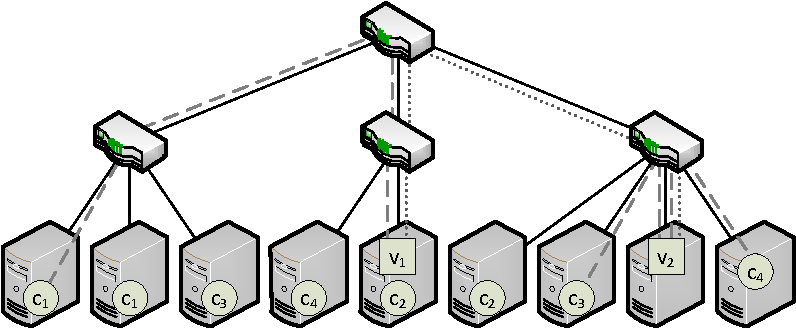
\includegraphics[width=0.79\columnwidth]{figs/static-mapping/data_locality_no_legend.pdf}
\caption{Overview: a 9-server datacenter storing~$\tau=4$ different chunks~$\{c_1,\ldots,c_4\}$ (depicted as \emph{circles}), each having two replicas. The replicas need to be selected and assigned to the two
 virtual machines~$v_1$ and~$v_2$; the virtual machines are depicted as \emph{squares}, and
 the network connecting them to chunks (using bandwidth~$\CostTrans$) is \emph{dashed}. In addition, the virtual machines are inter-connected among
 each other using bandwidth~$\CostCom$ (\emph{dotted}). The objective of the embedding algorithm is to minimize the overall bandwidth allocation.}\label{fig:overview}
\end{figure}


\parag{Optimization Objective.} 
Our goal is to design algoriths that minimize the resource \emph{footprint}, the most common objective function considered in the literature \cite{fischer-survey}.
Formally, let~$\dist(v,\achunk)$ denote the~distance (in the underlying physical network~$\Tree$) between a~node~$v$ and
its assigned (active) replica~$\achunk$, and let~$\dist(v_1,v_2)$ denote the distance between the two nodes~$v_1$ and~$v_2$.
We define the \emph{footprint}~$\Cost(v)$ of a node~$v$ as follows:
$$
\Cost(v) = \underbrace{\sum_{\achunk \mid \mu(c) = v} \CostTrans \cdot \dist(v,\achunk)}_{\text{chunk access cost}} +  \underbrace{\frac{1}{2} \cdot \sum_{v' \in \VirtualNodes\setminus\{v\}} \CostCom \cdot \dist(v,v')}_{\text{node inter-connect cost}},
$$
where~$\mu(c)$ is the node to which chunk $c$ is assigned.
Our goal is to minimize the overall resource footprint $\Cost=\sum_{v\in V} \Cost(v)$.
The solution must obey the capacity of the substrate network: (1)~the total number of nodes hosted at each server $s$ must not exceed $\capacity(s)$, and (2)~the total bandwidth allocated at each link $e$ must not exceed its capacity $\capacity(e)$.
%Finally, the solution must assign every chunk to some node, i.e., $\bigcup_v \mu(v) = \{ c_1, \ldots, c_{\tau} \}$.

\subsection{Problem Decomposition}

We introduced the $\CTE$ problem in its full generality.
To fully chart the algorithmic complexity of $\CTE$, we decompose the problem into its fundamental components that can be activated or deactivated independently of each other, and we consider all possible variants.
Concretely, we consider $5$ aspects of $\CTE$, namely multiple chunk assignment ($\MA$),
replica selection ($\RS$), flexible node placement ($\FP$), node inter-connect ($\NI$),
and bandwidth constraints ($\BW$), as~described below.

\parag{Multiple Assignment ($\MA$).}
In most applications, the number of chunks~$\tau$ is larger than the number of nodes, and the objective is to assign multiple chunks to each node.
In each variant (regardless of $\MA$), we investigate assignments that balances chunks among nodes, i.e., where the number of chunks is divisible by the number of nodes, and each node processes an~identical integer number of chunks.
We require that the number of chunks processed by each node is equal to~$\MaFactor = \tau / n_V$, and we call $\MaFactor$ the multi-assignment factor.
If the number of chunks exceeds the number of nodes, i.e., $\MaFactor > 1$, then we refer to such scenario as $\MA$.
In~the~$\CTE$ variant without $\MA$, each node has exactly one chunk assigned, i.e., $\MaFactor = 1$.

\parag{Replica Selection ($\RS$).}
Distributed filesystems often utilize data redundancy for corruption detection and correction.
A redundant data chunk has multiple \emph{replicas}, stored on different physical machines.
For each data chunk, it is sufficient to process only one of its replicas.
By~$\RS$ we denote the flexibility of choosing which replica of each data chunk to process.
In~the~problem variant without $\RS$, each chunk has a single replica ($r_i = 1$ for all $i$).

\parag{Flexible Placement ($\FP$).}
%In most applications, nodes of virtual network are unconcerned about their physical placement.
By $\FP$ we denote the flexibility of assignment of nodes to~physical machines.
In the problem variant without $\FP$, the assignment of nodes to physical machines is given as an input.

\parag{Node Inter-Connect ($\NI$).}
In some computational tasks, it is sufficient to process data chunks independently of each other.
However, more often the result of processing the individual chunks is combined afterwards.
By $\NI$ we refer to the latter scenario, where the computation requires the nodes to cooperate.
We investigate the scenario, where we reserve a bandwidth of volume $\CostCom$ between each pair of nodes, i.e., the node inter-connect is modelled as a complete graph, to account for the all-to-all communication patterns of batch processing applications such as MapReduce.
In the problem variant without $\NI$, we optimize only the cost of transporting chunks to nodes, and the inter-node communication is set to zero, i.e., $\CostCom = 0$.

\parag{Bandwidth Capacities ($\BW$).}
We distinguish between an uncapacitated and a capacitated scenario where each link $e$
of the substrate network comes with a bandwidth
constraint $\capacity(e)$, and we refer to the bandwidth-constrained version by~$\BW$.
Note that capacity constraints introduce infeasible problem instances, where it is impossible to
allocate sufficient resources to~embed the virtual network.
In the problem variant without $\BW$, each link has infinite capacity, i.e., $\capacity(e) = \infty$ for each edge $e$.

\section{Polynomial-Time Algorithms}\label{sec:poly}


Despite the various degrees of freedom in terms of embedding and replica selection,
we can solve many problem variants efficiently.
 This section introduces three general techniques,
 which can roughly be categorized into
 \emph{flow} (Section~\ref{ssec:flow}), \emph{matching} (Section~\ref{ssec:match}) and \emph{dynamic programming}
 (Section~\ref{ssec:dyn}) approaches.
In Figure~\ref{fig:venn_full}, we either summarize the fastest method to solve the computational problem or its computational intractability.
 
First, let us make a simplifying observation:
\begin{obs}\label{obs:nofp}
In CTE variants without flexible placement (FP),
the bandwidth required
for the inter-connect network (NI) can be allocated upfront, 
as it
does not depend on the replica
selection and the assignment.
Accordingly, we can reduce the variant~$RS+MA+NI+BW$ (as well as all its subproblems)
to~$RS+MA+BW$ (resp.~its subproblems).
\end{obs}

\begin{figure}[t]
\centering
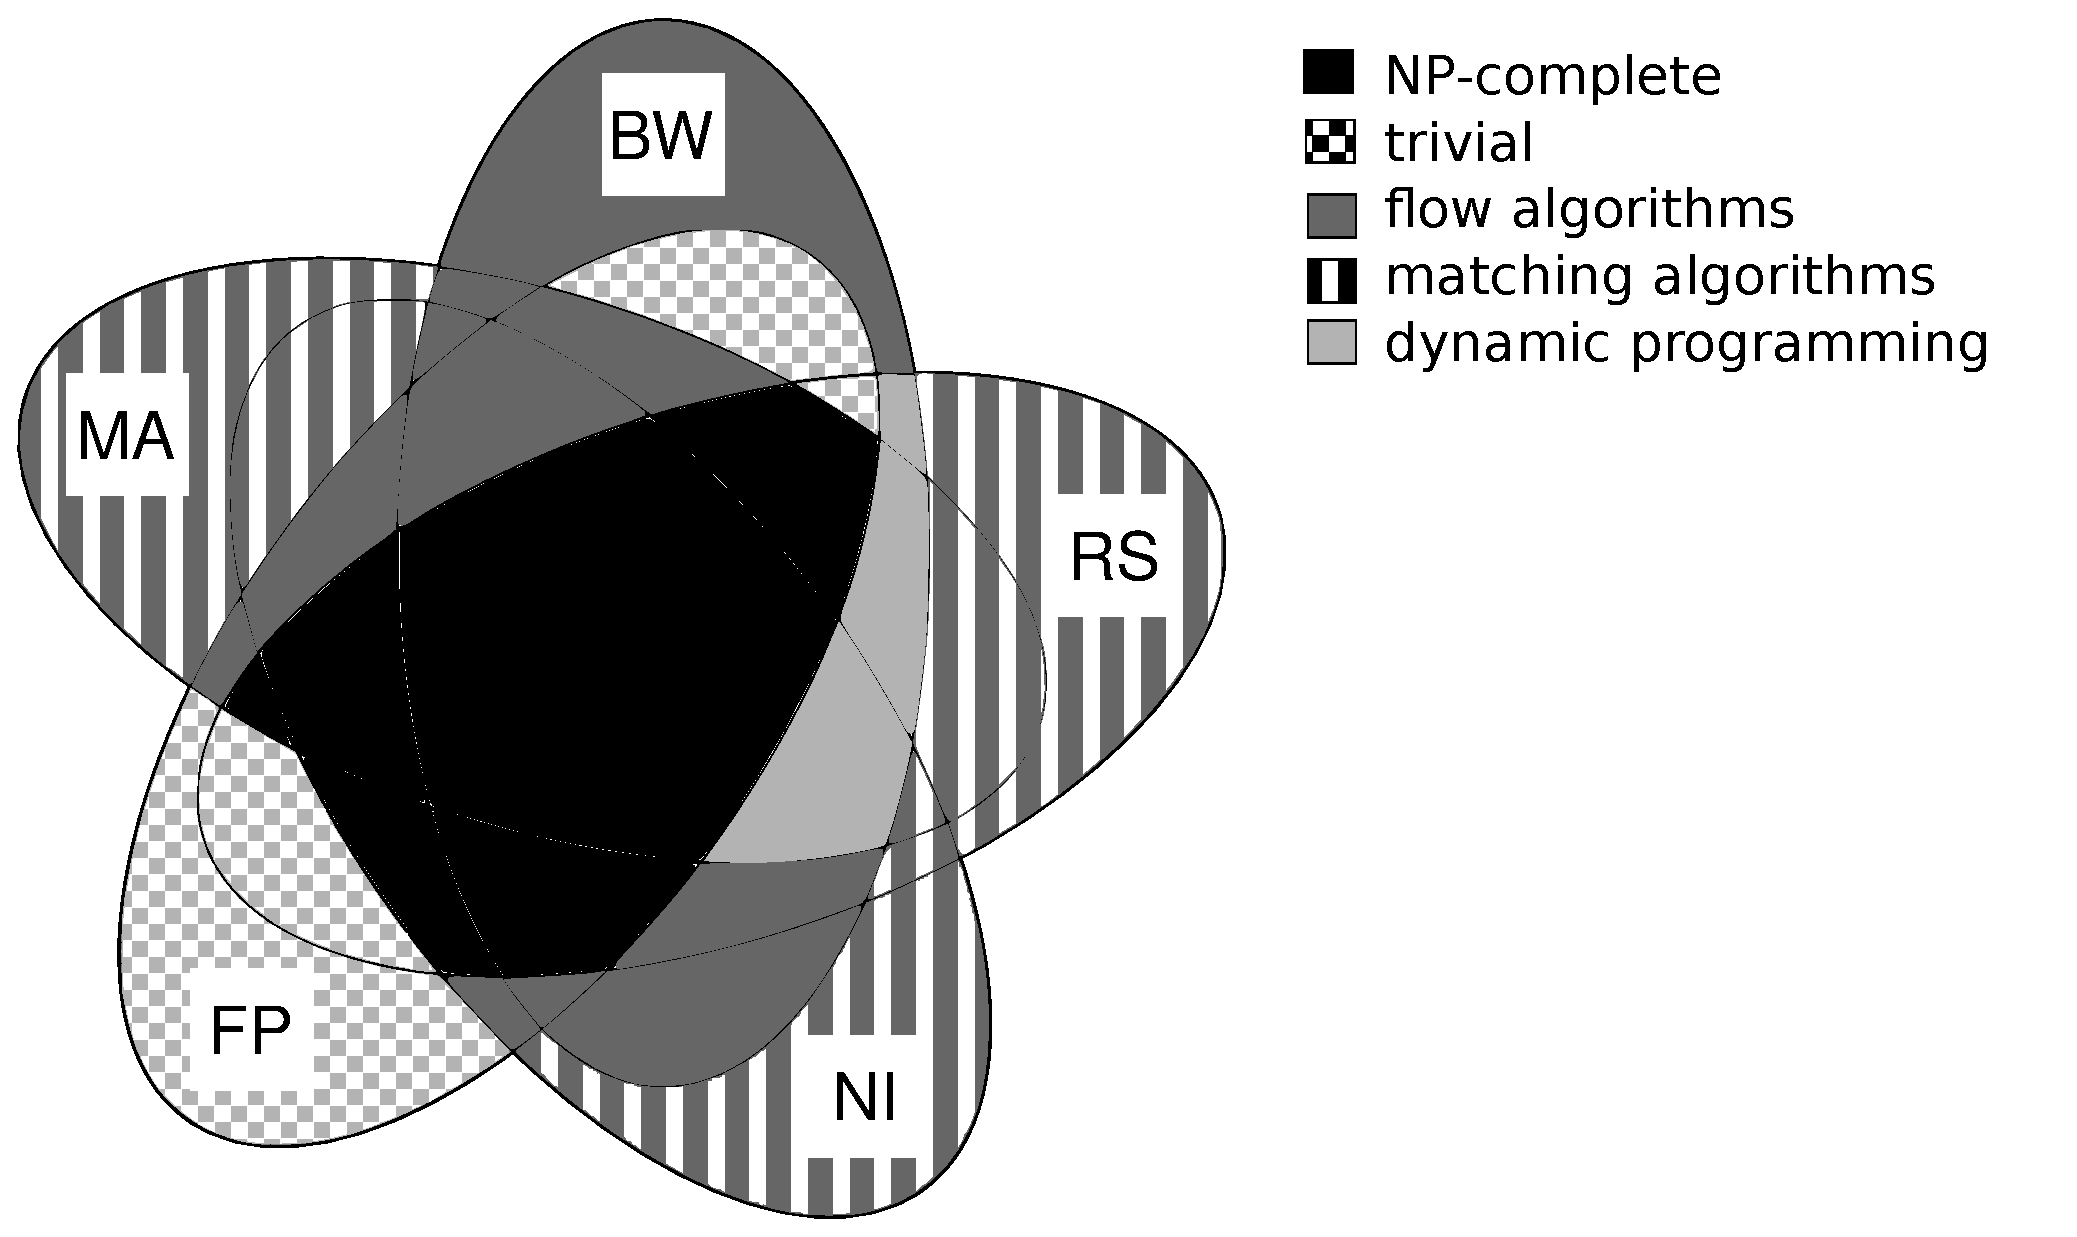
\includegraphics[width=0.69\columnwidth]{figs/static-mapping/venn_full2}
\caption{Fastest algorithms for different respective variants. Variants depicted by solid black are NP-hard, and variants depicted by checked filling are trivially solvable. For the remainder of variants we marked the fastest method.}
\label{fig:venn_full}
\end{figure}


\subsection{Flow-Based Algorithm}\label{ssec:flow}

\begin{figure}
\centering
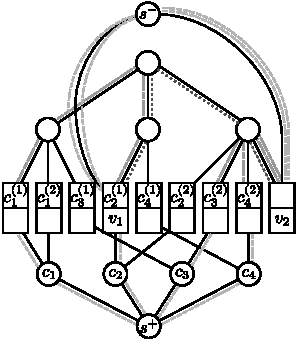
\includegraphics[width=0.5\columnwidth]{figs/static-mapping/flow_ma_cv}
\caption{An example of the extended substrate
network~$\Tree^*$: The sink~$\Sink$ is connected to the two leaves that host the
nodes. The artificial nodes are depicted below the leaves, are labeled with
their respective chunks (e.g.,~$\achunk_1$), and are connected to the source
$\Source$ as well as to the leaves that contain replicas of their chunk.
The~maximum flow with minimum cost is indicated by the dashed lines: each line
represents one unit of flow. The~dotted lines indicate links which have reduced
capacity due to~$\NI$.}
%\caption{Example of flow construction: Problem instance with two nodes, four chunk
%types, and two replicas per type. The min-cost-max-flow
%is indicated by the dashed lines: each line represents one unit of flow.
%}
\label{fig:flow_construction}
\end{figure}



%\begin{figure}[t]
%\centering
%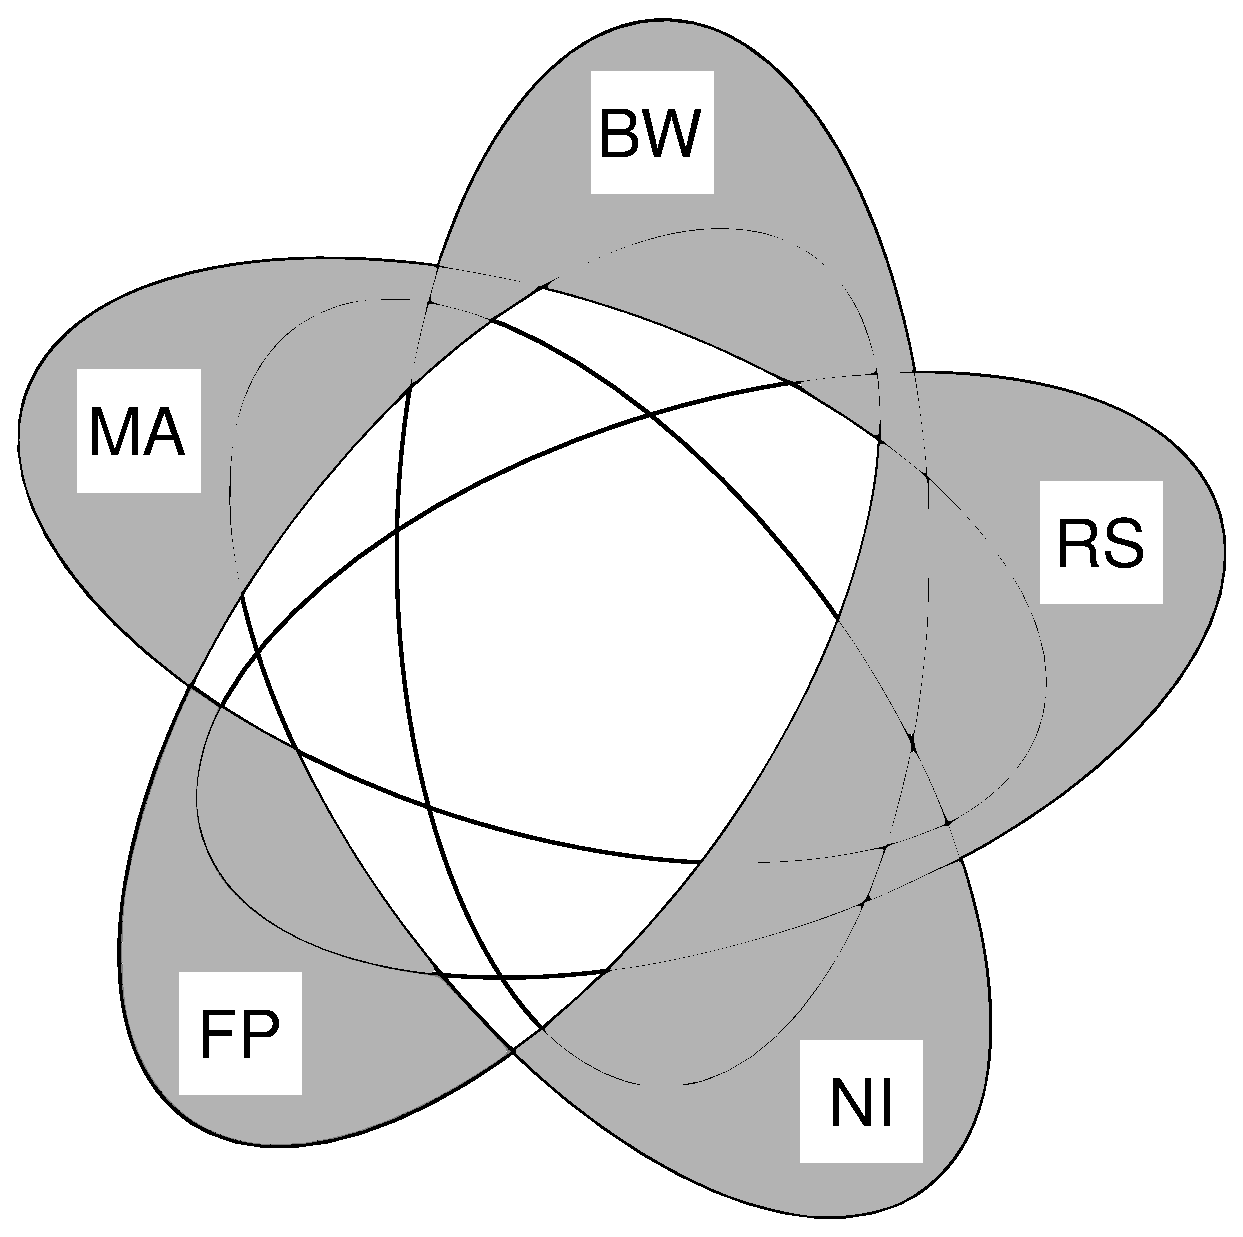
\includegraphics[width=0.49\columnwidth]{figs/static-mapping/venn_flow.pdf}
%\caption{Variants solved by flow approach.}
%\label{fig:venn_flow}
%\end{figure}


We first present an algorithm to solve the~$\RS+\MA+\NI+\BW$ variant of the $\CTE$ problem.
Recall that in this problem variant,
we are given a~set of redundant chunks ($\RS$) and a~set of
nodes
at fixed locations (no~$\FP$). The number of chunks may be larger than the number
of nodes ($\MA$), and each node needs to be connected
to its selected chunks as well as to other nodes ($\NI$), while respecting
capacity constraints ($\BW$).
As we see in the following, we can use a flow approach to solve this
problem variant.


\parag{Construction of the Artificial Graph.}
In order to solve the~$\RS+\MA+\NI+\BW$ variant of the {\CTE} problem,
we first remove the~$\NI$ component using Observation~\ref{obs:nofp}.
Then, we construct
an artificial graph~$\Tree^*$, extending the substrate network~$\Tree$.
We transform bandwidth capacities, so that they correspond to the maximal number of chunks that we can transfer through the link.
Concretely, for each link~$e\in E(\Tree)$, we set its new
capacity in~$\Tree^*$ to~$\lfloor\capacity(e) / \CostTrans\rfloor$.
After this normalization, we extend the topology of~$\Tree$ by
introducing an artificial vertex for each of $\tau$ chunks. Each of these artificial
vertices is connected to each leaf (i.e., server) in~$\Tree$ where a~replica
 of the respective chunk is located,
connecting the replica by a link of capacity~$1$. In
addition, we construct a
\emph{super-source}~$\Source$, and connect it to each of the artificial chunk
vertices with a link of capacity~$1$. Moreover, we construct an artificial \emph{super-sink}~$\Sink$ and
connect it to every leaf containing at least one node; the link capacity represents
the number of nodes this server hosts times the~multi-assignment factor
$\MaFactor$.
We additionally assign the following costs to edges of~$\Tree^*$:
every edge of the original substrate network costs one unit, and all other artificial edges
cost nothing.
A solution to the~$\RS+\MA+\BW$ variant can now be computed
from a~solution to the \emph{min-cost~max-flow} problem between super-source
$\Source$ and
super-sink~$\Sink$ on the artificial graph~$\Tree^*$.
An illustration of this construction is presented in Figure~\ref{fig:flow_construction}.

\parag{Algorithm.}
Our algorithm to solve the~$\RS+\MA+\NI+\BW$ variant consists of three parts:
First, we construct the extended graph~$\Tree^*$
described above and compute
a~min-cost~max-flow solution.
State-of-the-art~min-cost max-flow algorithm is the double scaling algorithm~\cite{mincostmaxflow-state}, which is based on the scaling technique~\cite{mincostmaxflow-1,mincostmaxflow-2}, .

Second, we have to \emph{round} the resulting, possibly fractional flow, to
integer values. Due~to the~\emph{integrality theorem}~\cite{flow-book},
there always exists an optimal integer solution on graphs with integer capacities.
However, min-cost~max-flow algorithms may yield fractional solutions
which need to be rounded to integral solutions (of the same cost)~\cite{electric-flows}.

Third, given an integer min-cost~max-flow solution, we need to decompose
the integer flow into the paths
representing matched chunk-node pairs:
The assignment can be obtained by decomposing the flow allocated in the
original substrate network. In order to identify a matched chunk-node pair,
we take an~arbitrary (loop-free) path~$p$ carrying a flow of value at least~$1$ from~$\Source$ to~$\Sink$:
the first hop represents the chosen chunk, the second hop the chosen
replica, and the penultimate hop represents the server: we assign
the replica to an arbitrary node on this server that has less than $\MaFactor$ chunks assigned.
Having found this pair, we reduce the flow
along the path~$p$ by one unit.
We continue the pairing process until every chunk is assigned.

\parag{Analysis.}
The runtime of our algorithm consists of four parts: construction of~$\Tree^*$,
computation of the min-cost~max-flow, flow rounding, and decomposition. The
dominant term in the~asymptotic runtime is the flow computation.
Using the double scaling algorithm for min-cost~max-flow~\cite{mincostmaxflow-state}, we get a runtime of~$\mathcal{O}(|E|^2 \cdot\log\log U \cdot \log |E|)$
where~$|E| = n_S+\sum_{i=1}^\tau r_i + n_V$ is the number of $\Tree^*$ edges, and~$U$ is the maximal link capacity. Note that in networks with high capacity
and uncapacitated networks, we can simply set~$U=\tau$, so the resulting overall runtime is $\mathcal{O}(|E|^2 \cdot\log\log \tau \cdot \log |E|)$.


\subsection{Matching Algorithms}\label{ssec:match}


%\begin{figure}[t]
%\centering
%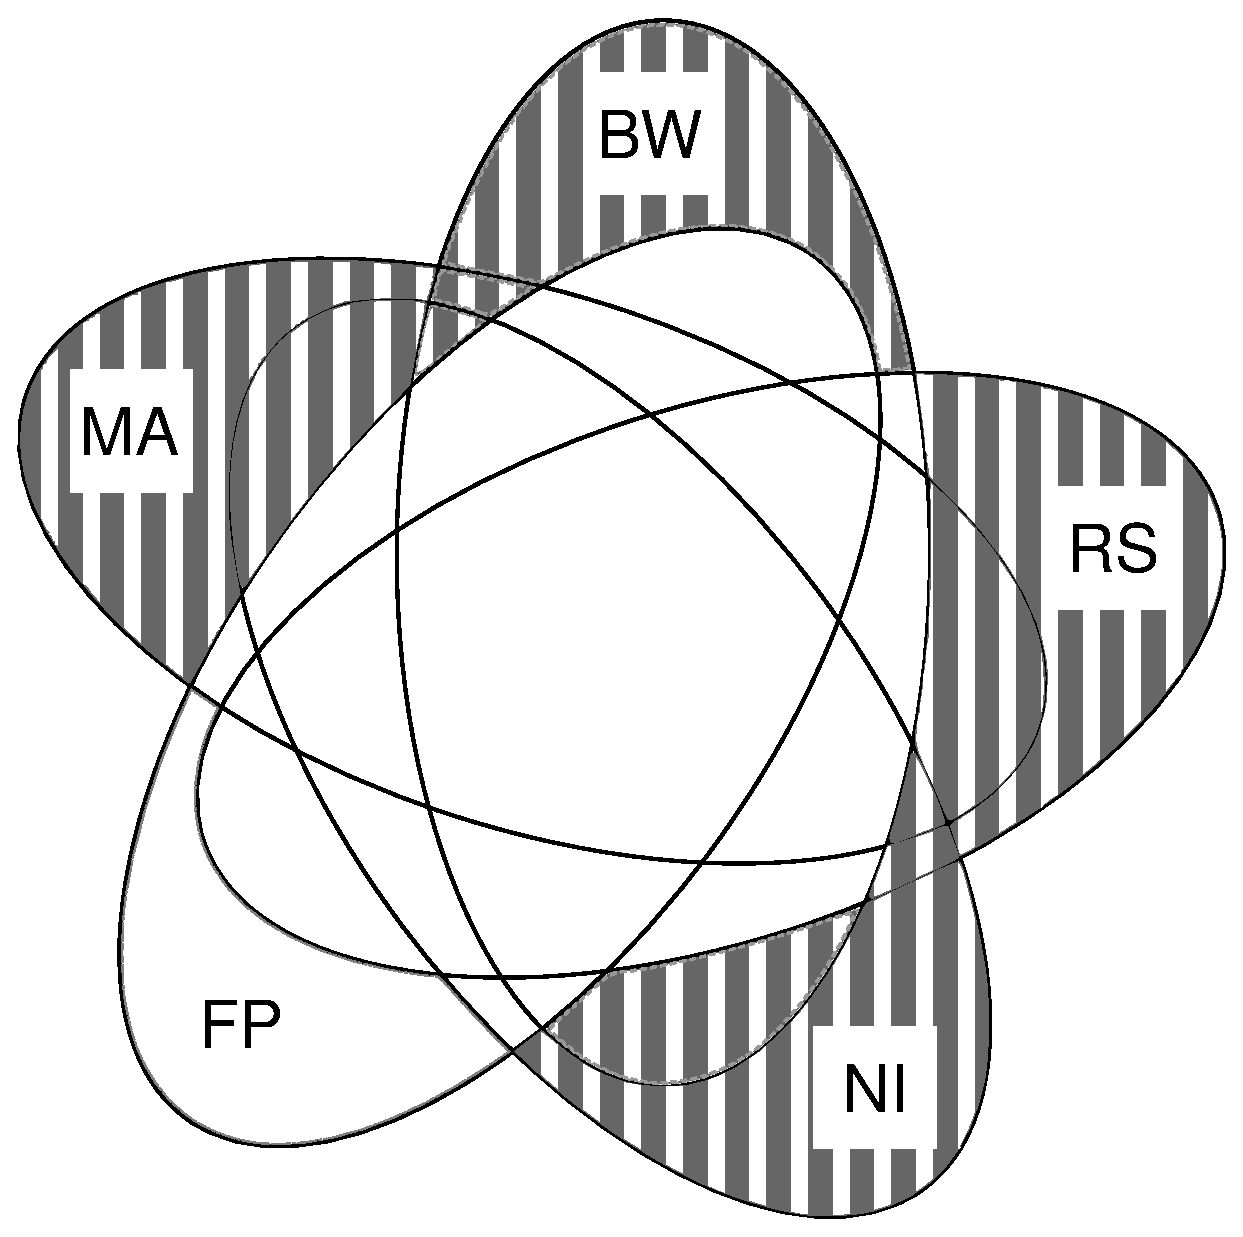
\includegraphics[width=0.49\columnwidth]{figs/static-mapping/venn_matching.pdf}
%\caption{Variants solved by matching approaches.}
%\label{fig:venn_match}
%\end{figure}
This section presents faster algorithms to solve 
two variants of $\CTE$ problem, $\RS+\MA+\NI$ and~$\MA+\NI+\BW$, that can also be solved with the flow approach
introduced above.
First, we consider the~$\RS+\MA+\NI$ variant.
Recall that in this variant,
we are given a~set of redundant chunks ($\RS$) and a~set of nodes
at fixed locations (no $\FP$). The number of~chunks may be larger than the number
of nodes ($\MA$), and each node needs to be connected
to its chunks as well as to other nodes ($\NI$).

\parag{Algorithm.} Due to Observation~\ref{obs:nofp}, the $\RS+\MA+\NI$ variant degenerates to~$\RS+\MA$.
In order to solve the latter,
we construct a bipartite
graph between the set
of nodes and
the set of chunks.
First, we clone each node~$\MaFactor$ times
as each node needs to process
$\MaFactor$ chunks, and we aggregate all replicas of a given chunk in a
single %$\ChunkType$
super-vertex.
Second, we link (cloned) nodes to (aggregated) replicas.
In instances without $\BW$, mapping of any replica to any node is feasible, and hence, for a given mapping $\mu$ of chunks to nodes, the minimum bandwidth is utilized if for each $c$, node $\mu(c)$ serves the closest replica of $c$.
Therefore, for each node $v$ and chunk $c$, we connect each copy of $v$ and the super-vertex $c$ with the link of cost $\min_i \dist(v,c^{(i)})$, i.e., the cost of reaching the closest replica.
Finally, on the resulting bipartite graph, we compute a~\emph{minimum weight
perfect
matching}:
the resulting matching describes the optimal assignment of chunks to nodes.
An example instance is presented in Figure~\ref{fig:matching}.


\begin{figure}
  \centering
  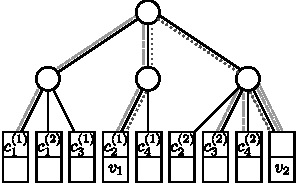
\includegraphics[width = 0.39\columnwidth]{figs/static-mapping/model_ma_r_cv_boxes}
  \centering
  \hspace{1cm}
  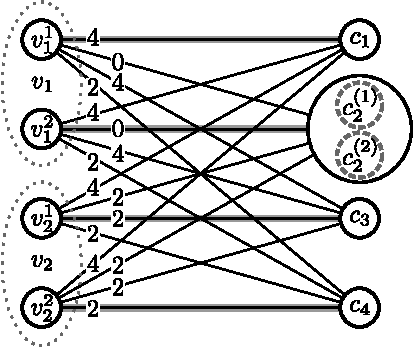
\includegraphics[width =0.39\columnwidth]{figs/static-mapping/matching}
\caption{The~$\RS+\MA$ variant on the left is converted into a
  matching problem instance on the right.
The figure illustrates
an instance where two nodes are
cloned into~$\MaFactor = 2$ nodes each,
resulting in a total of four nodes in
the matching representation.
The two replicas of each chunk are
aggregated into a single chunk vertex~$\achunk_j$  in the matching instance;
this gives a total of four chunk vertices in the matching graph. The costs
on the links between all clones of a specific vertex and a chunk are set to
the minimum distance. For instance, the weights of edges connecting
the two clones of~$\VirtualNode_1$ to~$\achunk_2$ are 0.
}
\label{fig:matching}
\end{figure}

\parag{Analysis.}
The runtime consists of two parts: the construction of the matching graph and
the~actual matching computation. The constructed graph consists of
$\MaFactor \cdot (n_V \cdot \ChunkType) = \tau^2$
many edges,
and for each edge we compute its weight. The shortest distances
in a tree of size $n_S$ can be computed in time~$\mathcal{O}(n_S + q)$~\cite{offline-lca}, where $q$ is the number of queried pairs, which translates to the overall construction time~$\mathcal{O}(n_s + n_v\cdot \sum_{i=1}^\tau r_i)$.
The state-of-the-art algorithm to compute matchings in bipartite graph~\cite{matching-best} has a running time of $\tilde{\mathcal{O}}(|E|^{10/7}\cdot \log W)$, where $|E|$ is the number of edges, $W$ is the maximum weight of an edge, and $\tilde{\mathcal{O}}$ hides polylogarithmic (in terms of $|E|$) factors.
The total running time is then $\tilde{\mathcal{O}}(\tau^{20/7}\cdot \log(n_s)) + \mathcal{O}(n_s + n_v\cdot \sum_{i=1}^\tau r_i)$.
The matching-based algorithm outperforms the flow-based algorithm.


\subsubsection{Local matching algorithm}

Now, we present the way to solve the~$\MA+\NI$ variant even faster by using greedy approach.
Moreover, we show that we can
even solve
$\MA+\NI+\BW$ variants by simply
verifying feasibility.
In~the~following, due to Observation~\ref{obs:nofp}, we can focus on
the~$\MA$ and~$\MA+\BW$ variants, respectively.
We start by lower-bounding the required bandwidth allocation.
The \emph{uplink} of a~proper subtree $T'$, denoted $\Uplink(T')$ is an edge from the root of $T'$ to its parent.

%We first introduce the following definition.
%\begin{defn}[Local Assignment (LA)]\label{def:loc}
%We define an assignment~$\VmChunkAssignment$ to
%be \emph{local in a specific subtree~$\Tree'$}, iff~$\VmChunkAssignment$
%assigns the maximum number of chunks in the
%subtree to nodes in the same subtree.
%We define~$\VmChunkAssignment$ to be \emph{local} when
%it is local with respect to all possible subtrees of the~substrate network.
%\end{defn}
%
%\begin{figure}
%\center
%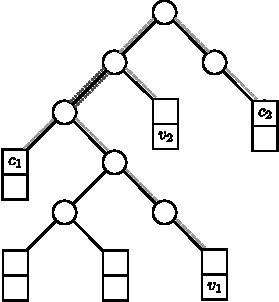
\includegraphics[width = 0.45\columnwidth]{figs/static-mapping/unbalanced_tree}
%\caption{Illustration of local assignment: The dashed lines indicate bandwidth allocations, which occur
%independently of the chosen assignment. The dotted lines indicate bandwidth
%allocation which occur only if~$c_2$ is assigned to~$v_1$.}
%\label{fig:unbalanced_tree}
%\end{figure}
%
%\parag{Example.}
%Figure \ref{fig:unbalanced_tree} illustrates the concept of local assignment:
%The closest chunk to~$v_2$ is~$c_1$, and the closest node to~$c_1$ is~$v_2$.
%However, a subtree~$T'$ exists such that~$v_1 \in T'$ and~$c_1
%\in T'$, but~$v_2 \notin T'$. Therefore, a local assignment cannot assign~$c_1$ to~$v_2$.


%Later we will see that
%optimal solutions to
%$\MA$ have a local assignment. We exploit this in our algorithms described
%in the following.


\begin{lemma}\label{lem:uplink-alloc}
Given the~$\MA$ variant and a proper subtree~$\Tree'$
containing~$\tau(T')$
chunks and~$x$ nodes, the bandwidth allocation of any
assignment
$\VmChunkAssignment$ on the uplink of~$\Tree'$ is at~least $\CostTrans\cdot|\tau(T')-x\cdot\MaFactor|$.
\label{lemma:uplink}
\end{lemma}
\begin{proof}
In case the number of chunks equals the processing capacities of the
nodes in the given subtree,
the bandwidth allocation inflicted by the chunk access network on the uplink is zero, since we can assign all chunks to nodes in the same subtree.
Otherwise, we distinguish between two cases. If there are more chunks in the subtree, at least all excess chunks have to
be mapped to nodes outside $T'$, which 
inflicts costs~$\CostTrans$ per excess chunk on the uplink of~$\Tree'$.
 Similar situation occurs if the processing capabilities exceed the
amount of
available chunks.
Hence, the minimum bandwidth allocation for the chunk access on the uplink
is the absolute difference between the number of chunks and the processing capabilities
of the subtree, i.e.,~$|\tau(T')-x\cdot\MaFactor|$ times $\CostTrans$.
\end{proof}


\parag{Algorithm.} Our proposed algorithm for the $\MA$ variant of $\CTE$
proceeds in a bottom-up fashion, traversing the~substrate network~$\Tree$
from the leaves toward the root.
For each subtree~$\Tree'$, we maintain
two sets~$S_c,S_v$ in order to match unmatched
chunks~$S_c$ in the subtree~$\Tree'$ to unmatched
nodes~$S_v$ in~$\Tree'$. Both sets are initially empty.
We associate a counter with each node that enters $S_v$, and we intitialize it to $\MaFactor$, the multi-assignment factor.


We first process all the leaves, in an arbitrary order; subsequently, we process inner vertices
of~$\Tree$ whenever all their children have been processed.
We process any leaf~$\ell$
by adding any
nodes or chunks which are located on~$\ell$ to the corresponding sets~$S_c$ and~$S_v$.
A non-leaf vertex~$u$ is processed in the following way: we take the union of
the sets corresponding to~$u$'s children, i.e., the sets contain the unmatched chunks and nodes
in this subtree.
For both leaves and inner nodes, whenever
both sets are non-empty, we greedily match an arbitrary chunk $c$ in~$S_c$ with an arbitrary node $v$ in~$S_v$.
Then, we remove $c$ from $S_c$, and we decrement the counter of $v$. If the counter of $v$ reaches zero, we remove $v$ from $S_v$.

\parag{Analysis.} For each
vertex in the substrate graph,
we build the union of the
children's sets.
The number of all remove operations is equal to
the number of chunks~$\mathcal{O}(\ChunkType)$.
Hence the overall complexity of this construction amounts to
$\mathcal{O}(n_S + \ChunkType)$.
The local matching algorithm outperforms the previous algorithm that relied upon calculating the minimum-weight perfect matching.

%It remains to prove optimality of such local assignments.
%By \emph{uplink} of a subtree with root $r$ we denote the edge from $parent(r)$ to $r$ (if it exists).
%We first characterize the bandwidth allocation on uplinks of subtrees.

%\begin{theorem}
%Given an~$\MA+\NI$ variant instance, a feasible assignment~$\VmChunkAssignment$
%is optimal iff it is local.
%\label{thm:local_optimal}
%\end{theorem}
%
%\begin{proof}
%Local assignments generate exactly the minimal allocations on all links, as
% the assignments which generate the minimal bandwidth allocations
%described in
%the proof of
%Lemma~\ref{lemma:uplink} are local in the given subtree. Hence
%each local assignment has to be optimal. A non-local assignment, has at least
%one subtree, in which it is not local. This subtree has a higher
%allocation on the uplink. Since the local assignment has minimal allocations
%on all other links, the non local assignment has a larger footprint.
%\end{proof}

The algorithm allocates the minimum possible bandwidth at an uplink of every subtree, as stated in Lemma~\ref{lemma:uplink}, and hence the algorithm computes an optimal solution.
Combined with a~simple postprocessing step, this approach can also solve~$\MA+\BW$ variant. The central idea of this extension is
that the algorithm allocates the minimal bandwidth
on each individual edge. In consequence, any bandwidth constraint,
which is lower than the allocation of a local assignment on one link, renders
the problem infeasible. Hence, it is sufficient to temporarily omit the
bandwidth limitations, compute an optimal assignment for an~$\MA$ instance, and
verify that the resulting allocations do not violate any capacities. The
postprocessing step scales linearly with the number of edges in the substrate
graph.


\subsection{Dynamic Programming}\label{ssec:dyn}

We now show how to solve the~$\MA+\FP+\NI+\BW$ variant
in polynomial time.
Note that this variant requires to find a
tradeoff between the desire to place nodes as close as possible to each other
(in order to minimize communication costs), and the desire to place nodes
as close as possible to
the chunk locations.




\parag{Example.} Figure~\ref{fig:dynamic_motivation} shows an example: one
extreme solution is to minimize the distance between chunks and nodes,
see mapping~$\NodeMapping_1$ in the left picture in
Figure~\ref{fig:dynamic_motivation}: the four nodes are all
collocated with chunks, resulting in a zero-cost chunk access network. As a
result, the paths between the individual nodes are longer than in alternative
node placements: each node has a~distance of two hops to one other node,
and four hops to two other nodes. Hence the resulting allocations for the
node inter-connect sum up to~$20 \cdot \CostCom$.

%\begin{figure}[t]
%\centering
%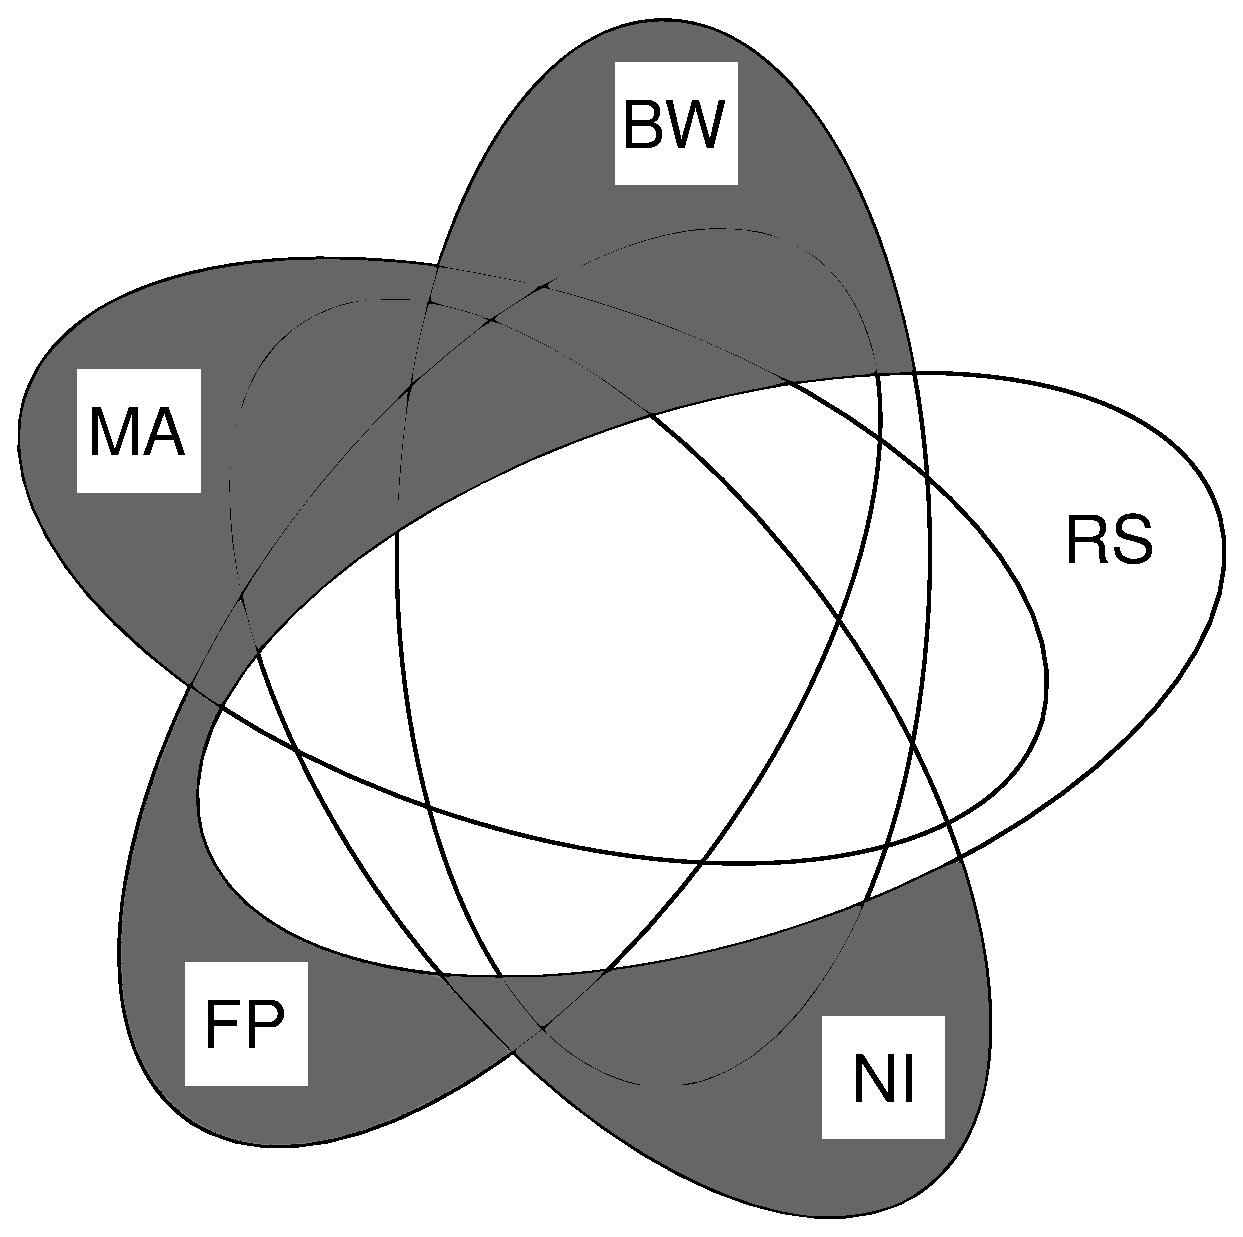
\includegraphics[width=0.49\columnwidth]{figs/static-mapping/venn_dp.pdf}
%\caption{Variants solved by dynamic programming approach.}
%\vspace{-1em}
%\label{fig:venn_dp}
%\end{figure}

The right picture in Figure~\ref{fig:dynamic_motivation} shows a different node
mapping~$\NodeMapping_2$, which seeks to minimize the inter-connect costs
between the nodes, and places all nodes in one subtree. The distance between all
nodes is two, which results in a total bandwidth allocation of~$12\cdot\CostCom$
for the inter-connect. However, this reduced price comes at additional costs in
the access network:~$c_3$ and~$c_4$ have to be mapped to~$v_3$ and~$v_4$,
which requires a total bandwidth allocation of~$8 \cdot \CostTrans$.


\begin{figure}
  \centering
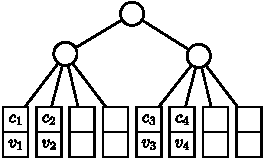
\includegraphics[width = 0.39\columnwidth]{figs/static-mapping/dynamic_bad}
\hspace{1cm}
\centering
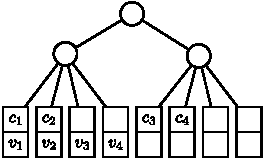
\includegraphics[width = 0.39\columnwidth]{figs/static-mapping/dynamic_good}
\caption{Two different node placements for the same substrate graph and chunk
locations. For~$\CostTrans = \CostCom$, both solutions have an identical
footprint. In other cases, one solution outperforms the other.}
\label{fig:dynamic_motivation}
\vspace{-1em}
\end{figure}



\parag{Algorithm.} Our proposed approach is based on dynamic programming, and
leverages the \emph{optimal substructure property} of the $\MA+\FP+\NI+\BW$ variant:
as we will see, optimal solutions for subtrees
can be efficiently combined into optimal solutions for the whole tree.
First, we transform the
substrate network~$\Tree$
into a binary tree:
we clone every higher-degree node,
iteratively attaching additional clones as right children
and original children as left descendants.
New edges between cloned vertices constructed during the binarization have infinite capacity.

As usual in dynamic programs, we define, over the structure of the tree, a
recursive formula~$f$ for
the minimal cost solution given any possible number of nodes
embedded in a given subtree (the actual set of nodes does not matter,
due to symmetry).
The value of $f(T', x)$ corresponds to the minimum bandwidth cost of placing $x$ nodes in a subtree $T'$.
It is defined as the bandwidth allocated inside $T$ plus the bandwidth allocated on the uplink of $T'$.
The latter is equal to
\[
bw(T',x) = 
    \CostTrans\cdot|\tau(T')-x\cdot\MaFactor| +\CostCom \cdot
(\Vms - x) \cdot x\enspace, \\
  \]
  where $\tau(T')$ is the number of chunks in a~subtree~$T'$.
  If~$bw(T',x)$ exceeds the capacity~$\capacity$ of the uplink of $T'$, we set $\b(T', x) = \infty$.
  The first term represents
the bandwidth necessary to transport the chunks in $T'$ from their location to
nodes outside of $T'$ (see Lemma~\ref{lemma:uplink} for similar argument).
The second term of $bw$ represents the required bandwidth for the communication between the~$x$
nodes inside~$T'$, and the~$\Vms - x$ nodes in the remaining parts of the substrate
network.
Then, the formula to calculate the function $f$ for a subtree containing only a leaf $\{ \ell \}$ is
\[
f(\{ \ell \}, x) =
\begin{cases}
   \infty & \mbox{if } x > \capacity(\ell)\enspace,\\
    bw(\{ \ell \}, x) & \mbox{otherwise}\enspace. \\
  \end{cases}
  \]
We set~$f(\{ \ell \},x)$ to infinity if $x$ exceeds the node hosting capacity of server $\ell$.

To calculate the value of $f(T', x)$ for non-leaf subtree $T'$, we split the~$x$ nodes
into two positive integer
values $r$ and $x-r$, and we put~$r$ on the right and~$x - r$ on the left subtree.
That is, we take the optimal cost
(given recursively) of placing~$r$ nodes in
the right subtree~$\textsc{Ri}(T')$ of~$T'$ and~$x-r$ nodes in the left subtree~$\textsc{Le}(T')$ of
$T'$. Given the cheapest combination, we add the bandwidth requirements
on the uplink of~$T'$ to generate the overall costs for placing~$x$ nodes in~$T'$, obtaining
\[
  f(T', x) = 
    \min_{0\leq r \leq x} \{  f\left(\textsc{Le}(T'),
x-r\right) +
f\left(\textsc{Ri}(T'), r\right) \} + bw(T',x)\enspace.
  \]

We compute~$f$ in a bottom-up manner. 
To finally compute the actual optimal embedding,
we traverse the computed minimal-cost path backwards,
according to
the optimal values found for~$f$ during the bottom-up computation.


\parag{Analysis.}
The substructure optimality follows from the observation that
costs can be accounted on the uplink, and the fact
 that we check each possible node distribution.
For each substrate vertex ($n_S$ many) we have
to check the cost of all possible splits,
resulting in an overall complexity of~$\mathcal{O}(n_S \cdot n_V^2)$.
The runtime to binarize~$\Tree$ is asymptotically negligible in comparison.


\subsection{Simple Variants}

%\begin{figure}
%\centering
%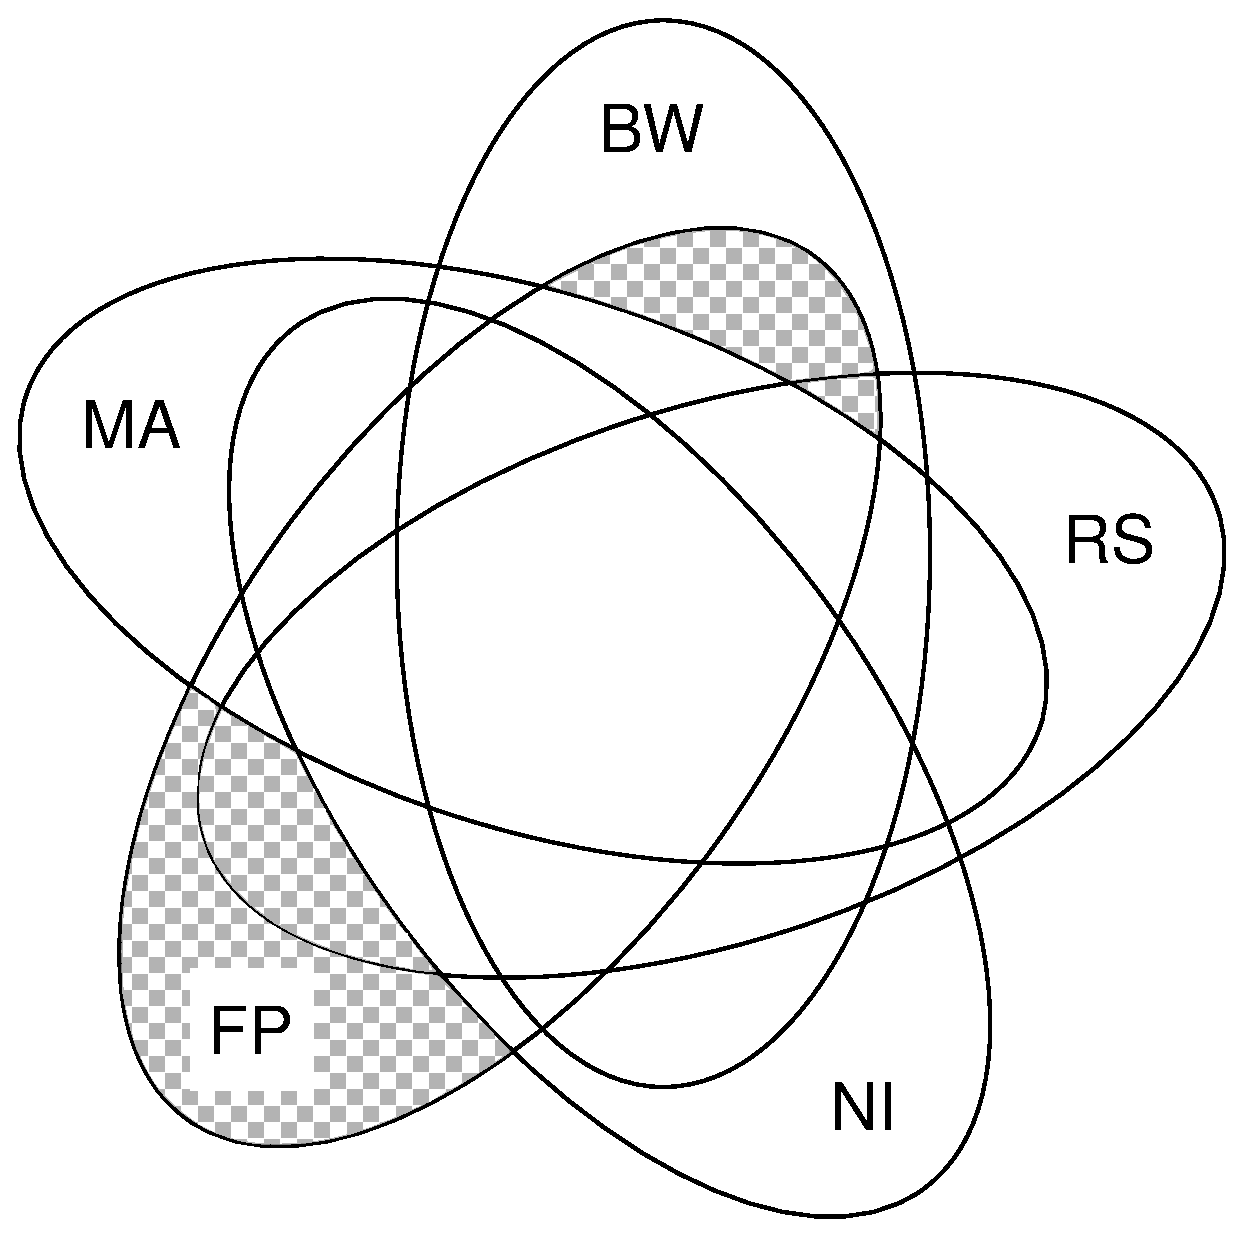
\includegraphics[width=0.49\textwidth]{figs/static-mapping/venn_trivial.pdf}
%\caption{Trivially solvable variants.}
%\label{fig:venn_trivial}
%\end{figure}


For the sake of completeness, we also observe that there are
several variants that admit a trivial solution. Concretely, variants with~$\FP$
plus any combination of
$\RS$ and~$\BW$ (but without~$\MA$ and~$\NI$) can easily be solved by
mapping
nodes to chunk locations.
%Figure~\ref{fig:venn_trivial}
%shows a Venn diagram of the trivial property combinations.

%%%%%%%%%%%%%%%%%%%%%%%%%%%%%%%%%%%%%
\section{NP-Hardness Results}\label{sec:np}

We have seen that even variants with multiple dimensions of
flexibility can be solved optimally in polynomial time.
This section now points out fundamental
limitations in terms of computational tractability.
In particular, we
show that variants become NP-hard if flexibly placeable nodes ($\FP$) have to be assigned to one of multiple replicas ($\RS$), either with multiple chunks per node ($\MA$ in Section~\ref{ssec:fprsma}) or with communication among nodes ($\NI$ in Section~\ref{ssec:fprscc}).
Both results hold even in uncapacitated networks, and even in small-diameter
substrate networks (namely two- or three-level trees).
Clearly, the hardness of variants $\FP+\RS+\MA$ and~$\FP+\RS+\NI$ imply
the hardness of more general variants.

In addition to hardness results for the aforementioned $\CTE$ variants, we study the influence of restricting number of replicas of a chunk on computational tractability on these variants.
Namely, we introduce the restricted replica selection component $\RS(r_{max})$, parametrized by an~integer $r_{max}$, that restricts the number of replicas of any chunk: for every chunk $c_i$ we have $r_i \leq r_{max}$.
We consider $\RS(2)$ component in relation with Multi-Assignment ($\MA$).
Concretely, in Section~\ref{ssec:fprsma}, we first present the NP-hardness of the unrestricted scenario $\FP+\RS+\MA$ (Theorem~\ref{th:ma-unlimited}) as a warm-up,
and then we present more refined hardness result for $\FP+\RS(2)+\MA$ (Theorem~\ref{th:ma-reduction}).
In Section~\ref{ssec:fprscc}, we present the NP-hardness of the unrestricted scenario $\FP+\RS+\NI$ (Theorem~\ref{theorem:fp_rs_cc}).
%However, restricted replica selection $\RS(2)$ in combination with Node-Interconnect requires additional ways to control the placement of nodes, and the NP-hardness result uses bandwidth constraints $\BW$~\cite{my-tcs}.

\subsection{Introduction to 3D Perfect Matching}
\label{sec:3dm_intro}

The hardness of both~$\FP+\RS+\MA$ and~$\FP+\RS+\NI$ variants of the $\CTE$ problem uses a reduction
from the NP-complete problem of \emph{3D Perfect Matching}~\cite{3dmatch},
which can be seen as a generalization of bipartite matchings to 3-uniform
hypergraphs. We refer to this problem by~$\TDM$
review it quickly for completeness.
$\TDM$ is defined as follows: we are given three finite and disjoint
sets~$X$,~$Y$, and~$Z$ of cardinality~$k$, as well as a~subset of triples~$P\subseteq
X \times Y \times Z$.  Set~$M \subseteq P$ is a 3-dimensional matching
if and only if, for any two distinct triples~$t_1=\langle x_1, y_1, z_1\rangle \in M$
and~$t_2= \langle x_2, y_2, z_2 \rangle \in M$, it holds that~$x_1\neq x_2$,~$y_1\neq
y_2$, and~$z_1\neq z_2$. The goal is to decide if we can construct
a subset of triples $M \subseteq P$ that is \emph{perfect}, i.e., covers all
elements of~$X \cup Y \cup Z$ exactly once.


\subsection{Hardness of Multi-Assignments}\label{ssec:fprsma}

%\subsubsection{Warm-up: Multi-Assignment with Unrestricted Number of Replicas}
The proof of hardness of the $\FP+\RS+\MA$ variant of the $\CTE$ problem is based on the following construction.
Let~$\ITDPM$ be an instance of~$\TDM$ with $p$ triples and set cardinality~$k = |X| = |Y| = |Z|$.
We construct an instance~$\ICTE$ of the $\CTE$ problem in the following way:
\begin{enumerate}
\item \emph{Substrate network:} We construct a substrate network in form of a tree consisting of a root,
and for each triple from $P$, we construct a \emph{triple gadget} which we directly attach as
a child of the root. The gadget is of height 2,
and consists of an inner node and three leaves.
\item \emph{Chunks:} For each element in~$X$,~$Y$ and~$Z$,
 we construct a chunk
($3 \cdot k$ chunks in total). Every gadget contains three chunk replicas (one per leaf),
corresponding to the elements of the triple.
\item \emph{Other properties of the instance:} We set the number of to-be-embedded nodes $n_V = k$,
$\CostTrans = 1$, and the the multi-assignment factor
$\MaFactor=3$.
\item \emph{Threshold.} In order to turn the optimization problem into a decision problem, we use
a~cost threshold~$\Thr = 4\cdot k$. As we will show, the cost threshold is met by all
assignments that assign all three chunks of each triple gadget to a
node which is collocated with one of these chunks, and only by such assignments.
\end{enumerate}

%\parag{Example.} Figure~\ref{fig:fprsma} shows an example of our construction: In an~instance~$\ITDPM$
%of 3-DM sets $X, Y, Z$ consist of the following elements: $X = \{ x_1, x_2 \}, Y = \{ y_1, y_2 \}$ and $Z = \{ z_1, z_2 \}$.
%Set of triples $P$ contains three triples
%$(x_1, y_1,
%z_1)$,~$(x_2, y_1, z_2)$, and~$(x_2, y_2, z_2)$. This instance has only one solution:~$M =
%\{(x_1,y_1,z_1),(x_2,y_2,z_2))\}$.
%
%To construct the corresponding instance~$\ICTE$ of the $\CTE$ problem, we
%create a gadget for each triple in~$P$. For each variable which occurs in a
%triple, the corresponding gadget contains a~chunk of the
%type of the variable. The triple
%$(x_2, y_1, z_2)$ of the instance is represented by the middle gadget in
%Figure~\ref{fig:fprsma}. The objective of~$\ICTE$ is to allocate~$k=2$ nodes
%with the smallest possible footprint. If the total footprint is at most $4\cdot k$, we can construct a solution to~$\ITDPM$ from the solution to~$\ICTE$.
%The footprint consists of the costs which occur when a node is embedded in a~gadget, and the three chunks of that gadget which are assigned to that node: one of
%the chunks is collocated with the node, the other two have to be transferred
%via two hops, incurring unit costs on each hop.


\begin{figure}[t]
  \centering
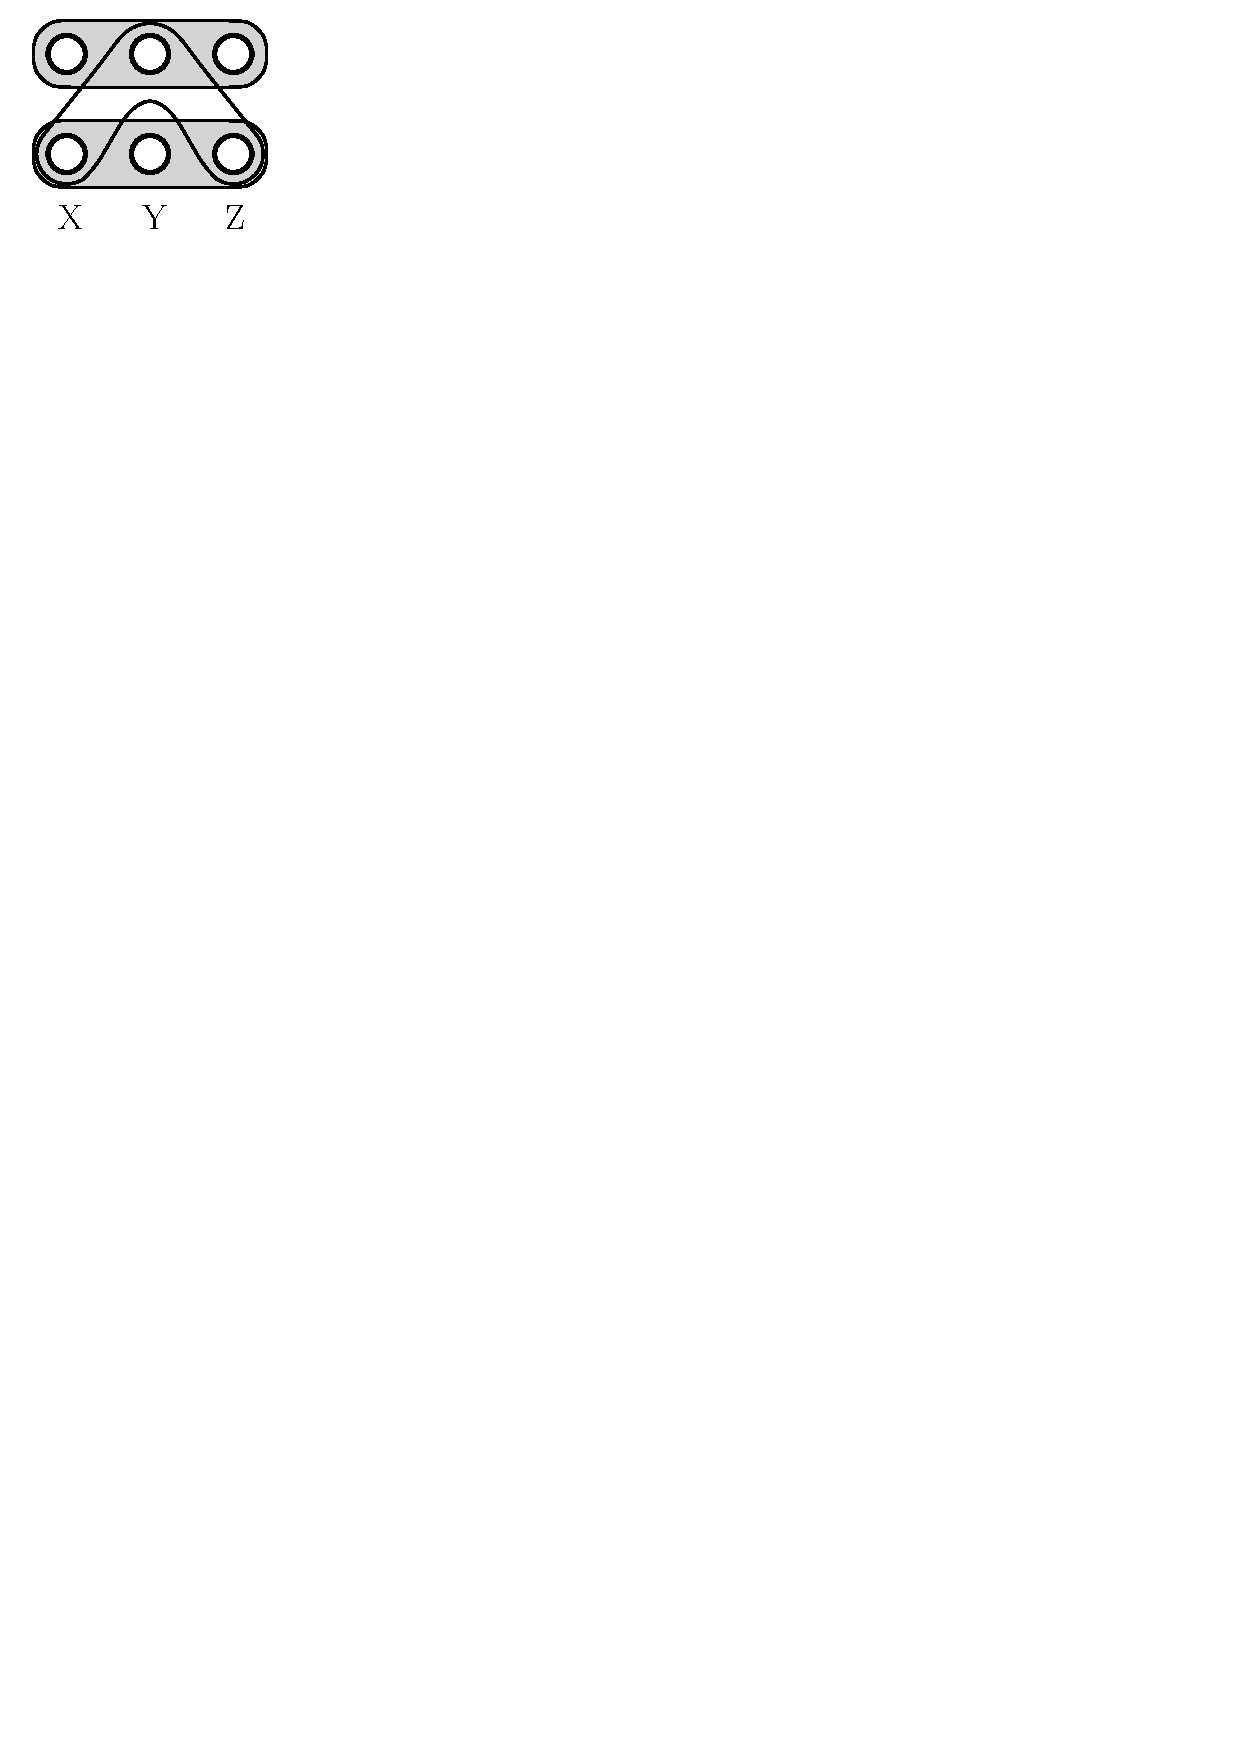
\includegraphics[width = 0.21\columnwidth]{figs/static-mapping/tdm-horizontal}
\hspace{1cm}
\centering
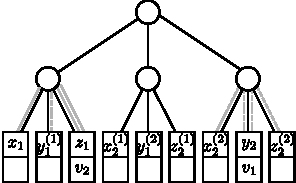
\includegraphics[width = 0.4\columnwidth]{figs/static-mapping/np_3dm_construction}
\hfill
\caption{\textit{Left:} A~$\TDM$ instance of cardinality $k=2$ with three triples:
$\langle x_1, y_1, z_1 \rangle$,~$\langle x_2, y_1, z_2 \rangle$, and~$\langle x_2, y_2, z_2\rangle$. The solution is
indicated by the grey triples. \textit{Right:} The corresponding instance and an optimal solution for the~$\FP + \MA
+ \RS$ of the $\CTE$ problem. Each triple corresponds to a single triple gadget.}
\hfill
\label{fig:fprsma}
\end{figure}

Figure~\ref{fig:fprsma} shows an example of our construction.
Given these concepts, we can now show the computational hardness of the considered variant of $\CTE$ (Theorem~\ref{th:ma-unlimited}).
\begin{theorem}
  The $\FP+\RS+\MA$ variant of the $\CTE$ problem is NP-hard.
  \label{th:ma-unlimited}
\end{theorem}
\begin{proof}
Fix an instance $\ITDPM$ of~$\TDM$ and construct the~$\ICTE$ instance of
the~$\FP+\RS+\MA$ variant in the way described above. We prove that~$\ICTE$ has a solution of cost at most $\Thr = 4 \cdot k$ if ($\Rightarrow$) and only if
($\Leftarrow$)
$\ITDPM$ has a~perfect matching (of size~$k$).

\medskip

($\Rightarrow$) Fix a solution $\STDPM$ for~$\ITDPM$, i.e., the set of triples that form a perfect matching. To construct the solution $\SVCEMB$ to $\IVCEMB$, we place a single node in every
gadget that corresponds to triples in $\STDPM$ (at an arbitrary leaf of this gadget). In each gadget, we match all three chunks to the node located in this gadget. This
solution costs exactly~$\Thr = 4\cdot k$: each of $k$ nodes processes one chunk collocated with it and two chunks at the distance $2$.
The solution $\STDPM$ matches every element of the universe $X \cup Y \cup Z$, hence every chunk is processed by exactly one node, and $\SVCEMB$ is feasible.

\medskip

($\Leftarrow$) Fix a solution $\SVCEMB$ for ~$\ICTE$ with cost at most $\Thr$.
We call the triple gadget \emph{active} if it hosts a single node in one of its leaves.
We claim that $\SVCEMB$ places at most one node in each triple gadget.
Assume that two nodes $x_1$, $x_2$ are placed in the same triple gadget.
First, we lower-bound the cost incurred by $x_1$ and $x_2$ that collectively process $2\cdot \MaFactor = 6$ chunks.
At most two of these chunks are co-located with $x_1$ or $x_2$ and cost $0$, and remaining four chunks incur a cost at least $2$ each.
Moreover, at least three of these chunks are placed outside of this triple gadget and incur the cost at least $4$ each.
In total, $x_1$ and $x_2$ incur the cost at least $2\cdot 0+2+3\cdot 4=14$.
Second, we lower-bound the cost incurred by remaining $k-2$ nodes.
Each node can process at most $1$ of its $\MaFactor=3$ chunks for free (every leaf hosts exactly one chunk),
and it incurs the cost at least $4$ for the remaining~$2$ chunks that are at distance at least~$2$.
The total chunk mapping cost $4\cdot k + 6$ exceeds the threshold $\Thr = 4\cdot k$, a contradiction.
As $n_V = k$, we conclude that in $\SVCEMB$, exactly $k$ active gadgets.

To construct the solution $\STDPM$ to $\ITDPM$, we pick the set of triples whose gadgets are active.
The solution $\STDPM$ consists of $k$ triples.
Since all chunks are processed by exactly one node, every element of~$X$,~$Y$ and~$Z$ is matched, and $\STDPM$ form a 3-dimensional perfect matching of $X \cup Y\cup Z$.
\end{proof}

\subsection{Hardness of Multi-Assignments with at Most Two Replicas}

%We have seen that replica selection flexibility can render embeddings computationally hard.
We provide a more detailed look at this hardness result
and explore the minimal requirements for rendering replica selection hard.
Concretely, we show that already two replicas for each chunk are sufficient for computational intractability.

% We now show that the 2-replica selection variant is even NP-hard
%without capacity constraints.  In particular, we consider the 
%variant~$\RS(2)+\MA(4)+\FP$ with at most two replicas of each chunk and assignment factor
%four. There are no capacity constraints on links.
%
%Our construction consists of two major modifications to hardness result without replication factor restrictions (for that result, refer to Section~\ref{ssec:fprsma}).
%
%\parag{Unique chunks on the comb.} First, we provide the tools for restricting the placement of nodes in certain parts of the tree.
%In Section~\ref{ssec:fprsma}, due to symmetric structure of the tree, the carefully crafted threshold value allowed us to prove that e.g. no Triple Gadget ever had two or more nodes placed in it.
%We still use the threshold value as the placement mechanism, but in this section, due to the asymmetrical tree construction, we combine it with the concept of unique chunks on the comb (by \emph{comb} we denote the balanced tree, where all non-root vertices have at most one child).
%
%For an introduction to the concept of unique chunks, let us consider the following example.
%Suppose that within one $\VCEMB$ construction, we would like to encode not one $\TDPM$ instance, but two $\TDPM$ instances: $M_1$ and $M_2$, with disjoint universe and different number of triples to be chosen: $n_1$ and $n_2$.
%We perform the following modifications to the encoding provided in Section~\ref{ssec:fprsma}.
%The multi-assignment factor grows by $1$, that is the instance we construct is the $\RS+\MA(4)+\FP$ variant instance.
%We construct two subtrees $T_1$ and $T_2$, that correspond to $M_1$, resp. $M_2$; we construct two two-edge-level combs $C_1$ and $C_2$, with number of leaves $n_1$, resp. $n_2$.
%We attach $M_1$ and $C_1$ (resp. $M_2$ and $C_2$) to the common root and we name the resulting subtree $P_1$, resp. $P_2$.
%Next, we attach $P_1$ and $P_2$ to the common root.
%In the end, the height of the tree grew by $2$.
%Finally, we populate both combs with unique chunks, and we set the number of to-be-placed nodes to $\Vms = n_1+n_2$.
%We modify the threshold to be the sum of the thresholds for constructions for $M_1$ and $M_2$ plus $4\cdot (n_1 + n_2)$.
%The last substrate of the threshold value corresponds to transportation of the fourth chunk processed by each machine for the distance of four.
%
%To see why the example indeed can solve two instances of $\TDPM$, we need the following observations.
%First, we claim that no node is ever placed in a comb.
%To prove this fact, we use the property of the comb that the leaves are highly separated, and the fact that each machine has to process $4$ chunks.
%Next, we claim that the number of nodes placed in $P_1$ (resp. $P_2$) is $n_1$ (resp. $n_2$).
%To see this, consider any imbalance of the number of placed nodes; notice that some chunks in the underpopulated comb are processed outside of their $P_i$ subtree, resulting in the solution that exceeds the threshold.
%
%\parag{Families of chunks.} The second tool that we introduce allows us to express the redundancy of chunks without actually replicating chunks more than two-fold.
%For simplicity of introduction, we consider the scenario with no multi-assignment.
%For each chunk $c$ with redundancy, we count the number of occurrences of replicas of such a chunk in the tree, and name it $r_c$.
%We replace the chunk $c$ with $r$ chunks, which we call the family $F_c$ of that chunk.
%For each occurrence of replica of $c$, we replace it with a replica of any chunk from the family (without repetitions).
%To this point, the redundancy factor was reduced from $r_c$ to $1$.
%Now, we construct the gadget $G_c$ for chunk $c$, which consists of $r_c$ leaves, each hosting the second replica of each chunk from family $F_c$.
%We use the technique of unique chunks on the comb to constraint the number of nodes in $G_c$ to be exactly $r_c - 1$.
%We provide necessary additional $r_c-1$ nodes to be placed.
%Hence, exactly $1$ node is placed on a chunk of family $F_c$ outside the gadget $G_c$, and exactly $r_c-1$ nodes cover the remaining $r_c-1$ chunks inside gadget $G_c$.
%All chunks are processed, the replication factor is reduced to $2$, and the size of construction grows polynomially.

%\parag{Introduction to the reduction.} As we already stated, we modify the construction from Section~\ref{ssec:fprsma}.
%As a way to deal with replication, we use the families of chunks using the unique chunks on the comb.
%We extend the construction of a gadget for chunk with redundancy, by incorporating the fact that the multi-assignment factor is $4$.
%For the construction to remain correct given such a multi-assignment factor, we introduce further chunks with one chunk replica to place in the chunk gadget and use the excessive $3$ data processing capacities.

For an arbitrary instance~$\ITDPM$ of the~$\TDM$ problem we construct a~$\RS(2)+\MA+\FP$ variant instance~$\IVCEMB$ the following way.
Let $k = |X|=|Y|=|Z|$ and $p = |P|$.
For each element $e\in X\cup Y\cup Z$, by $P_e$ we denote the set of all triples that contain $e$.
Let $\deg(e) = |P_e|$, and note that $\sum_e \deg(e) = 3\cdot p$.
We proceed with the construction as follows.
\paragraph{Substrate network.}
We construct the substrate network that consists of two subtrees connected to the
  root: a \emph{\MatchSubtree} and a \emph{\CoverSubtree}. The
  {\MatchSubtree} consists of $p$ \emph{\TripleGadgets} (one per each triple from $P$) and $k$
  \emph{\UnqGadgets}. The {\CoverSubtree} consists of~$3\cdot k$ \emph{\ElGadgets} $G(e)$, one for each element $e\in X\cup Y\cup Z$.
  The contruction is depicted in Figure~\ref{fig:red-ma2}.
\begin{figure}[t]
  \centering
  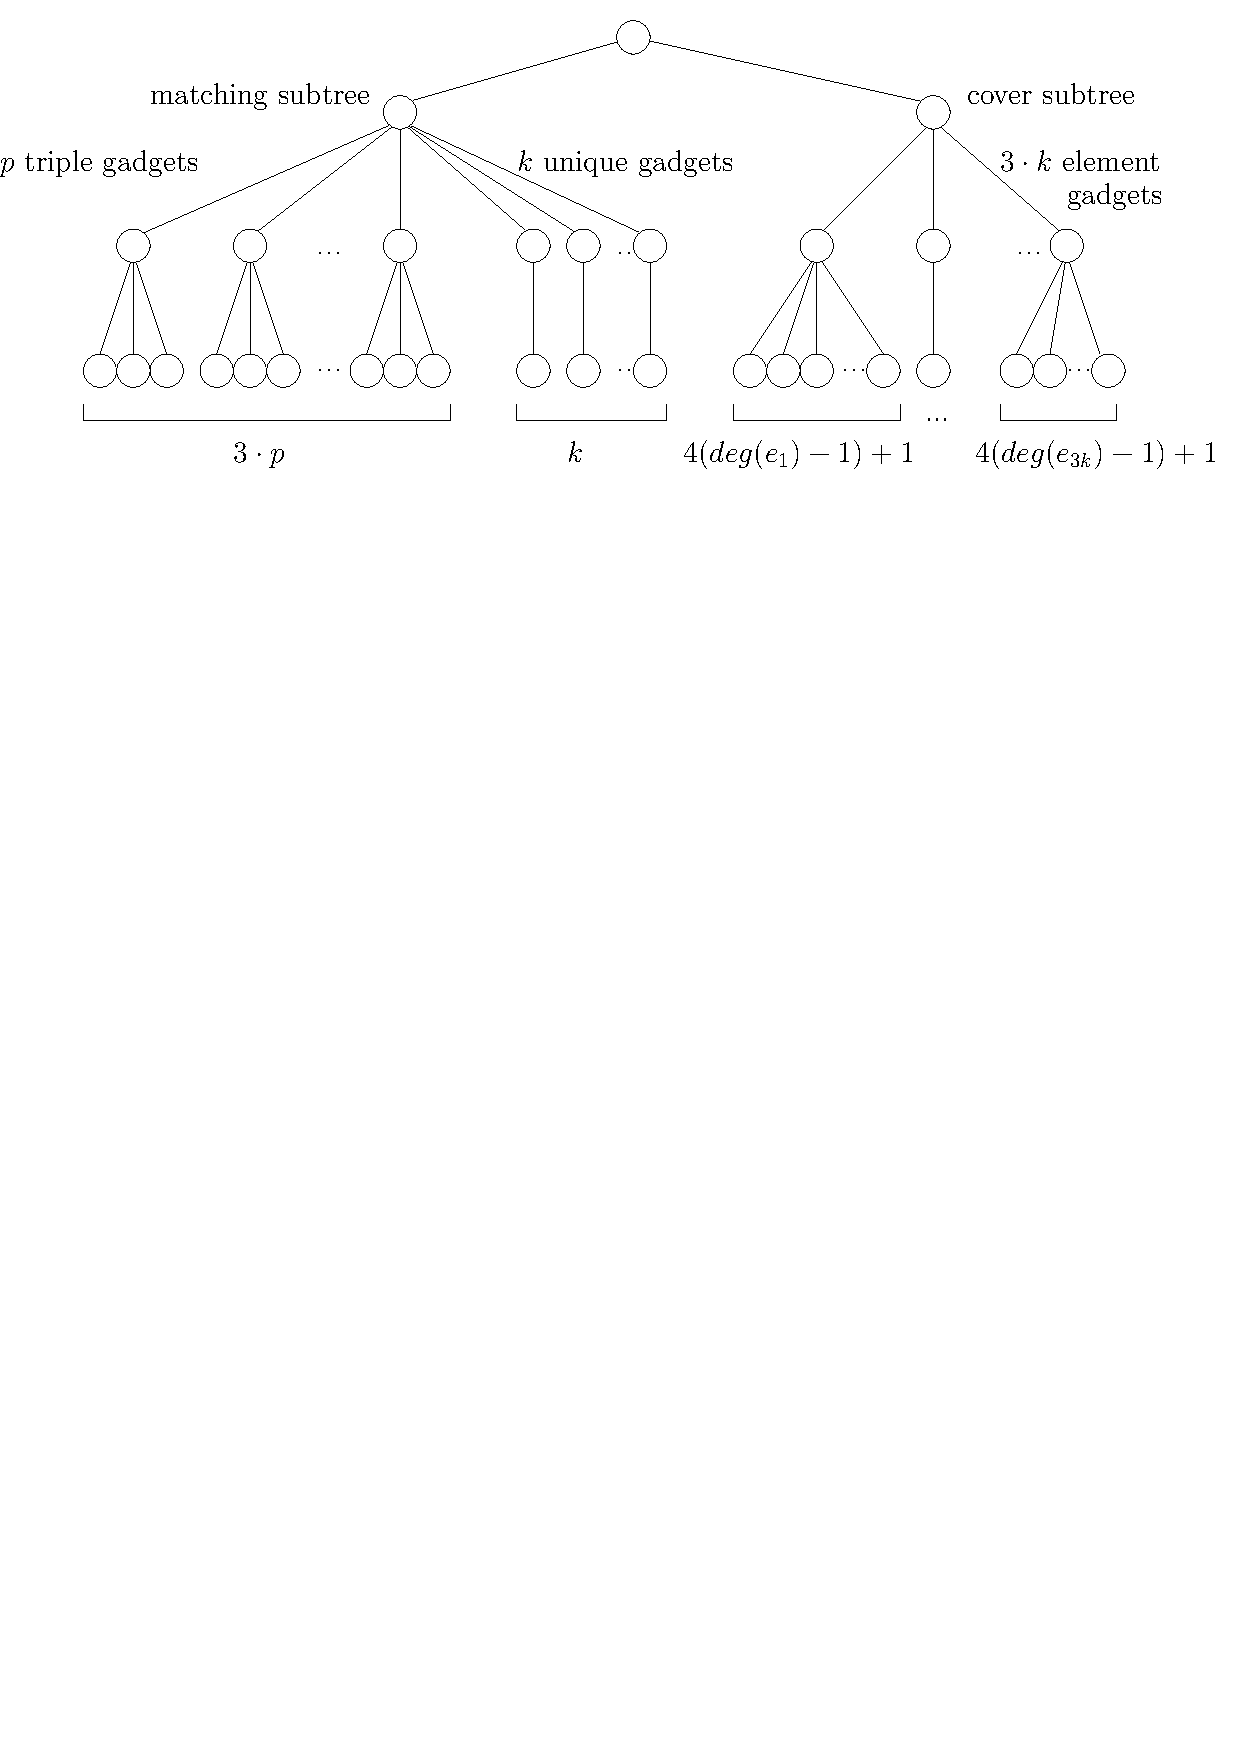
\includegraphics[width=0.9\columnwidth]{figs/static-mapping/overview}
  \caption{Overview of the substrate network in the proof of the NP-hardness of $\FP+\RS(2)+\MA$ variant of $\CTE$.}
  \label{fig:red-ma2}
\end{figure}

\noindent Gadgets are constructed in the following way:
\begin{enumerate}
  \item Each {\TripleGadget} consists of four vertices: three leaves and the root of the gadget, as defined in the reduction for the $\FP+\RS+\MA$ variant in Section~\ref{ssec:fprsma}.
  \item Each {\UnqGadget} consists of two vertices: the leaf and the root of the gadget.
  This keeps the tree balanced, and also keeps leaves of
  {\UnqGadgets} far from each other.
  \item The {\ElGadget} $G(e)$ for element $e$ consists of the
  root and~$4\cdot(\deg(e)-1)+1$ leaves. There are $3\cdot k$ elements numbered from $e_1$ to $e_{3\cdot k}$, and $3\cdot k $ corresponding element gadgets.
\end{enumerate}

\paragraph{Chunks.}
We construct three sets of chunks.
The first set corresponds to elements of the universe $X\cup Y\cup Z$, and their construction is similar to construction of chunks in Section~\ref{ssec:fprsma}, but it takes the restricted replication factor into consideration.
%Namely, for each element of universe $e \in X \cup Y \cup Z$, we construct $\deg(e)$ chunks, each having two replicas.
%The set of $k$ \emph{unique} chunks is placed in the unique subtree and their role is to enforce the placement of exactly $k$ nodes in the matching subtree.
%We place $3\cdot(\deg(e) - 1)$ \emph{dummy} chunks in the element gadgets; each node in the element subtree needs to processes only $1$ element chunk and remaining $3$ of $\MaFactor=4$ chunks are the dummy chunks.
%Unique and dummy chunks have one replica, and we simply identify the chunk with chunk replica.
\begin{enumerate}
  \item \emph{Element chunks}. For each triple $t = \langle x, y, z \rangle \in P$, we construct $3$ chunks:~$c(x, t), c(y, t),$ $c(z, t)$, i.e., $\sum_e\deg(e)$ $=3\cdot p$ chunks in total,
  each having two replicas.
  First replicas are placed in the matching subtree:
  we place
  three replicas: $c^{(1)}(x, t), c^{(1)}(y, t)$ and $c^{(1)}(z, t)$ in the {\TripleGadget} for triple $t\in P$, one per each leaf.
  Second replicas are placed in the cover subtree:
  for each element $e \in X\cup Y\cup Z$, for each $t \in P_e$,
  we place replicas $c^{(2)}(e, t)$ in the leaves of the gadget $G(e)$.
  \item \emph{Unique chunks}. We construct~$k$ unique chunks with one replica each, and we place these replicas at the leaves of {\UnqGadgets} (one chunk per leaf).
  \item \emph{Dummy chunks}. For each element~$e\in X\cup Y\cup Z$,
  we construct an additional set of $3\cdot(\deg(e) - 1)$ dummy chunks, with one replica each, and we place these replicas in arbitrary $3\cdot (\deg(e)-1)$ leaves of $G(e)$ (one chunk per leaf).
  Recall that the remaining $\deg(e)$ leaves of $G(e)$ contain replicas $c^{(2)}(t, e)$ for each $t \in P_e$. In total, we place $4\cdot (\deg(e) - 1) + 1$ replicas in $G(e)$, one replica at each leaf of the gadget $G(e)$.
\end{enumerate}

\paragraph{Other properties of the instance.}
The multi-assignment factor is $m=4$, and the number of nodes to embed is~$\numNodes = k + \sum_{e}(\deg(e)-1) = k + \sum_{e}\deg(e)-3\cdot k = 3\cdot p - 2\cdot k$.
 We set the cost threshold~$\Thr = 8\cdot k + (n_V-k)\cdot 6 = 18\cdot p - 10\cdot k$.

%\parag{The reduction.}
%Given any $\TDPM$ instance $\ITDPM$, we produce the corresponding instance $\IVCEMB$ of the $\RS(2)+\MA+\FP$ variant, in the way described above.
%The reduction (Theorem~\ref{th:ma-reduction}) consists of two parts.
%First, given a solution $\STDPM$ to $\ITDPM$, we construct a solution $\SVCEMB$ to $\IVCEMB$.
%This simply consists of placing nodes in triple gadgets for triples chosen in $\STDPM$.
%Next, given $\SVCEMB$, we construct the $\STDPM$.
%In this part, the main difficulty lies in showing that $\SVCEMB$ has certain structure.

 \bigskip
 
Given any $\TDPM$ instance $\ITDPM$, we produce the corresponding instance $\IVCEMB$ of the $\RS(2)+\MA+\FP$ variant, in the way described above.
We call a {\TripleGadget} \textit{active}, if it contains a single node at one of its leafs, and we call the node \textit{active} if it is placed in {\TripleGadget}.
In Lemma~\ref{lem:n-active-ma}, we show that in the construction presented in this section, feasible solutions to $\IVCEMB$ have similar structure to solutions Thorem~\ref{th:ma-unlimited}:
in every feasible solution to $\IVCEMB$, exactly $k$ \TripleGadgets{} are active.

In the instance $\IVCEMB$, chunks can be matched to nodes at distance $0, 2, 4$ or $6$.
We call the matches at distance $0$ or $2$ the \emph{short matches}, and the ones at distance $4$ or $6$ the \emph{long matches}.
In Lemma~\ref{lem:short-ma}, we determine the matches present in $\SVCEMB$, to obtain the structure of the solution in Lemma~\ref{lem:one-unique-per-node}, which we apply in the reduction (Theorem~\ref{th:ma-reduction}).
 
  \begin{lemma}
    Any solution to $\IVCEMB$ with more than $k$ long matches is infeasible.
    \label{lem:infeasible}
  \end{lemma}
  \begin{proof}
    Consider a solution that uses $k+i$ long matches for $i>0$.
    The solution consists of $\MaFactor \cdot n_V = 4\cdot n_V$ matches, and $k+i$ matches incur cost at least $4\cdot (k+i)$.
    As every leaf of the substrate network of $\IVCEMB$ contains one replica, at most $n_V$ matches are free.
    As the minimum distance between leaves is $2$, the remaining $3\cdot n_V - k-i$ matches incur the cost $2$ each.
    In total, the cost of the solution is then $4\cdot (k+i) + 2\cdot (3\cdot n_V - k-i) = 6\cdot n_V + 2\cdot k + 2\cdot i = \Thr + 2\cdot i$, i.e., the solution cost exceeds the threshold $\Thr$.
  \end{proof}

  
\begin{lemma}
  A feasible solution $\SVCEMB$ to $\IVCEMB$ has exactly $k$ nodes placed in the \MatchSubtree.
  \label{lem:n-matchsubtree-ma}
\end{lemma}

\begin{proof}
  First, we show that at most $k$ nodes are placed in the \MatchSubtree.
  Each node placed in the \MatchSubtree{} has at most $3$ leaves in the distance $\leq 2$, hence at least one of its $\MaFactor=4$ matches is long.
  Therefore, more than $k$ nodes in the matching subtree would lead to more than $k$ long matches, and by Lemma~\ref{lem:infeasible}, the solution would be infeasible.
  
  As at most $k$ nodes are placed in the \MatchSubtree{}, at least $\Vms-k$ nodes are placed in the \CoverSubtree.
  Now we claim that the cover subrtee contains exactly $n_V-k$ of them.
  Suppose the contrary, i.e., that $\Vms-k+i$ nodes were placed in the \CoverSubtree{} for $i > 0$.
  With each element gadget $G(e)$ we associate its \emph{volume} $\deg(e) - 1$.
  The volume corresponds to the maximum number of nodes that can be placed inside the gadget without causing a long match.
  More precisely, if $\deg(e) - 1 + j_e$ nodes are placed in $G(e)$ for $j_e > 0$, the number of chunks in the gadget, $4\cdot (\deg(e)-1)+1$ is smaller the number of chunks that these nodes should process, $4 \cdot (\deg(e)-1+j_e)$.
  These nodes process remaining $4\cdot j_e - 1$ chunks using long matches.
  By the pidgeon-hole principle, at least $i = \sum_e j_e$ nodes surpass the volume of its gadget.
  As $\sum_e (4\cdot j_e - 1) \geq 3 \cdot i$, the nodes in the cover subtree have at least $3\cdot i$ long matches (of cost at least $4$).
  Recall that each of $k-i$ nodes in the matching subtree result in one long match.
  In total we have at least $k+2\cdot i$ long matches and by Lemma~\ref{lem:infeasible}, the solution is infeasible, a~contradiction.
\end{proof}

\begin{lemma}
  A feasible solution $\SVCEMB$ to $\IVCEMB$ has no nodes placed in unique gadgets.
  \label{lem:no-unq-ma}
\end{lemma}
\begin{proof}
  By Lemma~\ref{lem:n-matchsubtree-ma}, exactly $k$ nodes were placed in the \MatchSubtree{}.
  Suppose that $j>0$ of these nodes were placed in the \UnqGadgets{}.
  Every leaf of every unique gadget is at distance at least $4$ from every other leaf of the substrate network.
  Hence, each of $j$ nodes placed in a unique gadget has at least $3$ out of its $\MaFactor = 4$ chunks matched by a long match.
  As triple gadgets consists of $3$ leaves, each of remaining $k-j$ nodes placed in the triple gadget uses at least $1$ long match.
  In total, the number of long matches would be then at least $k-j + 3\cdot j > k$, which by Lemma~\ref{lem:infeasible} would lead to infeasibility of $\SVCEMB$.
\end{proof}

\begin{lemma}
  In a feasible solution $\SVCEMB$ to $\IVCEMB$, exactly $k$ triple gadgets are active.
  \label{lem:n-active-ma}
\end{lemma}
\begin{proof}
  By Lemma~\ref{lem:n-matchsubtree-ma}, exactly $k$ nodes were placed in the \MatchSubtree{}.
  By Lemma~\ref{lem:no-unq-ma}, these $k$ nodes are placed in the triple gadgets and not in the unique gadgets.
As there are exactly $3$ replicas in each \TripleGadget{}, placing more than one node in a single \TripleGadget{} results in at least additional $3$ long matches (the argument is the same as in the proof of Theorem~\ref{th:ma-unlimited}).
Therefore, exactly $k$ \TripleGadgets{} are active.
\end{proof}

\begin{lemma}
  In a feasible solution $\SVCEMB$ to $\IVCEMB$, the unique chunks are matched by long matches at distance 4, and remaining chunks are matched by short matches (at distance 0~or~2).
  \label{lem:short-ma}
\end{lemma}
\begin{proof}
  By Lemma~\ref{lem:infeasible}, in $\SVCEMB$ there are at most $k$ long matches.
  By Lemma~\ref{lem:no-unq-ma}, these $k$ long matches are depleted by $k$ unique chunks, and remaining chunks are matched by a short match.

  Now we show that the unique chunks are matched at distance $4$ (and not at distance $6$).
  Assume that a unique chunk is matched by a match at distance $6$ by a node $x$.
  Then, $n_V - k$ nodes that do not process unique chunks incur the cost at least $6$ each,
  and $k$ nodes that process the unique chunks incur the cost at least $k\cdot 8$.
  Moreover, the node $x$ incur the cost at least $10$.
  In total,the solution cost is at least $8\cdot (k-1) + 10 + (n_V-k)\cdot 6 > 8\cdot k + (n_V-k)\cdot 6 = \Thr$, i.e., the solution cost exceeds the threshold, a contradiction.
\end{proof}

\begin{lemma}
  In a feasible solution $\SVCEMB$ to $\IVCEMB$, each node in the matching subtree processes one unique chunk and three chunks that are placed in the triple gadget the node is located at.
  \label{lem:one-unique-per-node}
\end{lemma}
\begin{proof}
  By Lemmas~\ref{lem:n-matchsubtree-ma} and \ref{lem:no-unq-ma}, $k$ nodes in the matching subtree are placed in triple gadgets.
  As triple gadgets have at most $3$ leaves, each of these nodes results in at least one long match.
  If a node would process $i>1$ unique chunks, then the total number of long matches is at least $k-1+i>k$, and by Lemma~\ref{lem:infeasible} the solution would be infeasible.

  If a node would process $0$ unique chunks, it still causes a long match.
  By Lemma~\ref{lem:short-ma}, each of $k$ unique chunks causes a long match, and in total we would have at least $k+1$ long matches,  and by Lemma~\ref{lem:infeasible} the solution would be infeasible.

\end{proof}

\begin{theorem}
  The variant $\RS(2)+\MA+\FP$ of the $\CTE$ problem is NP-hard.
  \label{th:ma-reduction}
\end{theorem}

\begin{proof}
  
  Fix an instance $\ITDPM$ of~$\TDPM$.
  We show that~$\IVCEMB$ has a solution of cost~$\leq \Thr$ if ($\Leftarrow$) and only if~($\Rightarrow$) $\ITDPM \in \TDPM$ (there exists a perfect 3D matching in $\ITDPM$).
  ($\Leftarrow$) Fix a feasible solution~$\STDPM$ for $\ITDPM$.
  We construct a solution~$\SVCEMB$ in the following way:
  \begin{enumerate}
    \item We place~$k$ nodes in~$k$ {\TripleGadgets} (one per gadget) that correspond to triples in~$\STDPM$.
    The choice of exact leaf of the gadget to place a node is arbitrary.
    We match each such node to $3$ chunk replicas in the gadget it is placed, and to one arbitrary, unmatched unique chunk.
    \item For each element $e$, in $G(e)$ we place
   ~$\deg(e) - 1$ nodes and match them to arbitrary chunks in this
    gadget, which are not yet matched in any {\TripleGadget}.
  \end{enumerate}

  We can observe that every chunk was processed, exactly $n_V = k + \sum_e(\deg(e) - 1)$ nodes are placed, and each of the nodes process exactly $4$ chunk replicas.
  To see that indeed the produced solution do not exceed the threshold $\Thr$, we sum up the total transportation cost.
  The $k$ nodes placed in \TripleGadgets{} have $1$ free match and $2$ neighbouring matches to chunk replicas within the \TripleGadget{}, and $1$ long match of cost $4$ (to some \UnqGadget{}).
  The remaining $\Vms-k$ nodes placed in the \CoverSubtree{} have $1$ free match and $3$ neighbouring matches.
  In total, the cost incurred is $8\cdot k + 6\cdot (\Vms - k) = \Thr$, i.e., the solution is feasible.

  ($\Rightarrow$) Fix a feasible solution~$\SVCEMB$ for~$\IVCEMB$ in the way described in the construction section.
  By Lemma~\ref{lem:n-active-ma}, exactly $k$ \TripleGadgets{} are active.
  We construct the solution $\STDPM$ from the set of triples that correspond to active \TripleGadgets{}.

  It remains to show that $\STDPM$ matches every element of $X\cup Y\cup Z$.

  \todo{wyjasnij dokladniej i opisz tutaj strukture gadzetu element}
  Chunks have two replicas; one replica is not processed in element gadget (indivisible argument).
  The other replica is processed in the matching subtree by active nodes.
\todo{uzyj 1 unique per node}
  In total all are processed.
 % By Lemma~\ref{lem:infeasible}, we have at most $k$ long matches and,
%  by Lemma~\ref{lem:no-unq-ma}, all these long matches are depleted by $k$ unique chunks.
%  Therefore, all but the unique chunks are matched by a short match.
  
%  Therefore, each chunk $c(e, t)$ for each $e\in X\cup Y\cup Z$, for each $t \in P$ is matched by a short match.
%  Hence, each active node processes three chunks that are placed in its \TripleGadget, and collectively active nodes process $3 \cdot k$ chunks.


  The number of chunks $4\cdot(\deg(e) - 1) + 1$ in each element gadget $G(e)$ is non-divisible by $\MaFactor = 4$, i.e.,
  $4 | 4\cdot(\deg(e) - 1) + 1 = 1$.
  As all matches in the element subtree are short, in each element gadget 
  
  Let $\tau(G(e)) = 4\cdot(\deg(e) - 1) + 1$ be the number of chunks placed in a gadget $G(e)$ for an element $e\in X\cup Y\cup Z$.
  By construction, $4 | \tau(G(e)) = 1$.
  Recall that all matches (besides unique chunks) are short.
  Hence, in each $G(e)$, there exists a chunk $c(e, t)$ for some $t \in P$ that is not matched.
  Let's call this chunk~$\Unmatched(e)$, and let~$\Unmatched := \cup_e \Unmatched(e)$.
  Note that~$|\Unmatched| = 3\cdot k$.
  The solution $\SVCEMB$ is feasible, hence every chunk is matched, and $\Unmatched(e)$ is covered by its second replica, placed in the matching subtree.
  The set~$\Unmatched$ is covered by \ActiveNodes{}, and hence the set of triples in $\STDPM$ form a 3D Perfect Matching of $X\cup Y\cup Z$.
\end{proof}



\subsection{Hardness of Inter-connects}\label{ssec:fprscc}


%\subsubsection{Inter-connects with Unrestricted Number of Replicas}

Next, we prove that the joint optimization of node placement and replica selection
is NP-hard if an inter-connect has to be established between nodes.
In our terminology, this is the~$\FP+\RS+\NI$ variant.
The proof is similar in spirit to the proof of the~$\FP+\RS+\MA$ variant, however,
we modify the construction to account for the absence of~$\MA$:
we place a bandwidth constraints on the certain links in the substrate network.
Additionally, we choose
a high value for~$\CostTrans$ (the cost of chunk transportation), such that nodes are directly collocated with
their assigned chunks. We leverage the fact that any solution which does not
assign zero or the maximum possible number of chunks to each gadget has higher communication costs.

\parag{Construction.}
Let~$\ITDPM$ be an instance of~$\TDM$ with $p$ triples and set cardinality $k = |X| = |Y| = |Z|$.
We use the identical substrate network as in Section~\ref{ssec:fprsma} with
identical chunk replicas placed in the same way.
The inter-connect cost is~$\CostCom = 1$, and the number of nodes (virtual machines) is~$\Vms = 3 \cdot k$, where~$k$ is the set cardinality.
The threshold value is $\Thr := 6\cdot k + 18\cdot (k-1)\cdot k$, and we set the access cost~$\CostTrans$ to a chunk replica to $\Thr + 1$, which forces
a node to be collocated with the replica it processes.

\medskip

Intuitively, in order to minimize embedding costs,
nodes should be placed in near-by leaves of the substrate network.
We formalize this observation in Lemma~\ref{lemma:helper}.
\begin{lemma}\label{lemma:helper}
In every valid solution of~$\ICTE$ of cost~$\leq \Thr$, each gadget
falls in one of two categories:
$k$ gadgets have exactly
$3$ nodes, and~$p-k$ gadgets remain empty.
\end{lemma}
\begin{proof}
The~$3\cdot k$ nodes have to be placed
directly on different chunks, resulting in 0 costs for the access network.
Consider any pair of nodes
communicating over the
inter-connect; due to our construction, the communication cost
for each such pair is either
$2$ hops (if they belong to the same gadget) or $4$ hops (if they belong
to different gadgets).
The lemma then follows from the observation that~$\Thr$
is chosen such that it is never possible to distribute nodes
among more than~$k$ gadgets.
\end{proof}

\begin{theorem}
\label{theorem:fp_rs_cc}
The variant $\FP+\RS+\NI$ of $\CTE$ problem is NP-hard.
\end{theorem}
\begin{proof}
Let~$\ITDPM$ be an instance of~$\TDM$ and let~$\ICTE$ be an instance of
the~$\FP+\RS+\NI$ variant constructed as described above.
We prove that~$\ICTE$ has solution of cost~$\leq \Thr$ if ($\Rightarrow$) and only if
($\Leftarrow$)
$\ITDPM$ has a~solution.

($\Rightarrow$) In order to compute a solution
for~$\ICTE$ given a solution for~$\ITDPM$, we proceed as follows.
Given an exact covering set of triples~$S = \{t_1, t_2,
\ldots, t_k\}$, we place three nodes in each gadget that
corresponds to every triple of~$S$. Chunks are matched to the nodes which are co-located
in the same server.

The solution has the following cost:
(1) the inter-connect cost inside a gadget is~$2 \cdot {3 \choose 2}$,
  as a~distance between every pair of nodes there is $2$;
  (2) the the inter-connect cost from each gadget to all other gadgets is~$4
  \cdot 3 \cdot 3 \cdot (k - 1) / 2$, where the factor~$4$ corresponds to the distance of~$4$ hops, the factor~$3$
  corresponds to the number of nodes per gadget, and
 ~$3 \cdot (k-1)$ is the number of nodes in remote gadgets;
  as we count each pair twice, we need to divide by two.
Summing up over all~$k$ gadgets, we get exactly~$\Thr$.

($\Leftarrow$) Given a solution for~$\ICTE$,
we use Lemma~\ref{lemma:helper} to construct a solution for~$\ITDPM$: in any solution of cost at most~$\Thr$,
$k$ gadgets contain exactly 3 nodes. These gadgets correspond to a~valid
3D Perfect Matching, as exactly one replica of every chunk is processed and
hence every element is covered exactly once.
\end{proof}

\paragraph{Remark on two replicas and inter-connects.}
It is worth noting that the variant $\FP+\RS(2)+\NI+\BW$ is NP-hard~\cite{my-tcs}.
The reduction uses similar construction to the reduction from Section~\ref{ssec:fprsma},
with augmention of bandwidth constraints that allow to control the number of nodes placed in a subtree.

%%%%%%%%%%%%%%%%%%%%%%%%%%%%%%%%%%%%%
\section{Conclusions}\label{sec:conclusion-static}


In this chapter we have shown that despite the
multiple dimensions of flexibility in terms of chunk assignment and node placement, 
and despite the large scale of modern datacenters, 
many variants can be solved efficiently. However, we have also
shown that several embedding variants are NP-hard already in two-
and three-level trees---a practically relevant result given today's datacenter topologies~\cite{fattree}.


%\begin{table}
%\tiny
%\bgroup
%\def\arraystretch{1.5}
%\begin{small}
%\begin{tabular}{|l|l|p{6.5cm}|}
%\hline
%\multirow{3}{*}{NP-hard} & 5 combinations & \mbox{$\RS+\MA+\FP+\NI+\BW$}\\
%\cline{2-3}
% & 4 combinations &  \mbox{$\RS+\MA+\FP+\NI$}; \mbox{$\RS+\MA+\FP+\BW$};
%\mbox{$\RS+\FP+\NI+\BW$} \\ \cline{2-3}
% & 3 combinations &\mbox{$\RS+\MA+\FP$};~\mbox{$\RS+\FP+\NI$} \\
% \hline
% \hline
%\multirow{3}{*}{Flow} & 4 combinations & \mbox{$\RS+\MA+\NI+\BW$} \\ \cline{2-3}
% & 3 combinations & \mbox{$\RS+\NI+\BW$}; \mbox{$\RS+\MA+\BW$}    \\ \cline{2-3}
% & 2 combinations &$\RS+\BW$ \\
% \hline
% \hline
%\multirow{3}{*}{DP} & 4 combinations & \mbox{$\MA+\FP+\NI+\BW$} \\ \cline{2-3}
% & 3 combinations &   \mbox{$\MA+\FP+\NI$};
%\mbox{$\MA+\FP+\BW$}; \mbox{$\FP+\NI+\BW$} \\ \cline{2-3}
% & 2 combinations & \mbox{$\MA+\FP$};~\mbox{$\FP+\NI$}; \\
% \hline
% \hline
%\multirow{3}{*}{Matching} &3 combinations&
%\mbox{$\RS+\MA+\NI$};~\mbox{$\MA+\NI+\BW$}  \\
%\cline{2-3}
% & 2 combinations & \mbox{$\RS+\MA$};
%\mbox{$\RS+\NI$}; \mbox{$\MA+\NI$};
%\mbox{$\MA+\BW$}; \mbox{$\NI+\BW$} \\ \cline{2-3}
%& 1 combinations & \mbox{$\RS$}; \mbox{$\MA$};
%\mbox{$\NI$}; \mbox{$\BW$}\\
% \hline
% \hline
% \multirow{3}{*}{0 Cost} & 3 combinations & \mbox{$\RS+\FP+\BW$}\\
%\cline{2-3}
% & 2 combinations & \mbox{$\RS+\FP$}; \mbox{$\FP+\BW$}\\ \cline{2-3}
% & 1 combinations & \mbox{$\FP$}\\
% \hline
%\end{tabular}
%\end{small}
%\caption{
%Fastest algorithms for different respective problem variants.
%}
%\vspace{-2em}
%\label{tab:summary}
%\egroup
%\end{table}


Our results are summarized in
Figure~\ref{fig:venn_full}.
One interesting takeaway from this figure regards
the question which properties render the problem
NP-hard. For instance, we see that,~$\BW$
does not influence the hardness of any variant,
while~$\RS$ is crucial for NP-hardness.
$\MA$ only affects hardness if combined with~$\RS$.
$\NI$ is trivial without~$\FP$, and~$\FP$ requires
more sophisticated algorithms when combined with~$\NI$ or~$\MA$;
in combination with~$\RS$ and~$\MA$ or~$\NI$,~$\FP$ renders the
problem NP-hard.


\chapter{Virtual networks with dynamic topology}

\section{Problem Definition}

We indroduce BRP, the online \emph{Balanced RePartitioning} problem, which is defined as
follows. There is a set of $n$ nodes, initially distributed arbitrarily
across $\ell$~clusters, each of size~$k$. We call two nodes~$u,v\in V$
\emph{collocated} if they are in the same cluster.

An input to the problem is a sequence of communication requests $\sigma =
(u_1,v_1),$ $(u_2,v_2),$ $(u_3,v_3), \ldots$, where pair $(u_t,v_t)$ means that
nodes exchange a fixed amount of data. For succinctness of later descriptions,
we assume that a request $(u_t,v_t)$ occurs at time $t \geq 1$. At any time~$t
\geq 1$, an online algorithm needs to serve the~communication
request~$(u_t,v_t)$. Right before serving the request, the online algorithm
can repartition the nodes into new clusters. We assume that
a~communication request between two collocated nodes costs 0. The cost of a~communication request between two nodes located in different clusters is
normalized to~1, and the cost of migrating a node from one cluster to another
is~$\alpha \geq 1$, where $\alpha$ is a parameter (an integer). For any
algorithm \ALG, we denote its total cost (consisting of communication plus
migration costs) on sequence $\sigma$ by $\ALG(\sigma)$.

The description of some algorithms (in particular the ones in \ref{sec:upper}
and \ref{sec:crep}) is more natural if they first serve a request and then
optionally migrate. Clearly, this modification can be implemented at no extra cost by
postponing the migration to the next step.

We are in the realm of competitive worst-case analysis and compare the
performance of an online algorithm to the performance of an optimal offline
algorithm. Formally, let~$\ONL(\sigma)$ resp.~$\OPT(\sigma)$ be the cost
induced by~$\sigma$ on an online algorithm \ONL resp.~on an optimal offline
algorithm \OPT. In contrast to \ONL, which learns the~requests one-by-one as
it serves them, \OPT has a complete knowledge of the entire request
sequence~$\sigma$ ahead of~time. The goal is to design online repartitioning
algorithms that provide worst-case guarantees. In particular, $\ONL$ is said
to be $\rho$-competitive if there is a constant $\beta$ such that for any
input sequence~$\sigma$ it holds that
\[
	\ONL(\sigma) \leq \rho \cdot \OPT(\sigma) + \beta 
	\enspace.
\]
Note that $\beta$ cannot depend on input $\sigma$ but can depend on other
parameters of the problem, such as the number of nodes or the number of clusters.
The minimum $\rho$ for which $\ONL$ is $\rho$-competitive is called the 
\emph{competitive ratio} of $\ONL$. 

We consider two different settings:

\begin{description}

\item[Without augmentation:] The nodes fit perfectly into the clusters,
i.e.,~$n=k\cdot \ell$. Note that in this setting, due to cluster capacity
constraints, a node can never be migrated alone, but it must be \emph{swapped}
with another node at a cost of~$2\alpha$. We also assume that when an
algorithm wants to migrate more than two nodes, this has to be done using
several swaps, each involving two nodes.

\item[With augmentation:] An online algorithm has access to additional space
in each cluster. We say that an algorithm is~$\delta$-augmented if the size of
each cluster is~$k' = \delta \cdot k$, whereas the total number of nodes
remains~$n = k\cdot \ell < k'\cdot \ell$. As usual in competitive analysis,
the augmented online algorithm is compared to the optimal offline algorithm
with cluster capacity~$k$.
\end{description}


\section{A Simple Upper Bound}
\label{sec:upper}

As a warm-up and to present the model, we start with a straightforward $O(k^2
\cdot \ell^2)$-com\-pe\-ti\-ti\-ve deterministic algorithm \DET. At any time, \DET
serves a request, adjusts its internal structures (defined below)
accordingly and then possibly migrates nodes. \DET operates in phases, and each
phase is analyzed separately. The first phase starts with the first request.

In a single phase, \DET maintains a helper structure: a complete graph on all
$\ell \cdot k$ nodes, with an edge present between each pair of nodes. We say
that a communication request is \emph{paid} (by \DET) if it occurs between
nodes from different clusters, and thus entails a cost for \DET. For each edge
between nodes $x$ and $y$, we define its weight~$w_{x,y}$ to be the number of
paid communication requests between $x$ and~$y$ since the beginning of~the~current phase.

Whenever an edge weight reaches $\alpha$, it is called \emph{saturated}. If a
request causes the corresponding edge to~become saturated,
\DET computes a new placement of nodes (potentially for all of them), so that all
saturated edges are inside clusters (there is only one new saturated edge). If
this is not possible, node positions are not changed, the~current phase ends
with the current request and a new phase begins with the next request. Note
that all edge weights are reset to zero at the beginning of a phase.


\begin{theorem}
\DET is $O(k^2 \cdot \ell^2)$-competitive.
\end{theorem}

\begin{proof}
We bound the costs of \DET and \OPT in a single phase. First, observe that
whenever an~edge weight reaches $\alpha$, its endpoint nodes will be collocated 
until the end of the phase, and therefore its weight is not
incremented anymore. Hence the weight of any edge is at most $\alpha$.

Second, observe that the graph induced by saturated edges always constitutes 
a~forest. For the sake of contradiction, suppose that, at a time $t$,
two nodes $x$ and~$y$, which are not
connected by a saturated edge, become connected by a path of saturated edges.
From that time onward, \DET stores them in a single cluster. Hence, the
weight~$w_{x,y}$ cannot increase at subsequent time points, and $(x,y)$ may
not become saturated. The forest property implies that the number of saturated
edges is smaller than $k \cdot \ell$.

The two observations above allow us to bound the cost of \DET in a single
phase. The number of reorganizations is at most the number of saturated edges,
i.e., at most~$k \cdot \ell$. As the cost associated with a single
reorganization is $O(k \cdot \ell \cdot \alpha)$, the total cost of all node
migrations in a single phase is at most $O(k^2 \cdot \ell^2 \cdot \alpha)$.
The communication cost itself is equal to the total weight of all edges, and
by the first observation, it is at most $\binom{k \cdot \ell}{2}
\cdot \alpha < k^2 \cdot \ell^2 \cdot \alpha$. Hence for any phase $P$ (also
for the last one), it holds that $\DET(P) = O(k^2 \cdot \ell^2 \cdot \alpha)$.

Now we lower-bound the cost of \OPT on any phase $P$ but the last one. If \OPT
performs a~node swap in $P$, it pays $2 \alpha$. Otherwise its assignment of
nodes to clusters is fixed throughout $P$. Recall that at the end of $P$, \DET
failed to reorganize the nodes. This means that for any static mapping of the
nodes to clusters (in particular the one chosen by \OPT), there will be a~saturated intra-cluster edge. The communication cost over such an~edge incurred
by \OPT is at least $\alpha$ (it can be also strictly greater than~$\alpha$ as
the edge weight only counts the communication requests paid by \DET).

Therefore, the $\DET$-to-$\OPT$ cost ratio in any phase but the last one is at
most $O(k^2 \cdot \ell^2)$ and the cost of \DET on the last phase is at
most $O(k^2 \cdot \ell^2 \cdot \alpha)$. Hence,
$\DET(\sigma) \leq O(k^2 \cdot \ell^2) \cdot \OPT(\sigma) + O(k^2 \cdot
\ell^2 \cdot \alpha)$ for any input $\sigma$.
\end{proof}


%%%%%%%%%%%%%%%%%%%%%%%%%%%%%%%%%%%%%%%%%%%%%%%%%%%%%%%%%%%%%%%%%%%%%%%%%%%%%%%%%
%%%%%%%%%%%%%%%%%%%%%%%%%%%%%%%%%%%%%%%%%%%%%%%%%%%%%%%%%%%%%%%%%%%%%%%%%%%%%%%%%

\section{Algorithm {\sc Crep}}
\label{sec:crep}

In this section, we present the main result of this chapter, a
\emph{Component-based REPartitioning algorithm (\CREP)} which achieves a
competitive ratio of $O((1 + 1/\eps) \cdot k \log k)$ with augmentation
$2+\eps$, for any~$\eps \geq \frac{1}{k}$ (i.e., the augmented cluster
is of size at least $2k+1$). \CREP maintains a similar graph structure as the
simple deterministic $O(k^2 \cdot \ell^2)$-competitive algorithm from the
previous section, i.e., it keeps counters denoting how many times it paid for a
communication between two nodes. Similarly, at any time $t$,
\CREP serves the current request, adjusts its internal structures, and then
possibly migrates nodes. Unlike \DET, however, the execution of \CREP is
\emph{not} partitioned into global phases: the reset of counters to zero can
occur at different times.


\subsection{Algorithm Definition}

We describe the construction of \CREP in two stages. The first stage uses
an~intermediate concept of \emph{communication components}, which are groups of at
most $k$ nodes. In the second stage, we show how components are assigned to
clusters, so that all nodes from any single component are always stored in a
single cluster.


\subsubsection{Stage 1: Maintaining Components}

Roughly speaking, nodes are grouped into components if they communicated a lot
recently. At the very beginning, each node is in a singleton component. Once
the cumulative communication cost between nodes distributed across $s$
components exceeds $\alpha \cdot (s-1)$, $\CREP$ merges them into a~single
component. If a resulting component size exceeds $k$, it becomes deleted and
replaced by singleton components.

More precisely, the algorithm maintains a time-varying \emph{partition of all
nodes into components}. As a helper structure, \CREP keeps a complete graph on
all $k \cdot \ell$ nodes, with an edge present between each pair of nodes. For
each edge between nodes $x$ and $y$, \CREP maintains its weight $w_{x,y}$. We
say that a communication request is \emph{paid} (by \CREP) if it occurs
between nodes from different clusters, and thus entails a cost for \CREP. If
$x$ and $y$ belong to the same component, then $w_{x,y} = 0$. Otherwise,
$w_{x,y}$ is equal to the number of paid communication requests between $x$
and~$y$ since the last time when they were placed in different components by
\CREP. It is worth emphasizing that during an~execution of \CREP, it is
possible that $w_{x,y} > 0$ even when $x$ and $y$ belong to~the~same cluster.

For any subset of components $S = \{ c_1, c_2, \ldots, c_{|S|} \}$ (called
\emph{component-set}), by $w(S)$ we denote the total weight of all edges
between nodes of $S$. Note that positive weight edges occur only between
different components of~$S$. We call a component-set \emph{trivial} if it
contains only one component; $w(S) = 0$ in such a case.

Initially, all components are singleton components and all edge weights are
zero. At time $t$, upon a~communication request between a pair of nodes $x$
and $y$, if $x$ and $y$ lie in the same cluster, the corresponding cost is~$0$
and \CREP does nothing. Otherwise, the cost entailed to \CREP is $1$, nodes
$x$ and $y$ lie in different clusters (and hence also in different
components), and the following updates of weights and components are
performed.

\begin{enumerate}

\item \emph{Weight increment.} Weight $w_{x,y}$ is incremented.

\item \emph{Merge actions.} We say that a non-trivial component-set $S = \{
c_{i_1}, \ldots, c_{i_{|S|}} \}$ is \emph{mergeable} if $w(S) \geq
(|S|-1) \cdot \alpha$. If a mergeable component-set $S$ exists, then all its
components are merged into a single one. If multiple mergeable component-sets
exist, \CREP picks the one with maximum number of components, breaking ties
arbitrarily. Weights of all intra-$S$ edges are reset to zero, and thus
intra-component edge weights are always zero. A mergeable set $S$ induces
a~sequence of $|S|-1$ \emph{merge actions}:
\CREP iteratively replaces two arbitrary components 
from~$S$ by a component being their union (this constitutes a~single merge
action).

\item \emph{Delete action.} If the component resulting from merge action(s)
has more than $k$ nodes, it is deleted and replaced by singleton
components. Note that weights of edges between these singleton components are
all zero as they have been reset by the preceding merge actions.

\end{enumerate}

We say that merge actions are \emph{real} if they are not followed
by a delete action (at the same time point) and \emph{artificial} otherwise. 



\subsubsection{Stage 2: Assigning Components to Clusters}

At time $t$, \CREP processes a communication request and recomputes components
as described in the first stage. Recall that we require that nodes of a single
component are always stored in a~single cluster. To maintain this property for
artificial merge actions, no actual migration is necessary. The property may
however be violated by real merge actions. Hence, in the following, we assume
that in the first stage \CREP found a mergeable component set $S = \{ c_1, 
\ldots, c_{|S|} \}$ that triggers $|S|-1$ merge actions not 
followed by a delete action.

\CREP consecutively processes each real merge action by migrating some nodes.
We describe this process for a single real merge action involving two
components $c_x$ and $c_y$. As a delete action was not executed, $|c_x| +
|c_y| \leq k$, where $|c|$ denotes the number of component $c$ nodes.
Without loss of generality, $|c_x| \leq |c_y|$.

We may assume that $c_x$ and $c_y$ are in different clusters as otherwise
\CREP does nothing. If the cluster containing $c_y$ has $|c_x|$ free space,
then $c_x$ is migrated to this cluster. Otherwise, \CREP finds a cluster that
has at~most $k$ nodes, and moves both $c_x$ and $c_y$ there. We call the
corresponding actions \emph{component migrations}. By an~averaging argument,
there always exists a~cluster that has at most $k$ nodes, and hence, with
$(2+\eps)$-augmentation, component migrations are always feasible.



\subsection{Analysis: Structural Properties}

We start with a structural property of components and edge weights.
It states that immediately after \CREP merges (and
possibly deletes) a component-set, no other component-set is~mergeable. This
property holds independently of the actual placement of components in
particular clusters.

\begin{lemma}
\label{lem:wS_bound}
At any time $t$, after \CREP performs its merge and delete actions (if any),
$w(S) < \alpha \cdot (|S|-1)$ for any non-trivial component-set $S$.
\end{lemma}

\begin{proof}
We prove the lemma by an induction on steps. Clearly, the lemma holds before an
input sequence starts as then $w(S) = 0 \leq \alpha - 1 < \alpha \cdot
(|S|-1)$ for any non-trivial set $S$. We assume that it holds at time $t-1$
and show it for time $t$.

At time $t$, only a single weight, say $w_{x,y}$, may be incremented. If after
the increment, \CREP does not merge any component, then clearly $w(S) < \alpha
\cdot (|S|-1)$ for any non-trivial set $S$. Otherwise, at time $t$, \CREP
merges a~component-set $A$ into a new component $c_A$, and then possibly
deletes $c_A$ and creates singleton components from its nodes. We show that
the lemma statement holds then for any non-trivial component-set $S$. We
consider three cases.

\begin{enumerate}

\item Component-sets $A$ and $S$ do not share any common node. Then, $A$ and
$S$ consist only of components that were present already right before time~$t$
and they are all disjoint. The edge~$(x,y)$ involved in~communication at time
$t$ is contained in~$A$, and hence does not contribute to the weight of
$w(S)$. By the inductive assumption, $w(S) < \alpha \cdot (|S|-1)$ held right
before time $t$. As $w(S)$ is not affected by \CREP actions at step $t$, the
inequality holds also right after time $t$.

\item \CREP does not delete $c_A$ and $c_A \in S$. Let $X = S \setminus
\{c_A\}$. Let $w(A,X)$ denote the total weight of all edges with one endpoint
in $A$ and another in~$X$. As \CREP merged component-set~$A$ and did not merge
component-set $A \uplus X$, $A$ was mergeable ($w(A) \geq \alpha \cdot
(|A|-1)$), while $A \uplus X$ was not, i.e., $w(A) + w(A,X) + w(X) = w(A
\uplus X) < \alpha \cdot (|A|+|X|-1)$. Therefore, $w(A,X) + w(X) < \alpha
\cdot |X|$ right after weight $w_{x,y}$ is incremented at time $t$. Observe
that when component-set $A$ is merged and all intra-$A$ edges have their weights 
reset to zero, neither $w(A,X)$ nor $w(X)$ is affected.
Therefore after \CREP merges $A$ into $c_A$, $w(S) =
w(A,X) + w(X) < \alpha \cdot |X| = \alpha \cdot (|S| - 1)$.

\item \CREP deletes $c_A$ creating singleton components $d_1, d_2, \ldots, d_r$ 
and some of these components belong to~set $S$. This time, we define $X$ to be
the set $S$ without these components ($X$ might be also an empty set). In~the
same way as in the previous case, we may show that $w(A,X) + w(X) < \alpha
\cdot |X|$ after \CREP performs merge and delete operations. Hence, at this
time $w(S) \leq w(A,X) + w(X) < \alpha \cdot |X| \leq \alpha \cdot (|S|-1)$.
The last inequality follows as $S$ has strictly more components than $X$.

\end{enumerate}
\end{proof}

Since only one request is given at a time, and since all weights and $\alpha$
are integers, \ref{lem:wS_bound} immediately implies the following
result.

\begin{corollary}
\label{cor:mergeable_sets} Fix any time $t$ and consider weights right after
they are updated by \CREP, but before \CREP performs merge actions. Then,
$w(S) \leq (|S|-1) \cdot \alpha$ for any component-set $S$. In particular,
$w(S) = (|S|-1) \cdot \alpha$ for a mergeable component-set~$S$.
\end{corollary}



\subsection{Analysis: Lower Bound on OPT}

For estimating the cost of \OPT, we pick any input sequence $\sigma$ and we
execute \CREP on it. Then, we execute \OPT on~$\sigma$ and we analyze its cost
in terms of the number of merges and deletions performed by \CREP. We split
any swap of two nodes performed by \OPT into two migrations of~the~corresponding nodes.

For any component $c$ maintained by \CREP, let $\tau(c)$ be the time of its
creation. A~non-singleton component~$c$ is created at $\tau(c)$ by the merge
of a component-set, henceforth denoted by~$S(c)$. For a singleton component,
$\tau(c)$ is the time when the component that previously contained the sole
node of $c$ was deleted; $\tau(c) = 0$ if $c$ existed at the beginning of
input~$\sigma$. We will use time $0$ as an artificial time point that occurred
before an actual input sequence.

For a non-singleton component $c$, we 
define $F(c)$ as the set of the following (node, time) pairs:
\begin{align*}
	F(c) = \biguplus_{b \in S(c)} \{ b \}  \times \left\{ \tau(b)+1, \ldots, \tau(c) \right\}
	\enspace.
\end{align*}
Intuitively, $F(c)$ tracks the history of all nodes of $c$ from the time 
(exclusively) they started belonging to some previous component $b$, until the time 
(inclusively) they become members of $c$. Note that for any two components 
$c_1,c_2$, sets~$F(c_1)$ and $F(c_2)$ are disjoint.
The union of all $F(c)$ (over all components $c$) 
cover all possible node-time pairs (except for time zero). 

For a given component $c$, we say that a communication request between nodes
$x$ and $y$ at time~$t$ \emph{is contained} in $F(c)$ if both $(x,t) \in F(c)$
and $(y,t) \in F(c)$. Note that only the requests contained in~$F(c)$
could contribute towards later creation of $c$ by \CREP. In fact, by
\ref{cor:mergeable_sets}, the number of these requests that
entailed an actual cost to~\CREP is exactly $(|S(c)| - 1) \cdot \alpha$.

We say that a migration of node $x$ performed by \OPT at time $t$ \emph{is
contained} in~$F(c)$ if $(x,t) \in F(c)$. For any component $c$, we define
$\OPT(c)$ as the cost incurred by \OPT due to requests contained in~$F(c)$, 
plus the cost of~\OPT migrations contained in~$F(c)$. The total cost of \OPT
can then be lower-bounded by the sum of $\OPT(c)$ over all components $c$.
(The cost of \OPT can be larger as $\sum_c \OPT(c)$ does not account for 
communication requests not contained in $F(c)$ for any component~$c$.)

\begin{lemma}
\label{lem:merge_action_cut}
Fix any component $c$ and partition $S(c)$ into a set of $g \geq 2$ disjoint
component-sets $S_1, S_2, \ldots, S_g$. The number of communication requests
in $F(c)$ that are between sets $S_i$ is at least $(g-1) \cdot \alpha$.
\end{lemma}
\begin{proof}
Let $w$ be the weight measured right after its increment at time $\tau(c)$.
Observe that the number of all communication requests from $F(c)$ that were
between sets $S_i$ and that \emph{were paid} by \CREP is $w(S(c)) -
\sum_{i=1}^g w(S_i)$. It suffices to show that this amount is at least $(g-1)
\cdot \alpha$. By \ref{cor:mergeable_sets}, $w(S(c)) = (|S(c)|-1)
\cdot \alpha$ and $w(S_i) \leq (|S_i|-1) \cdot \alpha$. Therefore, $w(S(c)) -
\sum_{i=1}^g w(S_i) \geq (|S(c)|-1) \cdot \alpha - \sum_{i=1}^g (|S_i|-1)
\cdot \alpha = (g-1) \cdot \alpha$.
\end{proof}

For any component $c$ maintained by \CREP, let $Y_c$ denote set of clusters
containing nodes of $c$ in the solution of \OPT after \OPT performs its
migrations (if any) at time~$\tau(c)$. In particular, if $\tau(c) = 0$, then
$Y_c$ consists of only one cluster that contained the sole node of $c$ 
at the beginning of an input sequence.

\begin{lemma}
\label{lem:opt_recursive_bound}
For any non-trivial component $c$, it holds that
$$\OPT(c) \geq (|Y_c| - 1)\cdot \alpha - \sum_{b \in S(c)} (|Y_b| - 1) \cdot \alpha\enspace.$$
\end{lemma}

\begin{proof}
Fix a component $b \in S(c)$ and any node $x \in b$. Let $\optmig(x)$ be the
number of \OPT migrations of~node $x$ at times $t \in \{ \tau(b)+1, \ldots,
\tau(c) \}$. Furthermore, let $Y'_x$ be the set of clusters that
contained $x$ at some moment of a~time $t \in \{ \tau(b)+1, \ldots, \tau(c)
\}$ (in the solution of \OPT). We extend these notions to components:
$\optmig(b) = \sum_{x \in b} \optmig(x)$ and $Y'_b = \bigcup_{x \in b} Y'_x$.
Observe that $|Y'_b| \leq |Y_b| + \optmig(b)$.

We aggregate components of~$S(c)$ into component-sets called \emph{bundles},
so that any two bundles have their nodes always in disjoint clusters. To this
end, we construct a~hypergraph, whose nodes correspond to clusters from
$\bigcup_{b \in S(c)} Y'_b$. Each component $b \in S(c)$ defines a hyperedge
that connects all nodes (clusters) that are in $Y'_b$. Now we look at
connected components of this hypergraph (called \emph{hypergraph parts} to avoid
ambiguity). As the hyperedge related to component $b$ connects $|Y'_b|$ nodes,
there are
\begin{align*}
	B \,
	\geq &\; \textstyle |\bigcup_{b \in S(c)} Y'_b| - \sum_{b \in S(c)} (|Y'_b|-1) \\
	\geq &\; \textstyle |Y_c| - \sum_{b \in S(c)} (|Y_b|-1) - \sum_{b \in S(c)} \optmig(b)
\end{align*}
hypergraph parts. Each hypergraph part corresponds to a bundle consisting of
components contained in~clusters belonging to this part, i.e., the number of
bundles is also $B$.

By \ref{lem:merge_action_cut}, the number of communication requests in
$F(c)$ that are between different bundles is at least $(B-1) \cdot \alpha$.
Each such request is paid by \OPT because, by the definition of bundles, it involves
a communication between two nodes which \OPT stored in different clusters.
Additionally, $\OPT(c)$ involves $\sum_{b \in S(c)}
\optmig(b)$ node migrations in $F(c)$, and therefore $\OPT(c) \geq (B-1) \cdot
\alpha + \sum_{b \in S(c)} \optmig(b) \cdot \alpha
\geq (|Y_c|-1) \cdot \alpha - \sum_{b \in S(c)} (|Y_b|-1) \cdot \alpha$.
\end{proof}



\begin{lemma}
\label{lem:opt_lower_bound}
For any input $\sigma$, let $\del(\sigma)$ be the set of components that were
eventually deleted by \CREP. Then $\OPT(\sigma) \geq \sum_{c \in \del(\sigma)}
|c| / (2k) \cdot \alpha$.
\end{lemma}

\begin{proof}
Fix any component $c \in \del(\sigma)$. Consider a tree~$\T(c)$ which
describes how component~$c$ was created: the leaves of $\T(c)$ are singleton
components containing nodes of $c$, the root is $c$ itself, and each internal
node corresponds to a~component created at a single time by merging its
children.

We now sum $\OPT(b)$ over all components $b$ from $\T(c)$, including 
the root $c$ and the leaves $L(\T(c))$. The~lower bound given 
by \ref{lem:opt_recursive_bound} sums telescopically, i.e.,
\begin{align*}
	\textstyle \sum_{b \in \T(c)} \OPT(b) \;
		\geq &\; \textstyle (|Y_c|-1) \cdot \alpha - \sum_{b \in L(\T(c))} (|Y_b|-1) \cdot \alpha \\
		= &\; \textstyle (|Y_c|-1) \cdot \alpha 
	\enspace,
\end{align*}
where the equality follows as any $b \in L(\T(c))$ is a singleton component,
and therefore $|Y_b| = 1$. As $c$ has $|c|$ nodes, it has to span at least
$\lceil |c|/k \rceil$ clusters of \OPT, and therefore $\sum_{b \in \T(c)}
\OPT(b) \geq (\lceil |c|/k \rceil -1) \cdot \alpha \geq |c| / (2 k) \cdot
\alpha$, where the second inequality follows because $c \in \del(\sigma)$ and
thus $|c| > k$.

The proof is concluded by observing that, for any two deleted components $c_1$
and $c_2$, the corresponding trees~$\T(c_1)$ and $\T(c_2)$ do not share common
components, and therefore $\OPT(\sigma) \geq \sum_{c \in \del(\sigma)} \sum_{b
\in \T(c)} \OPT(b) \geq \sum_{c \in \del(\sigma)} |c| / (2k)$.
\end{proof}


\subsection{Analysis: Upper Bound on CREP}

To bound the cost of \CREP, we fix any input $\sigma$ and introduce the following 
notions. Let~$M(\sigma)$ be the sequence of merge actions 
(real and artificial ones) performed by \CREP. 
For any real merge action $m \in M(\sigma)$, by
$\size(m)$ we denote the size of the smaller component that was
merged. For an~artificial merge action, we set $\size(m) = 0$.

Recall that $\del(\sigma)$ denotes the 
set of all components that become eventually deleted by \CREP. Let $\final(\sigma)$ 
be the set of all components that exist when \CREP finishes sequence $\sigma$.
Note that $w(\final(\sigma))$ is the total weight of all edges after processing
$\sigma$. 

We split 
$\CREP(\sigma)$ into two parts: the cost of serving requests, $\CREPreq(\sigma)$, 
and the cost of node migrations, $\CREPmig(\sigma)$. 

\begin{lemma}
\label{lem:crep_req}
For any input $\sigma$, $\CREPreq(\sigma) = |M(\sigma)| \cdot \alpha + w(\final(\sigma))$.
\end{lemma}

\begin{proof}
The proof follows by an induction on all requests of $\sigma$. Whenever
\CREP pays for the communication request, the corresponding edge weight is
incremented and both sides increase by $1$. At a time when $s$ components
are merged, $s-1$ merge actions are executed and the sum of all edge weights
decreases exactly by $(s-1) \cdot \alpha$. Then, the value of both sides
remain unchanged.
\end{proof}

\begin{lemma}
\label{lem:crep_mig}
For any input $\sigma$, with $(2+\eps)$-augmentation, 
$$\CREPmig(\sigma) \leq (1+4/\eps) \cdot \alpha \cdot \sum_{m \in M(\sigma)} \size(m)\enspace.$$
\end{lemma}

\begin{proof}
If $\CREP$ has more than $2 k$ nodes in cluster $V_i$ (for $i \in
\{1,\ldots,\ell\}$), then we call this excess \emph{overflow} of $V_i$;
otherwise, the overflow of $V_i$ is zero. We denote the overflow of cluster
$V_i$ measured right after processing sequence $\sigma$ by $\ovr^\sigma(V_i)$.
It is sufficient to show the following relation for any sequence $\sigma$:
\begin{equation}
\label{eq:crep_migrations}
 \CREPmig(\sigma) \;+\; \sum_{j=1}^\ell (4/\eps) \cdot \alpha \cdot \ovr^\sigma(V_j) 
 \; \leq \; (1+4/\eps)  \cdot \alpha \cdot \sum_{m \in M(\sigma)} \size(m) 
\enspace.
\end{equation}
As the second summand of \eqref{eq:crep_migrations} is always non-negative,
\eqref{eq:crep_migrations} will imply the lemma. 

The proof will follow by an induction on all requests in $\sigma$. Clearly,
\eqref{eq:crep_migrations} holds trivially at the beginning, as there are no
overflows, and thus both sides of \eqref{eq:crep_migrations} are zero.
Assume that \eqref{eq:crep_migrations} holds for a~sequence $\sigma$
and we show it for sequence $\sigma \cup \{ r \}$, where $r$ is some request.

We may focus on request $r$ that triggers component(s) migration as otherwise
\eqref{eq:crep_migrations} holds trivially. Such a migration is triggered by a
real merge action $m$ of two components $c_x$ and $c_y$. We assume that $|c_x|
\leq |c_y|$, and hence $\size(m) = |c_x|$. Note that $|c_x| + |c_y| \leq k$,
as otherwise the resulting component would be deleted and no migration would
be performed.

Let $V_x$ and $V_y$ denote the cluster that held components $c_x$ and $c_y$,
respectively, and $V_z$ be the destination cluster for $c_x$ and $c_y$ (it is
possible that $V_z = V_y$). For any cluster~$V$, we denote the change in 
its overflow by $\Delta \ovr(V) = \ovr^{\sigma \cup \{r\}}(V) - \ovr^\sigma(V)$. 
It suffices to show that the
change of the left hand side of \eqref{eq:crep_migrations} is at most
the~increase of its right hand side, i.e.,
\begin{equation}
\label{eq:crep_mig_inc}
\CREPmig(r) \;+\; \sum_{V \in \{ V_x, V_y, V_z \}} (4/\eps) \cdot \alpha \cdot \Delta\ovr(V) 
\;\leq\; (1+4/\eps) \cdot |c_x| \cdot \alpha
\enspace.
\end{equation}
For the proof, we consider three cases.

\begin{enumerate}
\item 
$V_y$ had at least $|c_x|$ empty slots. In this case, \CREP simply migrates
$c_x$ to $V_y$ paying $|c_x| \cdot \alpha$. Then, $\Delta \ovr(V_x) \leq 0$,
$\Delta \ovr(V_y) \leq |c_x|$, $V_z = V_y$, and thus \eqref{eq:crep_mig_inc}
follows.

\item 
$V_y$ had less than $|c_x|$ empty slots and $|c_y| \leq (2/\eps) \cdot |c_x|$.
\CREP migrates both $c_x$ and $c_y$ to~component $V_z$ and the incurred cost is 
$\CREPmig(r) = (|c_x| + |c_y|) \cdot \alpha \leq (1+2/\eps) \cdot |c_x| \cdot \alpha
< (1 + 4/\eps) \cdot |c_x| \cdot \alpha$. 
It remains to show that the second summand of \eqref{eq:crep_mig_inc} is~at~most $0$. 
Clearly, $\Delta \ovr(V_x) \leq 0$ and $\Delta \ovr(V_y) \leq 0$. 
Furthermore, the number of 
nodes in $V_z$ was at~most~$k$ before the migration by the definition of \CREP,
and thus is at~most $k + |c_x| + |c_y| \leq 2k$ after the migration.
This implies that $\Delta \ovr(V_z) = 0 - 0 = 0$.

\item 
$V_y$ had less than $|c_x|$ empty slots and $|c_y| > (2/\eps) \cdot |c_x|$.
As in the previous case, \CREP migrates $c_x$ and $c_y$ to~component $V_z$, 
paying $\CREPmig(r) = (|c_x| + |c_y|) \cdot \alpha < 2 \cdot |c_y| \cdot \alpha$.
This time, $\CREPmig(r)$ can be much larger than the right hand side 
of~\eqref{eq:crep_mig_inc}, and thus we will resort to showing that the second summand~of~\eqref{eq:crep_mig_inc} is at most $ - 2 \cdot |c_y| \cdot \alpha$.

As in the previous case, $\Delta \ovr(V_x) \leq 0$ and $\Delta \ovr(V_z) = 0$. 
Observe that $|c_x| < (\eps / 2) \cdot |c_y| \leq (\eps / 2) \cdot k$.
As the migration of $|c_x|$ to $V_y$ was not possible, the initial number
of nodes in $V_y$ was greater than $(2 + \eps) \cdot k - |c_x| \geq (2+\eps/2) \cdot k$,
i.e., $\ovr^\sigma(V_y) \geq (\eps/2) \cdot k \geq (\eps/2) \cdot |c_y|$. 
As component $c_y$ was migrated out of $V_y$, the number of overflow nodes in $V_y$ changes by
\[
	\Delta \ovr(V_y) 
		= - \min \left\{ \,\ovr^\sigma(V_y), \,|c_y| \,\right\}
		\leq - (\eps/2) \cdot |c_y|
	\enspace.
\]
Therefore, the second summand of \eqref{eq:crep_mig_inc} is at most 
$(4/\eps) \cdot \alpha \cdot \Delta\ovr(V_y) \leq - (4/\eps) \cdot \alpha \cdot (\eps/2) \cdot |c_y|
= - 2 \cdot |c_y| \cdot \alpha$ as desired.
\end{enumerate}
\end{proof}

%%%%%%%%%%%%%%%%%%%%%%%%%%%%%%%%%%%%%%%%%%%%%%%%%%%%%%%%%%%%%%%%%%%%%%%%%%%%%%%%%

\subsection{Analysis: Competitive Ratio}

In the previous two subsections, we related $\OPT(\sigma)$ to the total
size~of components that are deleted by \CREP
(cf.~\ref{lem:opt_lower_bound}) and $\CREP(\sigma)$ to $\sum_{m \in
M(\sigma)} \size(m)$, where the latter amount is related to the merging
actions performed by \CREP (cf.~\ref{lem:crep_mig}). Now we will link
these two amounts. Note that each delete action corresponds to preceding real
merge actions that led to the creation of the eventually deleted component.

\begin{lemma}
\label{lem:bounding_merges}
For any input $\sigma$, it holds that 
$$\sum_{m \in M(\sigma)} \size(m) 
	\leq \sum_{c \in \del(\sigma)} |c| \cdot \log k +
	\sum_{c \in \final(\sigma)} |c| \cdot \log |c|\enspace,$$
where all logarithms are binary.
\end{lemma}

\begin{proof}
We prove the lemma by an induction on all requests of $\sigma$. At the very beginning, both sides of the lemma
inequality are zero, and hence the induction basis holds trivially. 
We assume that the lemma inequality is preserved for a sequence $\sigma$ and we show it for 
sequence $\sigma \cup \{ r \}$, where $r$ is an arbitrary request. We may assume that $r$ 
triggers some merge actions, otherwise the claim follows trivially.

First, assume $r$ triggered a sequence of real merge actions. We show that the
lemma inequality is preserved after processing each merge action. Let $c_x$
and $c_y$ be merged components, with sizes $p = |c_x|$ and $q = |c_y|$, where
$p \leq q$ without loss of generality. Due to such action, the right hand side
of the lemma inequality increases by
\begin{align*}
  (p + q) \cdot & \log (p + q) - p \cdot \log p - q \cdot \log q \\
		= &\; p \cdot (\log (p+q) - \log p) + q \cdot (\log (p+q) - \log q) \\
		\geq &\; p \cdot \log (p+q) / p \\
		\geq &\; p \cdot \log 2 = p \enspace.
\end{align*}
As~the~left hand side of the inequality changes exactly by $p$, the inductive
hypothesis holds.

Second, assume $r$ triggered a sequence of artificial merge actions (i.e., followed by a
delete action) and let $c_1, c_2, \ldots, c_g$ denote components that were
merged to create component $c$ that was immediately deleted. Then, the right
hand side of the lemma inequality changes by $- \sum_{i = 1}^g |c_i| \cdot
\log |c_i| + |c| \cdot \log k
\geq - \sum_{i = 1}^g |c_i| \cdot \log k + |c| \cdot \log k = 0$.
As~the~left hand side of the lemma inequality is unaffected by artificial
merge actions, the inductive hypothesis follows also in this case.
\end{proof}


\begin{theorem}
With augmentation at least $2+\eps$, \CREP is~$O((1 + 1/\eps) \cdot k \cdot \log k)$-competitive.
\end{theorem}

\begin{proof}
Fix any input sequence $\sigma$. 
By \ref{lem:crep_req} and \ref{lem:crep_mig}, 
\begin{align*}
	\CREP(\sigma) 
	= &\; \CREPmig(\sigma) + \CREPreq(\sigma) \\
	\leq &\; \textstyle (1+4/\eps) \cdot \alpha \cdot \sum_{m \in M(\sigma)} \size(m) + |M(\sigma)| \cdot \alpha + w(\final(\sigma)) 
	\enspace.
\end{align*}

Regarding a bound for $|M(\sigma)|$, we observe the following. First, if \CREP
executes artificial merge actions, then they are immediately followed by a
delete action of the resulting component $c$. The number of artificial merge
actions is clearly at most $|c|-1 \leq |c|$, and thus the total number of all
artificial actions in $M(\sigma)$ is at most $\sum_{c \in \del(\sigma)} |c|$.
Second, if $\CREP$ executes a real merge action $m$, then
$\size(m) \geq 1$. Combining these two bounds yields $|M(\sigma)| \leq \sum_{m
\in M(\sigma)} \size(m) + \sum_{c \in \del(\sigma)} |c|$. We use this inequality 
and later apply \ref{lem:bounding_merges} to~bound $\sum_{m \in M(\sigma)} 
\size(m)$ obtaining
\begin{align*}
	\CREP&(\sigma) - w(\final(\sigma)) \\
  \leq &\; \textstyle (1+4/\eps) \cdot \alpha \cdot \sum_{m \in M(\sigma)} \size(m) 
    + |M(\sigma)| \cdot \alpha \\ 
	\leq &\; \textstyle (2+4/\eps) \cdot \alpha \cdot \sum_{m \in M(\sigma)} \size(m) 
		+ \alpha \cdot \sum_{c \in \del(\sigma)} |c|  \\
	\leq &\; \textstyle (2+4/\eps) \cdot \alpha \cdot \left( 
			\sum_{c \in \del(\sigma)} |c| \cdot \log k + \sum_{c \in \final(\sigma)} |c| \cdot \log |c|
			\right)
			+ \alpha \cdot \sum_{c \in \del(\sigma)} |c| \\
	\leq &\; \textstyle (3+4/\eps) \cdot \alpha \cdot 
			\sum_{c \in \del(\sigma)} |c| \cdot \log k 
			+ (2+4/\eps) \cdot \alpha \cdot
			\sum_{c \in \final(\sigma)} |c| \cdot \log |c|
	\enspace.
\end{align*}
By \ref{lem:opt_lower_bound}, $\sum_{c \in \del(\sigma)} |c| \cdot \alpha \leq 
2k \cdot \OPT(\sigma)$. This yields
\begin{align*}
	\CREP(\sigma)
	\leq &\; \textstyle O(1+1/\eps) \cdot k \cdot \log k \cdot \OPT(\sigma)
			+ \beta \enspace,
\intertext{where}
	\beta = &\; O(1+1/\eps) \cdot \alpha \cdot
			\sum_{c \in \final(\sigma)} |c| \cdot \log |c|
			+ w(\final(\sigma)) 
	\enspace.
\end{align*}
To bound $\beta$, observe that the component-set $\final(\sigma)$
contains at most $k \cdot \ell$ components, and hence
by~\ref{lem:wS_bound}, $w(\final(\sigma)) < k \cdot \ell \cdot
\alpha$. Furthermore, the maximum of $\sum_{c \in \final(\sigma)} |c| \cdot
\log |c|$ is achieved when all nodes in a specific cluster constitute a single
component. Thus, $\sum_{c \in \final(\sigma)} |c| \cdot \log |c|
\leq \ell \cdot ((2+\eps) \cdot k) \cdot \log ((2+\eps) \cdot k) = O(\ell
\cdot k \cdot \log k)$.
In total, $\beta = O((1 + 1/\eps) \cdot \alpha \cdot \ell \cdot k \cdot \log k)$, 
i.e., it can be upper-bounded by a constant independent of input sequence $\sigma$,
which concludes the proof.
\end{proof}



%%%%%%%%%%%%%%%%%%%%%%%%%%%%%%%%%%%%%%%%%%%%%%%%%%%%%%%%%%%%%%%%%%%%%%%%%%%%%%%%%
%%%%%%%%%%%%%%%%%%%%%%%%%%%%%%%%%%%%%%%%%%%%%%%%%%%%%%%%%%%%%%%%%%%%%%%%%%%%%%%%%

\section{Online Rematching}
\label{sec:k-two}

Let us now consider the special case where clusters are of size two ($k=2$,
arbitrary~$\ell$). This can be viewed as an online maximal (re)matching problem:
clusters of size two contain (``match'') exactly one pair of nodes, and
maximizing pairwise communication within each cluster is equivalent to
minimizing inter-cluster communication. 


\subsection{Greedy Algorithm}

We define a natural greedy online algorithm~$\GREEDY$, parameterized by a real
positive number $\lambda$. Similarly to our other algorithms,
\GREEDY  maintains an edge weight for each pair of nodes. 
The weights of all edges are initially zero. Weights of intra-cluster edges
are always zero and weights of inter-cluster edges are related to the number
of paid communication requests between edge endpoints. 

When facing an inter-cluster request between nodes $x$
and~$y$, $\GREEDY$ increments the weight $w(e)$, where $e = (x,y)$. Let $x'$
and $y'$ be the nodes collocated with $x$ and~$y$, respectively. If after the
weight increase, it holds that $w(x,y) + w(x',y') \geq \lambda
\cdot \alpha$, $\GREEDY$ performs a swap: it places $x$ and $y$ in one
cluster and $x'$ and~$y'$ in another; afterwards it resets the weights of
edges $(x,y)$ and $(x',y')$ to 0. Finally, \GREEDY pays for the request
between $x$ and $y$. Note that if the request triggered a migration, then
\GREEDY does not pay its communication cost.


\subsection{Analysis}

We use $E$ to denote the set of all edges.
Let $\MGREEDY$ ($\MOPT$) denote the set of all edges $e = (u,v)$, such 
that $u$ and $v$ are collocated by \GREEDY (\OPT). 
Note that $\MGREEDY$ and $\MOPT$ are perfect matchings on the set of all nodes.

For the analysis, we associate the following edge-potential with any edge $e$:
\[
	\Phi(e) = \begin{cases}
		0 			& \textrm{if $e \in \MGREEDY$,} \\
		- w(e) 	& \textrm{if $e \in \MOPT \setminus \MGREEDY$,} \\
		f \cdot w(e) & \textrm{if $e \notin \MOPT$ and $e \notin \MGREEDY$,} \\
	\end{cases}
\]
where $f \geq 0$ is a constant that will be defined later. 

The union of $\MGREEDY$ and $\MOPT$ constitutes a set of alternating cycles:
an alternating cycle of length~$2 j$ (for some $j \geq 1$) consists of $2 j$
nodes, $j$ edges from $\MGREEDY$ and $j$ edges from $\MOPT$, interleaved. The
case $j = 1$ is~degenerate: such a cycle consists of a single edge from $\MGREEDY
\cap \MOPT$, but we still count it as a cycle of length $2$. We define the
cycle-potential as
\[
	\Psi = - C \cdot g \cdot \alpha,
\]
where $C$ is the number of all cycles and $g \geq 0$ is a constant that will
be defined later.

To simplify the analysis, we slightly modify the way weights are increased by
\GREEDY. The modification is~applied only when the weight increment triggers 
a~node migration. Recall that this happens when there is an inter-cluster
request between nodes $x$ and $y$. The corresponding weight $w(x,y)$ is then
increased by $1$. After the~increase, it holds that $w(x,y) + w(x',y') \geq
\lambda \cdot \alpha$. (Nodes $x'$ and $y'$ are those collocated with $x$ and $y$,
respectively.) Instead, we increase $w(x,y)$ possibly by a~smaller amount, so
that $w(x,y) + w(x',y')$ becomes \emph{equal} to $\lambda \cdot \alpha$. This
modification allows for a more streamlined analysis and is local: before and
after the modification, \GREEDY performs a migration and right after that
it resets weight $w(x,y)$ to zero.

We split processing of a~communication request $(x,y)$ into three stages. In
the first stage, \OPT performs an~arbitrary number of migrations. In the
second stage, weight $w(x,y)$ is increased accordingly and both \OPT and
\GREEDY serve the request. It is possible that the weight increase triggers a
node swap of \GREEDY, in which case its serving cost is zero. Finally, in the
third stage, \GREEDY may perform a node swap.

We will show that for an appropriate choice of $\lambda$, $f$ and $g$, for all
three stages described above the following inequality holds:
\begin{equation}
\label{eq:rematch_bound}
	\textstyle \Delta \GREEDY + \Delta \Psi + \sum_{e \in E} \Delta \Phi(e) \leq 7 \cdot \Delta \OPT \enspace.
\end{equation}
Here, $\Delta \GREEDY$ and $\Delta \OPT$ denote the increases of \GREEDY's and
\OPT's cost, respectively. $\Delta \Psi$ and $\Delta \Phi(e)$ are the changes
of the potentials $\Psi$ and $\Phi(e)$. The 7-competitiveness then immediately
follows from summing \eqref{eq:rematch_bound} and bounding the initial and
final values of the potentials. 

\begin{lemma}
\label{lem:opt_swap}
If $2 \cdot (f+1) \cdot \lambda + g \leq 14$, then \eqref{eq:rematch_bound}
holds for the first stage.
\end{lemma}

\begin{proof}
We consider any node swap performed by \OPT. Clearly, for such an event
$\Delta \GREEDY = 0$ and $\Delta \OPT = 2 \cdot \alpha$. The number of cycles
decreases at most by one, and thus $\Delta \Psi \leq g \cdot \alpha$.

We will now upper-bound the change in the edge-potentials. Let $\eold_1$ and
$\eold_2$ be the edges that were removed from $\MOPT$ by the swap and let
$\enew_1$ and $\enew_2$ be the edges added to $\MOPT$. For any $i \in
\{1,2\}$, $\Delta \Phi(\enew_i) \leq 0$ as the initial value of
$\Phi(\enew_i)$ is at least $0$ and the final value of $\Phi(\enew_i)$ is at
most $0$. Similarly, $\Delta \Phi(\eold_i) \leq (f+1) \cdot w(\eold_i)$ as the
initial value of $\Phi(\eold_i)$ is at least $-w(\eold_i)$ and the final value
of $\Phi(\eold_i)$ is at most $f \cdot w(\eold_i)$.

Summing up, $\sum_{e \in E} \Delta \Phi \leq (f+1) \cdot (w(\eold_1) +
w(\eold_2)) \leq 2 \cdot (f+1) \cdot \lambda \cdot \alpha$ as the weight of each edge
is at most $\lambda \cdot \alpha$. By combining the bounds above and using the
lemma assumption, we obtain $\Delta \GREEDY + \sum_{e \in E} \Delta \Phi(e) +
\Delta \Psi \leq 0 + 2 \cdot (f+1) \cdot \lambda \cdot \alpha + g \cdot \alpha 
\leq 14 \cdot \alpha = 7 \cdot \Delta \OPT$.
\end{proof}


\begin{lemma}
\label{lem:rematch_req}
If $f \leq 6$, then \eqref{eq:rematch_bound} holds for the second stage.
\end{lemma}

\begin{proof}
In this stage, both \GREEDY and \OPT serve a communication request between
nodes $x$ and $y$. Let $e_c = (x,y)$. As neither \GREEDY nor \OPT migrates any
nodes in this stage, the structure of alternating cycles remains
unchanged, i.e., $\Delta \Psi = 0$. Furthermore, only edge~$e_c$ may change its
weight, and therefore, among all edges, only the edge-potential of $e_c$ may
change. We consider two cases.
\begin{enumerate}

\item If $e_c \in \MGREEDY$, then $\Delta \GREEDY = 0$ and $\Delta \OPT \geq 0$. As
$w(e_c)$ is unchanged, $\Delta \Phi(e_c) = 0$, and therefore 
$\Delta \GREEDY + \Delta \Phi(e_c) = 0 = \Delta \OPT$. 

\item If $e_c \notin \MGREEDY$, then let $\Delta w(e_c) \leq 1$ denote the increase 
of the weight of edge~$e_c$. Note that $\Delta \GREEDY \leq \Delta w(e_c)$: 
either no migration is triggered and $\Delta \GREEDY = \Delta w(e_c) = 1$
or a migration is triggered and then \GREEDY does not pay for the request.

If $e_c \in \MOPT$, then $\Delta \OPT = 0$ and $\Delta \Phi(e_c) = -w(e_c)$.
Thus, $\Delta \GREEDY + \Delta \Phi(e_c) \leq 0 = \Delta \OPT$. Otherwise, 
$e_c \notin \MOPT$, in which case 
$\Delta \OPT = 1$. Furthermore $\Delta \Phi(e_c) = f \cdot \Delta w(e_c)$,
and thus $\Delta \GREEDY + \Delta \Phi(e_c) = (f+1) \cdot w(e_c) \leq f+1 =
(f+1) \cdot \Delta \OPT$.
\end{enumerate}

Therefore, in the second stage, $\Delta \GREEDY + \Delta \Psi + \sum_{e \in E}
\Delta \Phi(e) \leq (f+1) \cdot \Delta \OPT$,
which implies \eqref{eq:rematch_bound} as we assumed $f \leq 6$.
\end{proof}


\begin{lemma}
\label{lem:greedy_swap}
If $2 + \lambda \leq g \leq f \cdot \lambda - 2$, 
then  \eqref{eq:rematch_bound} holds for the third stage.
\end{lemma}



\begin{proof}
In the third stage (if it is present), $\GREEDY$ performs a swap. Clearly, for
such an event $\Delta \GREEDY = 2 \cdot \alpha$ and $\Delta \OPT = 0$. 

There are four edges involved in a swap: let $(x,x')$ and $(y,y')$ be the
edges that were in $\MGREEDY$ before the swap and let $(x,y)$ and $(y,y')$ be
the new edges in $\MGREEDY$ after the swap. Note that $w(x,x') = w(y,y') = 0$
before and after the swap. By the definition of \GREEDY and our modification
of weight updates, $w(x,y) + w(x',y') = \lambda
\cdot \alpha$ before the swap, and after the swap these weights are reset to
zero.

For any edge $e$, let $\winit(e)$ and $\Phiinit(e)$ denote the weight and the
edge-potential of~$e$ right before the swap. By~the~bounds above, $\Delta
\GREEDY + \sum_{e \in E} \Delta \Phi(e) + \Delta\Psi = 2 \cdot \alpha -
\Phiinit(x,y) - \Phiinit(x',y') + \Delta \Psi$, and hence to show
\eqref{eq:rematch_bound} it suffices to show that the latter amount is at most
$7 \cdot \Delta \OPT = 0$. We consider three cases.

\begin{figure}
\centering
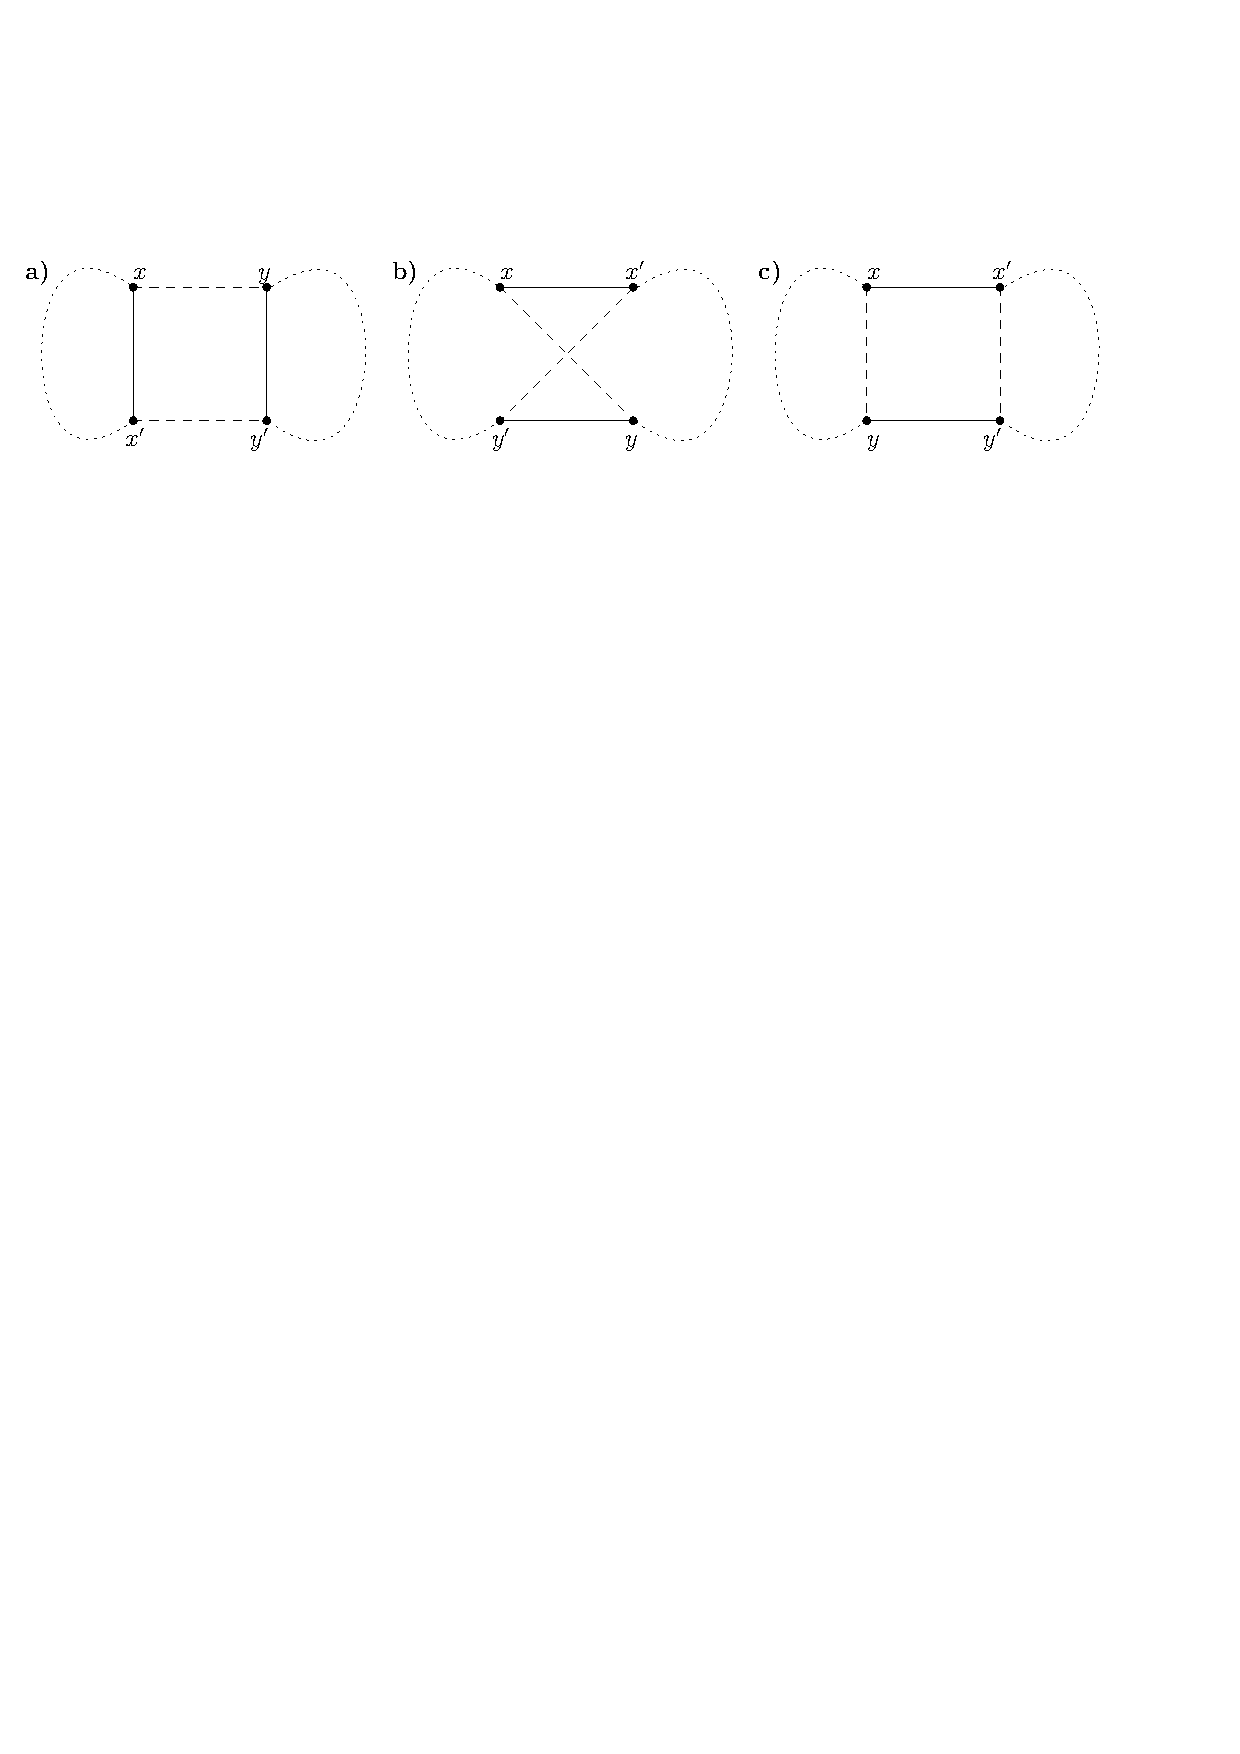
\includegraphics[width=0.95\textwidth]{figs/dynamic-mapping/fig_rematch}
\caption{Three cases in the analysis of the third stage (a swap performed by
\GREEDY). Solid edges denote edges that were removed from $\MGREEDY$ because
of the swap, dashed ones denote the ones that were added to $\MGREEDY$. Dotted
paths denote the remaining parts of the involved alternating cycle(s).}
\label{fig:rematch}
\end{figure}

\begin{enumerate}

\item
Assume that edges $(x,x')$ and $(y,y')$ were in different alternating
cycles before the swap, see \ref{fig:rematch}a. Then the number
of~alternating cycles decreases by one, and hence $\Delta \Psi = g \cdot
\alpha$. Let $C$ be the cycle that contained edge $(x,x')$. Node $x$ is adjacent
to an edge from $C$ that belongs to $\MOPT$. (It is possible that this edge is
$(x,x')$; this occurs in the degenerate case when $C$ is of length~$2$.) As
$\MOPT$ is a matching, $(x,y) \notin \MOPT$. Analogously, $(x',y') \notin
\MOPT$. Therefore, $\Phiinit(x,y) + \Phiinit(x',y') = f \cdot w(x,y) + f \cdot
w(x',y') = f \cdot \lambda \cdot \alpha$. Using the lemma assumption,
$\Delta \GREEDY + \sum_{e \in E} \Delta \Phi(e) + \Delta\Psi = (2 + g - f
\cdot \lambda) \cdot \alpha \leq 0$.

\item
Assume that edges $(x,x')$ and $(y,y')$ belonged to the same cycle and
it contained the nodes in the order $x,x',\ldots,y,y',\ldots$,
see~\ref{fig:rematch}b. In this case it holds that 
$\Delta \Psi = 0$, since 
the number of alternating cycles is unaffected by the swap. By similar
reasoning as in the previous case, neither $(x,y)$ nor $(x',y')$ belong to
$\MOPT$, and thus again, $\Phiinit(x,y) + \Phiinit(x',y') = f \cdot w(x,y) + f
\cdot w(x',y') = f \cdot \lambda \cdot \alpha$. In this case, $\Delta \GREEDY
+ \sum_{e \in E} \Delta \Phi(e) + \Delta\Psi = (2 - f \cdot \lambda) \cdot
\alpha \leq (2 + g - f \cdot \lambda) \cdot \alpha \leq 0$.

\item 
Assume that edges $(x,x')$ and $(y,y')$ belonged to the same cycle and
it contained the nodes in the order $x,x',\ldots,y',y,\ldots$,
see~\ref{fig:rematch}c. When the swap is performed, the number of
alternating cycles decreases, and thus $\Delta \Psi = -g \cdot \alpha$. Unlike
the previous cases, here it is possible that $(x,y)$ and $(x',y')$ belong to
$\MOPT$. But even in such a case, we may lower-bound the initial values of the
corresponding edge-potentials: $\Phiinit(x,y) + \Phiinit(x',y') \geq -
\winit(x,y) - \winit(x',y') = - \lambda \cdot \alpha$. Using the lemma
assumption, $\Delta \GREEDY + \sum_{e \in E} \Delta \Phi(e) + \Delta\Psi = (2
- g + \lambda) \cdot \alpha \leq 0$.
\end{enumerate}

\end{proof}




\begin{theorem}
\label{thm:rematching}
For $\lambda = 4/5$, $\GREEDY$ is $7$-competitive.
\end{theorem}

\begin{proof}
We choose $f = 6$ and $g = 14/5$. The chosen values of $\lambda$, $f$ and $g$
satisfy the conditions of \ref{lem:rematch_req},
\ref{lem:greedy_swap} and \ref{lem:opt_swap}. Summing these
inequalities over all stages occurring while serving an input sequence~$\sigma$
yields
\begin{equation*}
	\textstyle \GREEDY(\sigma) + (\Psi_\textrm{final} - \Psi_\textrm{initial})
	+ \sum_{e \in E} \left( 
		\Phi_\textrm{final}(e) - \Phi_\textrm{initial}(e) \right)
	\leq 7 \cdot \OPT(\sigma) \enspace,
\end{equation*}
where $\Psi_\textrm{final}$ and $\Phi_\textrm{final}(e)$ denote the final
values of the potentials and $\Psi_\textrm{initial}$ and
$\Phi_\textrm{initial}(e)$ their initial values. We observe that all the
potentials occurring in the inequality above are lower-bounded and
upper-bounded by values that are independent of the input sequence $\sigma$.
That is, $\Psi_\textrm{final} - \Psi_\textrm{initial} \geq - g \cdot \ell
\cdot \alpha$ (as the number of~alternating cycles is at most $\ell$) and
$\Phi_\textrm{final}(e) - \Phi_\textrm{initial}(e) \geq - (f+1) \cdot w(e)
\geq - (f+1) \cdot \lambda \cdot \alpha$ (as all edge weights are always 
at most $\lambda \cdot \alpha$). The number of edges is exactly $\binom{2
\cdot \ell}{2}$, and therefore
\begin{align*}
	 \GREEDY(\sigma) 
	\leq &\; 7 \cdot \OPT(\sigma) 
	+ \textstyle g \cdot \ell \cdot \alpha + \binom{2 \cdot \ell}{2} \cdot (f+1) \cdot 
	\lambda \cdot \alpha \\
	\leq &\; 7 \cdot \OPT(\sigma) 
	+ O(\ell^2 \cdot \alpha)
	\enspace.
\end{align*}
This concludes the proof.
\end{proof}


%%%%%%%%%%%%%%%%%%%%%%%%%%%%%%%%%%%%%%%%%%%%%%%%%%%%%%%%%%%%%%%%%%%%%%%%%%%%%%%%%
%%%%%%%%%%%%%%%%%%%%%%%%%%%%%%%%%%%%%%%%%%%%%%%%%%%%%%%%%%%%%%%%%%%%%%%%%%%%%%%%%

\section{Lower Bounds}
\label{sec:lower}

In order to shed light on the optimality of the presented online algorithm, we
next investigate lower bounds on the competitive ratio achievable by any
(deterministic) online algorithm. We start by showing a reduction of the BRP
problem to online paging, which will imply that already for two clusters the
competitive ratio of the problem is at least $k-1$. We strengthen this bound,
providing a lower bound of $k$ that holds for any amount of augmentation, as
long as the augmentation does not allow to put all nodes in a single 
cluster. The proof uses the averaging argument. We refine this approach for a
special case of online rematching ($k = 2$ without augmentation), for which we
present a~lower bound of $3$.


\subsection{Lower Bound by Reduction to Online Paging}
\label{sec:paging}

\begin{theorem}
Fix any $k$. If there exist a $\gamma$-competitive deterministic algorithm $B$
for BRP for two clusters, each of~size~$k$, then there exists a
$\gamma$-competitive deterministic algorithm $P$ for the paging problem with 
cache size $k-1$ and where the number of different pages is $k$.
\end{theorem}

\begin{proof}
The pages are denoted by $p_1,p_2,\ldots,p_k$. Without loss of generality, we
assume that the initial cache is equal to $p_1,p_2,\ldots,p_{k-1}$. We fix any
input sequence $\sigma^P = \sigma^P_1, \sigma^P_2, \sigma^P_3, \ldots$ for the
paging problem, where $\sigma^P_t$ denotes the $t$-th accessed page. We show
how to construct, in an online manner, an online algorithm $P$ for the paging
problem that operates in the following way. It internally runs the algorithm~$B$, 
starting on the initial assignment of nodes to clusters that will be
defined below. For a requested page $\sigma^P_t$, it creates a subsequence
of~communication requests for the BRP problem, runs $B$ on them, and serves
$\sigma^P_t$ on the basis of $B$'s responses.

We use the following $2k$ nodes for the BRP problem: paging nodes $p_1,p_2,
\ldots, p_k$, auxiliary nodes $a_1,a_2,\ldots,$ $a_{k-1}$, and a special node
$s$. We say that the node clustering is \emph{well aligned} if one cluster
contains the node $s$ and $k-1$ paging nodes, and the other cluster contains
one paging node and all auxiliary nodes. There is a natural bijection between
possible cache contents and well aligned configurations: the cache consists of
the $k-1$ paging nodes that are in the same cluster as node $s$. (Without loss
of generality, we may assume that the cache of any paging algorithm is always
full, i.e., consists of $k-1$ pages.) If the configuration $c$ of a BRP
algorithm is well aligned, $\textsc{cache}(c)$ denotes the corresponding cache
contents.

The initial configuration for the BRP problem is the well aligned
configuration corresponding to the initial cache (pages
$p_1,p_2,\ldots,p_{k-1}$ in the cache).

For any paging node $p$, let $\comm(p)$ be a subsequence of communication
requests for the BRP problem, consisting ot the request $(p, s)$, followed by
$\binom{k-1}{2}$ requests to all pairs of auxiliary nodes. Given an input
sequence $\sigma^P$ for online paging, we construct the input sequence
$\sigma^B$ for the BRP problem in the following way: For a request
$\sigma^P_t$, we repeat a~subsequence $\comm(\sigma^P_t)$ till the node
clustering maintained by $B$ becomes well aligned and $\sigma^P_t$ becomes
collocated with $s$. Note that $B$ must eventually achieve such a node
configuration: otherwise its cost would be arbitrarily large while a sequence
of repeated $\comm(\sigma^P_t)$ subsequences can be served at~a~constant
cost---the competitive ratio of~$B$ would then be unbounded. We denote the
resulting sequence of $\comm(\sigma^P_t)$ subsequences by
$\comm_t(\sigma^P_t)$.

To construct the response to the paging request $\sigma^P_t$, the algorithm
$P$ runs $B$ on $\comm_t(\sigma^P_t)$. Right after processing
$\comm_t(\sigma^P_t)$, node configuration $c$ of $B$ is well aligned and
$\sigma^P_t$ is collocated with~$s$. Hence, $P$ may change its cache
configuration to $\textsc{cache}(c)$: such a response is feasible because
since $\sigma^P_t$ is collocated with $s$, it is included by $P$ in the cache.
Furthermore, we may relate the cost of $P$ to the cost of~$B$: If $P$ modifies
the cache contents, the corresponding cost is $1$, as exactly one page has to
be fetched. Such a change occurs only if $B$ changed node placement in
clusters (at a~cost of at least $2 \cdot \alpha$). Therefore, $2
\cdot \alpha \cdot P(\sigma^P_t) \leq B(\comm_t(\sigma^P_t))$, which
summed over all requests from sequence $\sigma^P$ yields $2 \cdot
\alpha \cdot P(\sigma^P) \leq B(\sigma^B)$.

Now we show that there exists an (offline) solution \OFF to $\sigma^B$, whose
cost is exactly $2 \cdot \alpha \cdot \OPT(\sigma^P)$. Recall that, for a
paging request $\sigma^P_t$, $\sigma^B$ contains the~corresponding sequence
$\comm_t(\sigma^P_t)$. Before serving the first request
of~$\comm_t(\sigma^P_t)$, \OFF changes its state to a well aligned
configuration corresponding to the cache of $\OPT$ right after serving paging
request $\sigma^P_t$. This ensures that the subsequence $\comm_t(\sigma^P_t)$
is free for \OFF. Furthermore, the cost of node migration of \OFF is $2
\alpha$ (two paging nodes are swapped) if $\OPT$ performs a fetch, and 0 if
$\OPT$ does not change its cache contents. Therefore,
$\OFF(\comm_t(\sigma^P_t)) = 2 \cdot \alpha \cdot \OPT(\sigma^P_t)$, which
summed over the entire sequence $\sigma^P$ yields $\OFF(\sigma^B) = 2 \cdot
\alpha \cdot \OPT(\sigma^P)$.

As $B$ is $\rho$-competitive for the BRP problem, there exists a constant
$\beta$, such that for any sequence $\sigma^P$ and the corresponding sequence
$\sigma^B$, it holds that $B(\sigma^B) \leq \gamma \cdot \OPT(\sigma^B) +
\beta$. Combining this inequality with proven relations between $P$ and $B$
and between \OFF and \OPT yields
\[
	2 \cdot \alpha \cdot P(\sigma^P) \leq 
	B(\sigma^B) \leq \gamma \cdot \OPT(\sigma^B) + \beta
	\leq \gamma \cdot \OFF(\sigma^B) + \beta
	 =\gamma \cdot 2 \cdot \alpha \cdot \OPT(\sigma^P) + \beta
	\enspace,
\]
and therefore $P$ is $\gamma$-competitive.
\end{proof}

As any deterministic algorithm for the paging problem with cache size $k-1$
has a competitive ratio of~at~least $k-1$~\cite{SleTar85}, we obtain the
following result.

\begin{corollary}
The competitive ratio of the BRP problem on two clusters is at least $k-1$. 
\end{corollary}


\subsection{Additional Lower Bounds}
\label{sec:lower-bounds}

\begin{theorem}\label{thm:loweraugmk}
No~$\delta$-augmented deterministic online algorithm \ONL
can achieve a competitive ratio smaller than~$k$, as long as~$\delta < \ell~$.
\end{theorem}

\begin{proof}
In our construction, all nodes are numbered from $v_0$ to $v_{n-1}$. All
presented requests are edges in~a~ring graph on these nodes with edge $e_i$
defined as $(v_i,v_{(i+1) \mod n })$ for~$i = 0, \ldots, n-1$. At any time,
the adversary gives a communication request between an arbitrary pair of nodes
not collocated by \ONL. As $\delta < \ell$, \ONL cannot fit the entire ring in
a single cluster, and hence such pair always exists. Such a request
entails a cost of~at~least~$1$ for \ONL. This way, we may define an~input
sequence $\sigma$ of an~arbitrary length, such that $\ONL(\sigma) \geq
|\sigma|$.

Now we present $k$ offline algorithms $\OFF_1, \OFF_2, \ldots, \OFF_k$, such
that, neglecting an initial node reorganization that they will perform before
the input sequence starts, the sum of their total costs on $\sigma$ is exactly
$|\sigma|$. Toward this end, for any $j \in \{0,\ldots,k-1\}$, we define a~set $\cut(j) = \{ e_j, e_{j+k}, e_{j+2k},
\ldots, e_{j+(\ell-1)\cdot k} \}$. For any~$j$, set $\cut(j)$ defines a
natural partitioning of all nodes into clusters, each containing $k$ nodes.
Before processing $\sigma$, the algorithm $\OFF_j$ first migrates its nodes
(paying at most $n \cdot \alpha$) to the clustering defined by $\cut(j)$ and
then never changes the node placement.

As all sets $\cut(j)$ are pairwise disjoint, for any request $\sigma_t$,
exactly one algorithm $\OFF_j$ pays for the request, and thus $\sum_{j=1}^k
\OFF_j(\sigma_t) = 1$. Therefore, taking the initial node reorganization into
account, we obtain that $\sum_{j=1}^k \OFF_j(\sigma) \leq k \cdot n \cdot
\alpha + \ONL(\sigma)$. By the averaging argument, there exists offline
algorithm $\OFF_j$, such that $\OFF_j(\sigma) \leq \frac{1}{k} \cdot
\sum_{j=1}^k \OFF_j(\sigma) \leq n \cdot \alpha + \ONL(\sigma) / k$.
Thus, $\ONL(\sigma) \geq k \cdot \OFF_j(\sigma) - k \cdot n \cdot
\alpha \geq k \cdot \OPT(\sigma) - k \cdot n \cdot \alpha$.
The~theorem follows because the additive constant $k \cdot n \cdot \alpha$
becomes negligible as the length of $\sigma$ grows.
\end{proof}


\begin{theorem}
No deterministic online algorithm \ONL can achieve a competitive ratio 
smaller than~$3$ for the case $k = 2$ (without augmentation).
\end{theorem}

\begin{proof} As in the previous proof, we number the nodes from $v_0$ to
$v_{n-1}$. We distinguish three types of node clusterings. Configuration A:
$v_0$ collocated with $v_1$, $v_2$ collocated with $v_3$, other nodes
collocated arbitrarily; configuration B: $v_1$ collocated with $v_2$, $v_3$
collocated with $v_0$, other nodes collocated arbitrarily; configuration C:
all remaining clusterings.

Similarly to the proof of \ref{thm:loweraugmk}, the adversary always
requests a communication between two nodes not collocated by \ONL.
This time the exact choice of such nodes is relevant: \ONL receives request to
$(v_1,v_2)$ in configuration A, and to $(v_0,v_1)$ in configurations B and C.

We define three offline algorithms. They will keep nodes
$\{v_0,\ldots,v_3\}$ in the first two clusters and the remaining nodes in the
remaining clusters (the remaining nodes will never change their clusters). 
More concretely, $\OFF_1$ keeps nodes $\{v_0,\ldots,v_3\}$ always in
configuration A and $\OFF_2$ always in configuration B. Furthermore, we define
the third algorithm $\OFF_3$ that is in configuration B if \ONL is in
configuration A, and is in configuration A if \ONL is in configuration B or C.

We split the cost of $\ONL$ into the cost for serving requests, $\ONLreq$, and
the cost paid for its migrations, $\ONLmig$. Observe that, for~any~request
$\sigma_t$, $\OFF_1(\sigma_t) + \OFF_2(\sigma_t) = \ONLreq(\sigma_t)$.
Moreover, as $\OFF_3$ does not pay for any request and migrates at the same
time as \ONL does, $\OFF_3(\sigma_t) = \ONLmig(\sigma_t)$. Summing up,
$\sum_{j=1}^3 \OFF_j(\sigma_t) = \ONL(\sigma_t)$ for any request $\sigma_t$.
Taking into account the initial reconfiguration of nodes in $\OFF_j$ solutions
(which involves at~most one swap of cost $2 \cdot \alpha$), we obtain that
$\sum_{j=1}^3 \OFF(\sigma) \leq 2 \cdot \alpha + \ONL(\sigma)$. Hence, by the
averaging argument, there exists $j \in \{1,2,3\}$, such that $\ONL(\sigma)
\geq 3 \cdot \OFF_j(\sigma) - 2 \cdot \alpha \geq 3 \cdot \OPT(\sigma) - 
2 \cdot \alpha$. This concludes the proof, as $2 \cdot \alpha$ becomes
negligible as the length of $\sigma$ grows.
\end{proof}

\section{Conclusions}\label{sec:conclusion-dynamic}

\todo{TODO: empty}

\part{Memory management in network devices / or: cache management in network devices / or: managing resources in network devices}

\chapter{Optimizing routing tables}


In this chapter, we introduce a natural extension of an online paging problem, where
items have inter-de\-pen\-den\-cies.
In the classic online paging problem, items of some universe are requested by
a~processing entity (e.g., blocks of RAM are requested by the processor). To
speed up the access, computers use a faster memory, called
\emph{cache}, capable of accommodating $k$ such items. Upon a~request to a
non-cached item, the algorithm has to fetch it into the cache, paying a fixed
cost, while a request to a cached item is free. If the cache is full, the
algorithm has to free some space by evicting an arbitrary subset of items from
the cache.
%The model variant, where fetching is optional (the requested item can be served without being in the cache, incurring some fixed cost) is called a \emph{bypassing model}.
In the traditional caching problem, the cache elements are independent: it is always feasible to pull in or out the elements of the cache regardless of cache configuration.



Dependencies among to-be-cached items arise in numerous settings and are a
natural refinement of many caching problems.
As highlighted in the introduction, an important application for caching with tree-based dependency model arises in the context
of forwarding rules in routers. We begin by a technical overview, %in Section~\ref{sec:tc-technical},
where we explain the the setup for \emph{caching of forwarding rules} in a router.
Then, we introduce the formal model for caching with hierarchical dependencies, for which we propose a competitive algorithm.
In Section~\ref{sec:bisimulation} we establish a connection between caching with hierarchical dependencies and caching of forwarding rules.
Finally, we show that the proposed algorithm can be efficiently implemented.


%Nowadays, routers have to store an~enormous number of forwarding rules: the
%number of rules has doubled in the last six years~\cite{bgp-routeviews} and
%the superlinear growth is likely to be sustained~\cite{steve-myth}. This
%entails large costs for Internet Service Providers: fast router memory
%(usually Ternary Content Addressable Memory (TCAM)) is expensive and
%power-hungry~\cite{tcam-expensive}.  Many routers currently either operate at
%(or beyond) the edge of their memory capacities. A~solution, which could delay
%the need for expensive or impossible memory upgrades in routers, is to store
%only a subset of rules in the actual router and store all rules on a~secondary
%device (for example a commodity server with a large but slow
%memory)~\cite{cacheflow,route-caching-flat,prefix-caching,fib-caching-non-overlapping,fibium-zipf}.

%In Section~\ref{sec:tc-technical} we present the technical setup for our proposed solution,
%then in Section~\ref{sec:preliminaries} we present the formal model, and in Section~\ref{}.
%In Section~\ref{sec:preliminaries} we present the formal model for studying the caching problem with dependencies that we call Online Tree Caching, and 
%in Section~\ref{sec:algo} we propose the algorithm \ALGTC for this model.
%In Section~\ref{sec:analysis}, we show that \ALGTC is competitive 
%In Section~\ref{sec:implementing_counters}, we show how \ALGTC can be efficiently implemented.
%We start by presenting the technical setup (FIB caching) for our proposed solution in Section~\ref{sec:tc-technical}, and in Section~\ref{sec:bisimulation}, we show the reduction that allows to use solution for Online Tree Caching to solve the FIB caching.

\section{Technical Setup}
\label{sec:tc-technical}

\begin{figure}[t]
\centering
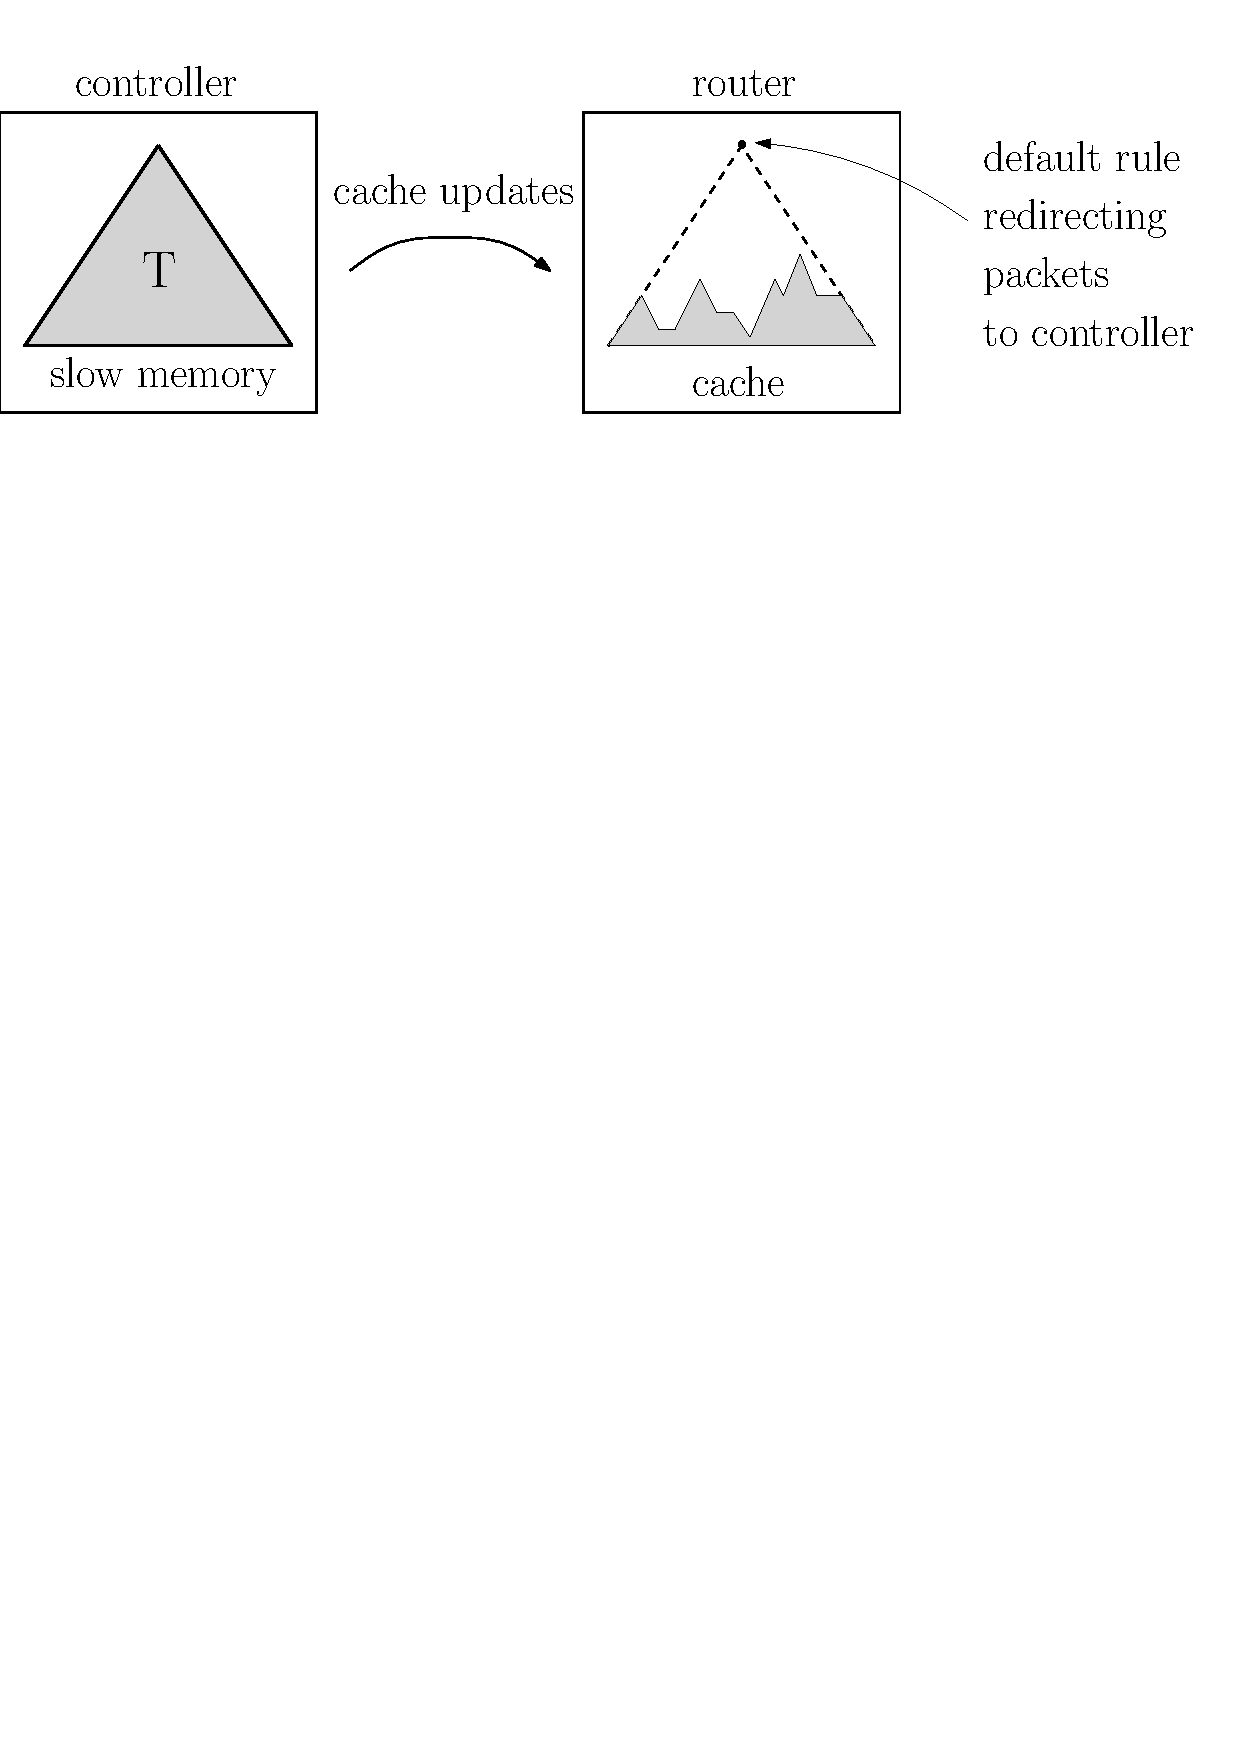
\includegraphics[width=0.7\columnwidth]{figs/cache-management/router.pdf}
\caption{The router (\emph{right}) caches only a subset of all rules, and
  rules that are not cached are answered by the controller (\emph{left}) that
  keeps the whole tree of rules. Updates to the rules are passed by the
  controller to the router.}\label{fig:router}
\end{figure}

As highlighted in the introduction, routers has finite memory, and in an increasingly common scenario the size of forwarding table exceeds the size of available memory.
One of the solutions is to store only a part of a~forwarding table on the router, that acts as a cache for the complete forwarding table.
The setup  depicted in
\lref[Figure]{fig:router} consists of two entities: a single router 
(e.g., an OpenFlow switch) which caches only a~subset of all forwarding rules,
and the (SDN) controller, which keeps all rules in its less expensive and
slower memory (see~\cite{fibium-zipf} for a more technical discussion). During runtime, packets arrive at the router, and if an
appropriate forwarding rule is found within the rules cached by the router,
then the packet is forwarded accordingly, and the associated cost is zero.
Otherwise, the packet has to be forwarded to the controller (where 
an~appropriate forwarding rule exists); this indirection costs~$1$. Hence, the
rules correspond to cacheable items and accesses to rules are modeled by
positive requests to the corresponding items. At some chosen points in time,
the caching algorithm run at the controller may decide to remove or add rules
to the cache. Any such change entails a~fixed cost $\alpha$.\footnote{This
cost corresponds to the transmission of a message from the controller to the
router as well as the update of internal data structures of the router. Such
an update of proprietary and vendor-dependent structures can be quite
costly~\cite{tcam-expensive-updates}, but the empirical studies show it to be
independent of the rule being updated~\cite{fib-updates}.}

Additionally, a rule may need to be updated. For example, due to a~change
communicated by a dynamic routing protocol (e.g., BGP) the action defined by
a~rule has to be modified. In either case, we have to update the rules at the
controller: we assume that this cost is zero. (This cost is unavoidable for
any algorithm, so such an assumption makes our problem only more difficult.)
Furthermore, if the rule is also stored at the router, then we have to pay a~fixed
cost of $\alpha$ for updating the router (we will show that such penalties can be easily simulated in our model, see Section~\ref{sec:bisimulation}).


The forwarding table consists of rules that might be nested, and hence its structure is hierarchical.
The forwarding rules are prefixes of
IP addresses (they are bit strings). Whenever a packet arrives, the router
follows a longest matching prefix (LMP) scheme: it searches for the rule that
is a~prefix of the destination IP of the packet and among matching rules it
chooses the longest one. In other words, if the prefixes corresponding to
rules are stored in the tree\footnote{We do not have to assume that they are
actually stored in a real tree; this tree is implicit in the LMP scheme.},
then the tree is traversed from the root downwards, and the last found rule is
used.
Similarly to forwarding rules, in our model the cached nodes to form a subforest:
leaving a less specific rule on the router while evicting a more specific one
(i.e., keeping a~tree node in cache while evicting its descendant) will result
in a~situation where packets will be forwarded according to the less specific
rule, and hence potentially exit through the wrong port.

In the proposed scenario, a situation may occur, where that the router does not have sufficient information to proceed.
The common way to handle the situation is to redirect the packet to the controller, which keeps the copy of the complete forwarding table.
However, the packet cannot be forwarded by the controller, hence it is supplemented with forwarding informations and sent back to the router.
Then, the router overrides the usual procedure of forwarding table lookup, and instead it uses the supplemented information to forward the packet.
Note that the described approach is implementable: one could simply add
an~artificial rule at the tree root in the router (matching an empty prefix).
This ensures that when no actual matching rule is found in the router (in the
cache), the packet will be forwarded according to this artificial rule to the
control plane that stores all the rules and can handle all packets appropriately.


Following this situation, the control plane may decide to update the cached portion of the forwarding table kept in the forwarding component.
Standard caching-related problems arise, such as: which entry to evict to provide space to store the new one.
Immediate update might seem a rational strategy, but in scenarios with highly dynamic networks that rearrange often, it might be beneficial to delay the update.
Premature update might result in the situation, where more time is spent alternating the cache configuration than processing packets (this is similar to \emph{thrashing} in virtual memory systems).

The proposed solution is particularly attractive with the advent of Soft\-ware-Defined
Network (SDN) technology, which allows to manage the expensive memory using a
software controller~\cite{cacheflow,fibium-zipf}. In particular, our
theoretical model can describe real-world architectures
like~\cite{cacheflow,fibium-zipf},
that is, our model formalizes the underlying operational
problems of such architectures. Our 
algorithm, when applied in the context of such architectures, can 
hence be used to prolong the lifetime of IP routers.



\section{Problem Definition}\label{sec:preliminaries}

%In the classic online paging problem, items of some universe are requested by
%a~processing entity (e.g., blocks of RAM are requested by the processor). To
%speed up the access, computers use a faster memory, called
%\emph{cache}, capable of accommodating $k$ such items. Upon a~request to a
%non-cached item, the algorithm has to fetch it into the cache, paying a fixed
%cost, while a request to a cached item is free. If the cache is full, the
%algorithm has to free some space by evicting an arbitrary subset of items from
%the cache.
%
%The paging problem is inherently online: the algorithm has to make decisions
%what to evict from the cache without the knowledge of future requests; its
%cost is compared to the cost of an optimal \emph{offline} solution and the
%worst-case ratio of these two amounts is called \emph{competitive ratio}. The first
%analysis of this basic problem in an online model was given over three
%decades ago by Sleator and Tarjan~\cite{competitive-analysis}. The problem was later
%considered in a~variety of flavors. In particular, some papers considered a
%\emph{bypassing model}~\cite{caching-rejection-penalties,paging-irani}, where
%item fetching is optional: the requested item can be served without being in
%the cache, for another fixed cost (usually being at most the cost of item
%fetching).

In our model, we assume that the universe is
an arbitrary (not necessarily binary) rooted tree $T$ and the requested items
are its nodes. For any tree node $v$, $T(v) \subseteq T$ is a subtree rooted
at $v$ containing $v$ and all its descendants. We require the following
property: if a~node $v$ is in the cache, then all nodes of $T(v)$ are also
cached. In other words, we require that \emph{the cache is a~subforest of
$T$}, i.e., a union of disjoint subtrees of~$T$.  We call this problem
\emph{online tree caching}.

We assume discrete time slotted into rounds, with round $t \geq 1$
corresponding to time interval $(t-1,t)$. In round $t$, the algorithm is given
one (positive or negative) request to exactly one tree node and has to process
it, i.e., pay associated costs (if any). 
Furthermore, we assume a bypassing model and distinguish between two types of
requests: a~request can be either \emph{positive} or \emph{negative}. The
positive requests correspond to ``normal'' requests known from caching
problems: we pay~$1$ if the node is not cached; for a negative request, we pay
$1$ if the corresponding request is cached.

After serving the request, we may
reorganize our cache arbitrarily, but the resulting cache has to still be a
subforest of $T$. We pay $\alpha$ for fetching or evicting any single node,
where $\alpha \geq 1$ is an integer and a~parameter of the problem. Our goal
is to minimize the overall cost of maintaining the cache and serving the
requests.

Right after round~$t$, at time $t$,
the algorithm may arbitrarily reorganize its cache, (i) ensuring that the
resulting cache is a subforest of $T$ (i.e., if the cache contains node $v$,
then it contains the entire~$T(v)$) and (ii)~preserving the cache capacity
constraint. An algorithm pays $\alpha$ for a~single node fetch or eviction. We
denote the contents of the cache at round $t$ by $C_t$. (As the cache changes
contents only between rounds, $C_t$ is well defined.) We assume that $\alpha$
is an even integer (this assumption may change costs at most by a constant
factor). We assume that the algorithm starts with the empty cache.
%%%%%%%%%%%%%%%%%%%%%%%%%%%%%%%%%%%%%%%%%%%%%%%%%%%%%%%%%%%%%%%%%%%%%%%%%%%%%%%%%%%
%%%%%%%%%%%%%%%%%%%%%%%%%%%%%%%%%%%%%%%%%%%%%%%%%%%%%%%%%%%%%%%%%%%%%%%%%%%%%%%%%%%

\section{Algorithm TC}\label{sec:algo}

The algorithm \textsc{Tree Caching} (\ALGTC) presented in the following is
a simple scheme that follows a \emph{rent-or-buy paradigm}: it fetches (or evicts)
a changeset $X$ if the cost associated with requests at $X$ reaches the cost of 
such fetch or eviction.
More concretely, \ALGTC operates in multiple phases. The first phase starts at time $0$.
\ALGTC starts each phase with the empty cache and proceeds as follows. Within a
phase, every node keeps a~counter, which is initially zero. If at round~$t$ it
pays~$1$ for serving the request, it increments its counter. Whenever a node
is fetched or evicted from the cache, its counter is reset to zero. Note that
this implies that the counter of $v$ is equal to the number of negative
(positive) requests to $v$ since its last fetching to the cache (eviction from
the cache). For a~set $A \subseteq T$, we denote the sum of all counters in
$A$ at time $t$ by $\cnt_t(A)$.

We call a non-empty set $X$ a \emph{valid positive changeset} for cache $C$ if
$X \cap C = \emptyset$ and $C \cup X$ is a subforest of~$T$, and a~\emph{valid
negative changeset} if $X \subseteq C$ and $C \setminus X$ is a subforest of
$T$. We call $X$ a~\emph{valid changeset} if it is either valid positive or
negative changeset. Note that the union of positive (negative) changesets is
also a valid positive (negative) changeset. We say that the algorithm applies
changeset~$X$, if it fetches all nodes from~$X$ (for a positive changeset) and
evicts all nodes from $X$ (for a negative one). Note that not all valid
changesets may be applied as the algorithm is also limited by its cache capacity
($\kALG$ for an online algorithm and $\kOPT$ for the optimal offline one).


At time~$t$, \ALGTC verifies whether
there exists a~valid changeset $X$, such that
\begin{itemize}
\item \emph{(saturation property)} $\cnt_t(X) \geq |X| \cdot \alpha$ and
\item \emph{(maximality property)} $\cnt_t(Y) < |Y| \cdot \alpha$ for any valid
  changeset $Y \supsetneq X$.
\end{itemize}
In this case, the algorithm modifies its cache applying~$X$. 
If, at time $t$, \ALGTC is supposed to fetch some set $X$, but by doing so it
would exceed the cache capacity $\kALG$, it evicts all nodes from the cache
instead, and starts a~new phase at time~$t$. Such a \emph{final eviction}
might not be present in the last phase, in which case we call it
\emph{unfinished}. 


In \lref[Lemma]{lem:no_over-requested_changesets} (below), we show that at any
time, all valid changesets satisfying both properties of \ALGTC are either all
positive or all negative. Furthermore, right after the algorithm applies a
changeset, no valid changeset satisfies saturation property.

%%%%%%%%%%%%%%%%%%%%%%%%%%%%%%%%%%%%%%%%%%%%%%%%%%%%%%%%%%%%%%%%%%%%%%%%%%%%%%%%%%%
%%%%%%%%%%%%%%%%%%%%%%%%%%%%%%%%%%%%%%%%%%%%%%%%%%%%%%%%%%%%%%%%%%%%%%%%%%%%%%%%%%%


\section{Analysis}
\label{sec:analysis}

We denote the height of $T$ by $h(T)$.  A
\emph{tree cap} rooted at $v$ is ``an~upper part'' of $T(v)$, i.e., it
contains $v$ and if it contains node~$u$, then it also contains all nodes on
the path from $u$ to $v$. If $A \subseteq B$ are both tree caps rooted at $v$,
then we say that $A$ is a tree cap of $B$.


Throughout this chapter, we fix an input $I$, its partition into phases, and
analyze both \ALGTC and \OPT on a~single fixed phase $P$. We denote the times at
which $P$ starts and ends by $\beP$ and $\enP$, respectively, i.e., rounds in
$P$ are numbered from $\beP+1$ to $\enP$. A proof of the following technical
lemma follows by induction and is presented in 
\lref{sec:proof_of_lemma_1}.


\begin{lemma}
\label{lem:no_over-requested_changesets}
Fix any time $t > \beP$. For any valid changeset $X$ for $C_t$, it holds that
$\cnt_t(X) \leq |X| \cdot \alpha$. If a~changeset $X$ is applied at time $t$,
the following properties hold:
\begin{enumerate}
\item $X$ contains the node requested at round $t$, 
\label{lemit:1}
\item $\cnt_t(X) = |X| \cdot \alpha$, 
\label{lemit:2}
\item $\cnt_t(Y) < |Y| \cdot \alpha$ for any valid changeset $Y$ for~$C_{t+1}$
(note that $C_{t+1}$ is the cache state right after application of $X$),
\label{lemit:3}
\item $X$ is a tree cap of a tree from $C_{t+1}$ if
$X$ is positive and it is a~tree cap of a tree from $C_t$ if $X$ is
negative.
\label{lemit:4}
\end{enumerate}
\end{lemma}

In the following, we assume that no positive requests are given to nodes
inside cache and no negative ones to nodes outside of it. (This does not
change the behavior of \ALGTC and can only decrease the cost of \OPT.)

For the sake of analysis, we assume that at time $\enP$, \ALGTC actually
performs a cache fetch (exceeding the cache size limit) and then, at the same
time instant, empties the cache. This replacement only increases the cost of
\ALGTC. Let $k_P$ denote the number of nodes in the cache of $\ALGTC$ at $\enP$.
In a finished phase, we measure it after the artificial fetch, but right
before the final eviction, and thus $k_P \geq \kALG + 1$; in an unfinished
phase $k_P \leq \kALG$.

The crucial part of our analysis that culminates in
\lref[Section]{sec:shifting} is the technique of shifting requests. Namely, we
modify the input sequence by shifting requests up or down the tree, so that
the resulting input sequence (i) is not harder for \OPT and (ii) is more
structured: we may lower bound the cost of \OPT on each node separately and
relate it to the cost of \ALGTC.


%%%%%%%%%%%%%%%%%%%%%%%%%%%%%%%%%%%%%%%%%%%%%%%%%%%%%%%%%%%%%%%%%%%%%%%%%%%%%%%%%%%
%%%%%%%%%%%%%%%%%%%%%%%%%%%%%%%%%%%%%%%%%%%%%%%%%%%%%%%%%%%%%%%%%%%%%%%%%%%%%%%%%%%

\subsection{Event Space and Fields}
\label{sec:event}

In our analysis, we look at a two-dimensional, discrete, spatial-temporal
space, called the \emph{event space}. The first dimension is indexed by tree
nodes, whose order is an~arbitrary extension of the partial order given by the
tree. That is, the parent of a node $v$ is always ``above''~$v$. The second
dimension is indexed by round numbers of phase~$P$. The space elements are
called \emph{slots}. Some slots are occupied by requests: a~request at node
$v$ given at round $t$ occupies slot $(v,t)$. From now on, we will identify
$P$ with a set of requests occupying some slots in the event space.

We partition slots of the whole event space into disjoint parts, called
\emph{fields}, and we show how this partition is related to the costs of \ALGTC
and \OPT. For any node~$v$ and time $t$, $\last_v(t)$ denotes the last time
strictly before~$t$, when node $v$ changed state from cached to non-cached or
vice versa; $\last_v(t) = \beP$ if $v$ did not change its state before $t$ in
phase $P$. For a~changeset~$X_t$ applied by
\ALGTC at time $t$, we define the field $F^t$ as
\[
  F^t = \left\{\ (v,r) : v \in X_t \, \wedge\, \last_v(t)+1 \leq r \leq t\ \right\}.
\]
That is, field $F^t$ contains all the requests that eventually trigger the
application of $X_t$ at time $t$. We say that $F^t$ ends at $t$. We call field
$F^t$ \emph{positive} (\emph{negative}) if $X_t$ is a positive (negative)
changeset. An~example of a~partitioning into fields is given in
\lref[Figure]{fig:fields}. We define $\req(F^t)$ as the number of requests
belonging to slots of~$F^t$ and let $\sizetc(F^t)$ be the number of involved
nodes (note that $\sizetc(F^t) = |X_t|)$. The observation below follows
immediately by \lref[Lemma]{lem:no_over-requested_changesets}.

\begin{figure}[t]
  \centering
  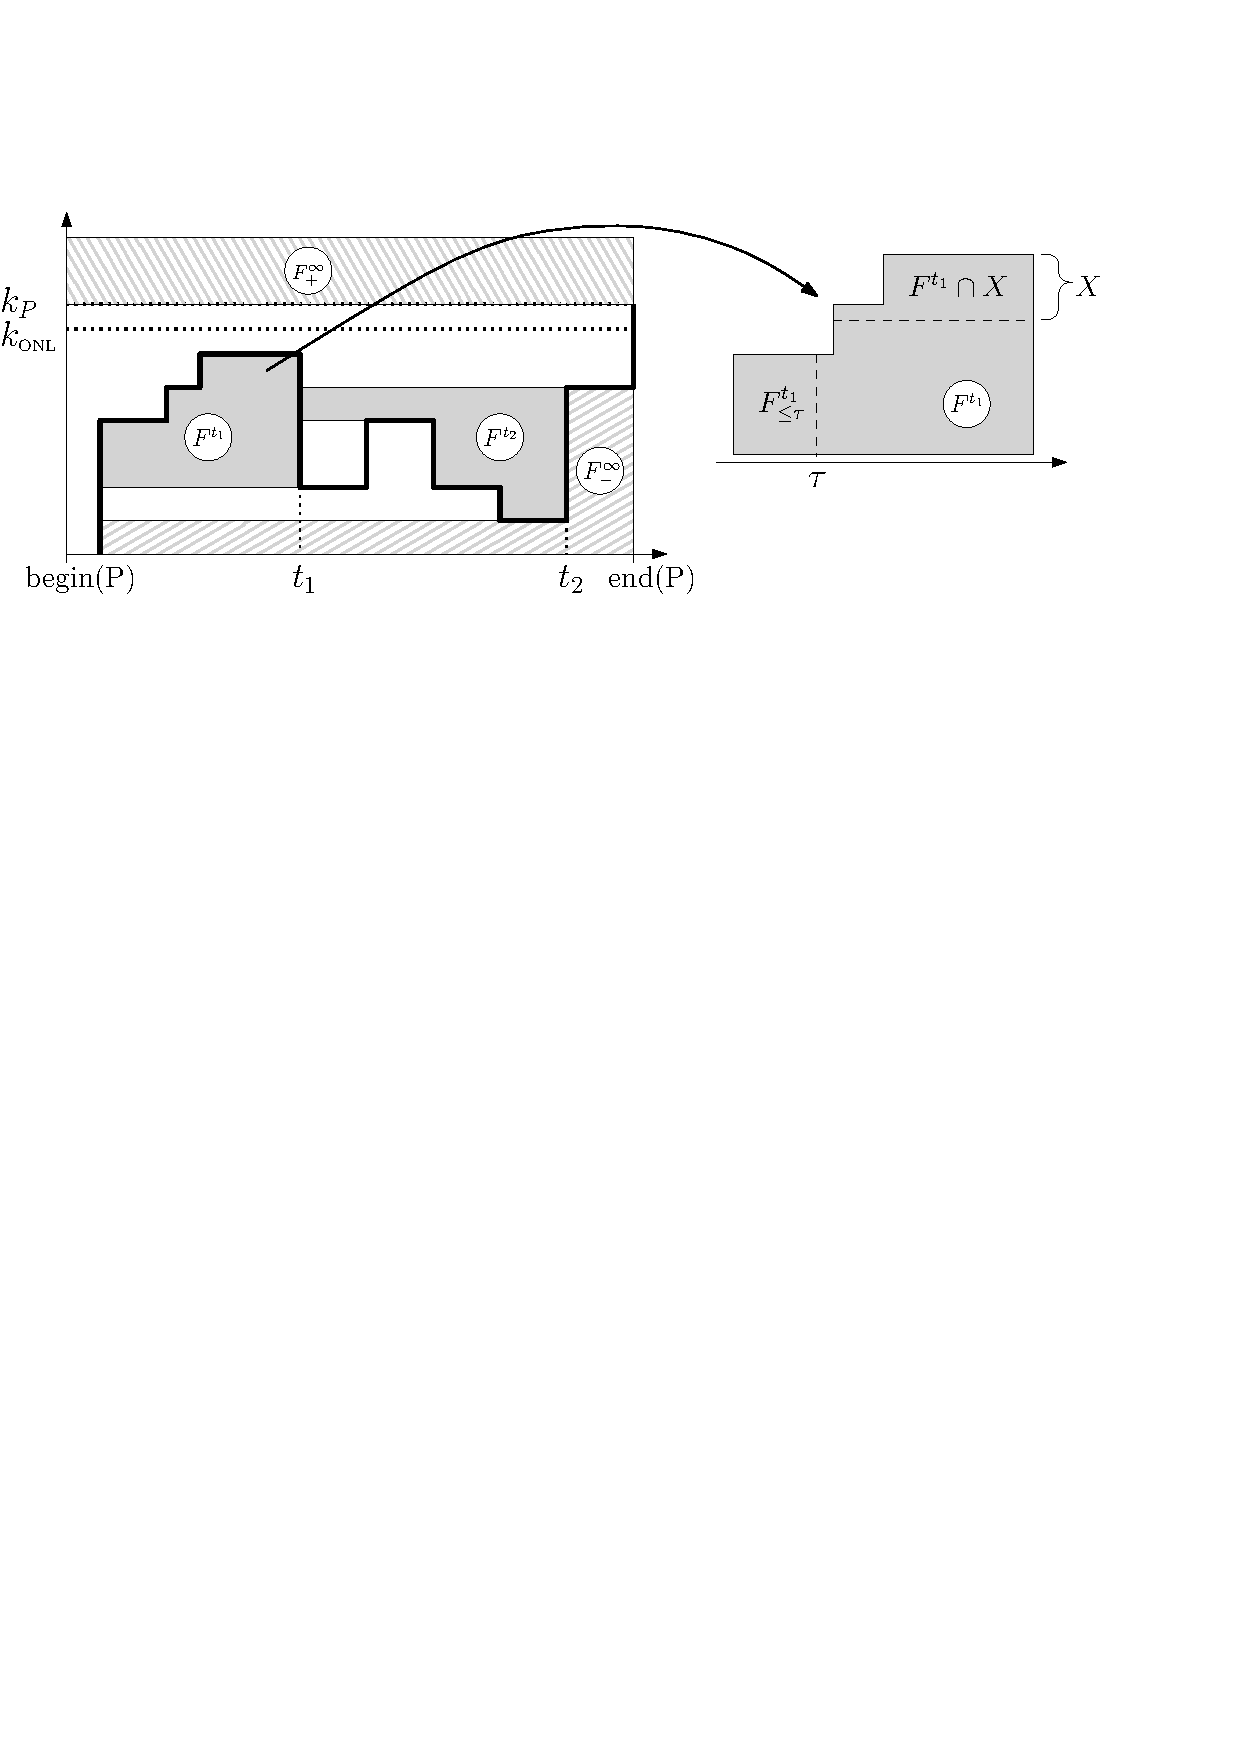
\includegraphics[width=0.99\columnwidth,keepaspectratio]{figs/cache-management/fields_horizontal}
  \caption{Partitioning of a single phase into fields for a line (a tree with
  no branches). The thick line represents cache contents. Possible final eviction
  at $\enP$ is not depicted. $F^{t_1}$ is a~negative field and $F^{t_2}$ is a
  positive one. In the particular depicted example, nodes are ordered from the
  leaf (bottom) to the root (top  of the picture). We emphasize that for a
  general, branched tree, some notions (in particular fields) no longer have
  nice geometric interpretations.}
  \label{fig:fields}
\end{figure}


\begin{observation}
\label{obs:field_requests}
For any field $F$, $\req(F) = \sizetc(F) \cdot \alpha$. All these requests are
positive (negative) if $F$ is positive (negative).
\end{observation}

Finally, we call the rest of the event space defined by phase $P$
\emph{open field} and denote it by $F^\infty$. The set of all fields except $
F^\infty$ is denoted by $\F$. Let $\sizetc(\F) = \sum_{F \in \F} \sizetc(F)$.

\begin{lemma}
\label{lem:alg_cost}
For any phase $P$ partitioned into a set of fields $\F \cup \{ F^\infty \}$,
it holds that $\ALGTC(P) \leq 2 \alpha \cdot \sizetc(\F) + \req(F^\infty) + k_P
\cdot \alpha$.
\end{lemma}

\begin{proof}
By \lref[Observation]{obs:field_requests}, the cost associated with serving
the requests from all fields from $\mathcal{F}$ is $\sum_{F \in \F} \alpha
\cdot \sizetc(F) = \alpha \cdot \sizetc(\F)$. The cost of the cache reorganization
at the fields' ends is exactly the same. The term $\req(F^\infty)$ represents
the cost of serving the requests from $F^\infty$ and $k_P \cdot \alpha$
upper-bounds the cost of the final eviction (not present in an unfinished
phase).
\end{proof}



%%%%%%%%%%%%%%%%%%%%%%%%%%%%%%%%%%%%%%%%%%%%%%%%%%%%%%%%%%%%%%%%%%%%%%%%%%%%%%%%%%%
%%%%%%%%%%%%%%%%%%%%%%%%%%%%%%%%%%%%%%%%%%%%%%%%%%%%%%%%%%%%%%%%%%%%%%%%%%%%%%%%%%%

\subsection{Shifting Requests}\label{sec:shifting}

The actual challenge in the proof is to relate the structure of the fields to
the cost of {\OPT}. The rationale behind our construction is based on the
following thought experiment. Assume that the phase is unfinished (for
example, when the cache is so large that the whole input corresponds to a
single phase). Recall that the number of requests in each field $F \in \F$ is
equal to $\sizetc(F) \cdot \alpha$. Assume that these requests are evenly
distributed among the nodes of $F$ (each node from $F$ receives $\alpha$
requests in the slots of $F$). Then, the history of any node $v$ is
alternating between periods spent in positive fields and periods spent in
negative fields. By our even distribution assumption, each such a period
contains exactly $\alpha$ requests. Hence, for any two consecutive periods of
a~single node, \OPT has to pay at least $\alpha$ (either $\alpha$ for positive
requests or $\alpha$ for negative ones, or $\alpha$ for changing the
cached/non-cached state of $v$). Essentially, this shows that $\OPT$ has to
pay an amount that can be easily related to $\alpha \cdot
\sizetc(\F)$.

Unfortunately, the requests may not be evenly distributed among the nodes. To
alleviate this problem, we will modify the requests in phase $P$, so that the
newly created phase $P'$ is not harder for $\OPT$ and will ``almost'' have the
even distribution property. In this construction, the time frame of $P$ and
its fields are fixed.

\subsubsection{Legal Shifts}

We say that a request placed originally (in phase $P$) at slot $(v,t)$ is
\emph{legally shifted} if its new slot is $(m(v), t)$, where (i) for a
positive request, $m(v)$ is either equal to~$v$ or is one of its descendants
and (ii) for a negative request, $m(v)$ is either equal to $v$ or is one of
its ancestors. For any fixed sequence of fetches and evictions within phase
$P$, the associated cost may only decrease when these actions are replayed on
the modified requests.

\begin{observation}
\label{obs:pprim_easier_than_p}
If $P'$ is created from $P$ by legally shifting the requests, then $\OPT(P')
\leq \OPT(P)$.
\end{observation}

The main difficulty is however in keeping the legally shifted requests within
the field they originally belonged to. For example, a negative request from
$F$ shifted at round $t$ from node~$u$ to its parent may fall out of $F$ as
the parent may still be outside the cache at round~$t$. In effect, a careless
shifting of requests may lead to a situation where, for a single node~$v$,
requests do not create interleaved periods of positive and negative requests,
and hence we cannot argue that $\OPT(P')$ is sufficiently large.

In the following subsections, we show that it is possible to legally shift the
requests of any field $F \in \F$ (i.e., shift positive requests down and negative
requests up), so that they remain within $F$, and they will
be either exactly or approximately evenly distributed among nodes of $F$.
This will create $P'$ with appropriately large cost for \OPT.

%%%%%%%%%%%%%%%%%%%%%%%%%%%%%%%%%%%%%%%%%%%%%%%%%%%%%%%%%%%%%%%%%%%%%%%%%%%%%%%%%%%
%%%%%%%%%%%%%%%%%%%%%%%%%%%%%%%%%%%%%%%%%%%%%%%%%%%%%%%%%%%%%%%%%%%%%%%%%%%%%%%%%%%

\subsubsection{Notation}
%
We start with some general definitions and remarks. For any field $F$ and set
of nodes~$A$, let $F \cap A = \{ (v,t) \in F : v \in A \}$. Analogously, if
$L$ is a set of rounds, then let $F \cap L = \{ (v,t) \in F : t \in L \}$. For
any field $F^t$ and time $\tau$, we define
\[
    F^t_{\leq \tau} = F^t \cap \left\{ t' : t' \leq \tau \right\}.
\]
It is convenient to think that $F^t$ evolves with time and $F^t_{\leq \tau}$
is the snapshot of $F^t$ at time~$\tau$. Note that $F^t$ may have some nodes
not included in $F^t_{\leq \tau}$. These objects are depicted in
\lref[Figure]{fig:fields}.

We may extend the notions of $\req$ and $\sizetc$ to arbitrary subsets of fields
in a natural way.
For any subset $S \subseteq F$, we call it \emph{over-requested} if
$\req(S) > \sizetc(S) \cdot \alpha$. 

\begin{lemma}
\label{lem:not_over-requested}
Fix any field $F^t$, the corresponding changeset $X_t$, and any time $\tau$.
\begin{enumerate}
\item If $F^t$ is negative, then for any tree cap $D$ of $X_t$, the set
    $F^t_{\leq \tau} \cap D$ is not over-requested.
\item If $F^t$ is positive, then for any subtree $T' \subseteq T$, the set
    $F^t_{\leq \tau} \cap T'$ is not over-requested.
\end{enumerate}
\end{lemma}

\begin{proof} 
As the nodes from $F^t_{\leq \tau} \cap D$ form a valid changeset at time~$\tau$, 
\lref[Lemma]{lem:no_over-requested_changesets} implies $\req(F^t_{\leq
\tau} \cap D) = \cnt_\tau(F^t_{\leq \tau} \cap D) \leq |F^t_{\leq \tau} \cap
D| \cdot \alpha$.

The proof of the second property is identical: As $F^t_{\leq \tau} \cap T'$ is
also a valid changeset at time $\tau$, by
\lref[Lemma]{lem:no_over-requested_changesets}, $\req(F^t_{\leq \tau}
\cap T') = \cnt_\tau(F^t_{\leq \tau} \cap T')
\leq |F^t_{\leq \tau} \cap T'| \cdot \alpha$. 
\end{proof}

By \lref[Lemma]{lem:not_over-requested} applied at $\tau = t$ and
\lref[Observation]{obs:field_requests}, we deduct the following corollary.

\begin{corollary}
\label{cor:density}
Fix any field $F^t$, the corresponding changeset $X_t$ and any tree
cap $D$ of $X_t$. 
\begin{enumerate}
\item If $F^t$ is positive, then $\req(F^t \cap D) \geq \alpha \cdot |D|$.
\item If $F^t$ is negative, then $\req(F^t \cap (X_t \setminus D)) \geq 
  \alpha \cdot \text{$|X_t \setminus D|$}$.
\end{enumerate}
\end{corollary} 

Informally speaking, the corollary above states that the average amount of
requests in a~positive field is \emph{at least as large at the top of the
field as at its bottom}. For a negative field this relation is reversed.


%%%%%%%%%%%%%%%%%%%%%%%%%%%%%%%%%%%%%%%%%%%%%%%%%%%%%%%%%%%%%%%%%%%%%%%%%%%%%%%%%%%
%%%%%%%%%%%%%%%%%%%%%%%%%%%%%%%%%%%%%%%%%%%%%%%%%%%%%%%%%%%%%%%%%%%%%%%%%%%%%%%%%%% 



\subsubsection{Shifting Negative Requests Up}
\label{sec:negative_shifting}
  
Fix a valid negative changeset $X_t$ applied at time~$t$ and the
corresponding field~$F^t$. We call a~tree cap \mbox{$Y \subseteq X_t$} \emph{proper} if
\begin{enumerate}
\item $\req(F^t \cap Y) = |Y| \cdot \alpha$ and
\item $F^t_{\leq \tau} \cap D$ is not over-requested for any tree cap $D \subseteq Y$ and any time 
$\tau \leq t$.
\end{enumerate}

The first property of \lref[Lemma]{lem:not_over-requested} states that before
we shift the requests of $F_t$, the set $X_t$ is proper.  We start with $Y =
X_t$, and proceed in a bottom-up fashion, inductively using the lemma below.
We take care of a~single node of $Y$ at a time and ensure that after the shift
the number of requests at this node is exactly $\alpha$ and the remaining part
of $Y$ remains proper.

\begin{lemma}
\label{lem:shift_up_and_stay_proper}
Given a negative field $F^t$, the corresponding changeset~$X_t$ and 
a proper tree cap $Y \subseteq X_t$, it is possible to choose a leaf $v$ 
and legally shift some requests inside $Y$,
so that in result $\req({v}) = \alpha$ and $Y \setminus \{v\}$ is proper.
\end{lemma}

\begin{proof}
As $\req(F^t \cap Y) = |Y| \cdot \alpha$, \lref[Corollary]{cor:density}
implies that any leaf of $Y$ was requested at least $\alpha$ times
inside~$F^t$. We pick an arbitrary leaf $v$, and let $r \geq \alpha$ be the
number of requests to $v$ in $F^t$.

We look at all the requests to $v$ in $F^t$ ordered by their round. Let $s$ be
the round when $(\alpha+1)$-th of them arrives. We will now show that at round
$s$, \ALGTC already has $p(v)$ in its cache. If it had not, $\{v\}$ would be a
tree cap of $F^t_{\leq s}$, and by the first property of
\lref[Lemma]{lem:not_over-requested}, it would contain at most $\alpha$
requests, which is a~contradiction. Hence, if we shift the chronologically
last $r - \alpha$ requests from $v$ to $p(v)$, these requests stay within
$F^t$.

It remains to show that $Y \setminus \{v\}$ is proper after such a shift. We
choose any tree cap $D \subseteq Y$ and any time \mbox{$\tau \leq t$}. If $D$
does not contain $p(v)$ or $\tau < s$, then the number of requests in
$F^t_{\leq \tau} \cap D$ was not changed by the shift, and hence $F^t_{\leq
\tau} \cap D$ is not over-requested. Otherwise, $D \cup \{v\}$ was a tree cap
in $Y$ and by the lemma assumption, $F^t_{\leq \tau} \cap (D \cup \{v\})$ was
not over-requested. As $F^t_{\leq \tau} \cap D$ has now exactly $\alpha$ less
requests than $F^t_{\leq \tau} \cap (D \cup \{v\})$ had, it is not
over-requested, either.
\end{proof}

\begin{corollary}
\label{cor:crucial_lemma_neg}
For any negative field $F^t$, it is possible to legally shift its requests up,
so that they remain within $F^t$ and after the modification each node is
requested exactly $\alpha$ times.
\end{corollary}


%%%%%%%%%%%%%%%%%%%%%%%%%%%%%%%%%%%%%%%%%%%%%%%%%%%%%%%%%%%%%%%%%%%%%%%%%%%%%%%%%%%
%%%%%%%%%%%%%%%%%%%%%%%%%%%%%%%%%%%%%%%%%%%%%%%%%%%%%%%%%%%%%%%%%%%%%%%%%%%%%%%%%%%

\subsubsection{Shifting Positive Requests Down}
\label{sec:positive_shifting}

We will now focus on the problem of shifting the positive requests down in a
single positive field $F^t$, corresponding to a single fetch of \ALGTC at the
time $t$. Our goal is to devise a shifting strategy, that will result in at
least $\Omega(\sizetc(F^t)/h(T))$ nodes having $\alpha/2$ requests each. While
this result may be suboptimal, deriving a shifting strategy for a~positive
field that would have the same equal distribution guarantee as the one
provided by \lref[Corollary]{cor:crucial_lemma_neg} is not possible.

First, we prove that from any node $v$ in the field, we can shift down a
constant fraction of its requests within the field, distributing them to
different nodes.

\begin{lemma}
\label{lem:downshift}
Let $F^t$ be a positive field and let $X_t$ be the corresponding changeset
fetched to the cache at time~$t$. Fix any node $v \in X_t$ that has been
requested at least $c \cdot (\alpha / 2)$ times in~$F^t$, where $c$ is an
integer. It is possible to shift down its requests to the nodes of $T(v) \cap
X_t$, so that these requests remain inside $F^t$ and $\lceil c / 2 \rceil$
nodes of $T(v)$ get $\alpha / 2$ requests each.
\end{lemma}

\begin{proof}
We order the nodes $u_1, u_2, \ldots u_{|T(v) \cap X_t|}$ of $T(v) \cap X_t$,
so that $\last_{u_i}(t) \leq \last_{u_{i+1}}(t)$ for all $i$. In case of a
tie, we place nodes that are closer to $v$ first. Note that this linear
ordering is an~extension of the partial order defined by the tree: the parent
of a~node cannot be evicted later than the node itself (otherwise the cache
would cease to be a subforest of $T$). In particular, it holds that $u_1 = v$.

We number $c \cdot (\alpha / 2)$ requests to $v$ chronologically, starting
from $1$. For any $j \in \{1, \ldots, \lceil c/2 \rceil \}$ we look at round
$\tau_j$ with the $((j-1) \cdot \alpha + 1)$-th request to $v$. When this
request arrives, node $u_j$ is already present in the cache. Otherwise, we
would have at least \mbox{$j \cdot \alpha + 1$} requests in $F^t_{\leq
{\tau_j}} \cap \{u_1, \ldots, u_j\}$ (already in $F^t_{\leq {\tau_j}}
\cap \{u_1\}$ alone), which would make it over-requested, and thus contradict
the second property of \lref[Lemma]{lem:not_over-requested}. Hence, we may
take requests numbered from $(j-1) \cdot \alpha + 1$ to $(j-1) \cdot \alpha +
\alpha/2$, shift them down from $v$ to $u_j$, and after such modification
these requests are still inside $F^t$. Note that for $j = 1$ requests are not
really shifted, as $u_1$ is $v$ itself. We perform such shift for any $j \in
\{1, \ldots, \lceil c/2 \rceil \}$, which yields the lemma.
\end{proof}
  
\begin{lemma}
\label{lem:crucial_lemma_pos}
For any positive field $F^t$, it is possible to legally shift its requests
down, so that they remain within $F^t$ and after the modification at least
$\sizetc(F^t)/(2 h(T))$ nodes in $F^t$ have at least $\alpha/2$ requests each.
\end{lemma}

\begin{proof}
Let $X_t$ be the changeset corresponding to field $F^t$, which is fetched to the cache
at time~$t$. By \lref[Observation]{obs:field_requests}, $\req(F^t) = |X_t|
\cdot \alpha$. We gather the requests at every node into groups of $\alpha/2$
consecutive requests. In every node at most $\alpha/2$ requests remain not
grouped. Let $\overline\req(X)$ denote the number of grouped requests in the
set $X$. Clearly, $\overline\req(F^t) \geq |X_t| \cdot \alpha / 2$, i.e.,
there are at least $|X_t|$ groups of requests in set $X_t$.

Let $X_t = X_t^1 \sqcup X_t^2 \sqcup \dots \sqcup X_t^{h(T)}$ be a partition
of the nodes of the tree $X_t$ into layers according to their distance to the
root. By the pigeonhole principle, there is a layer $X_t^i$ containing at
least $\lceil |X_t| / h(T) \rceil$ groups of requests (each group has
$\alpha/2$ requests).

Nodes of $X_t^i$ are independent, i.e., for $u, v \in X_t^i$ the trees $T(u)$
and $T(v)$ are disjoint. Therefore, we may use the shifting strategy described
in \lref[Lemma]{lem:downshift} for each node of $X_t^i$ separately. After such
modification, at least $\lceil |X_t| / (2 h(T)) \rceil \geq \sizetc(F_t) / (2
h(T))$ nodes have at least $\alpha / 2$ requests each.
\end{proof}


%%%%%%%%%%%%%%%%%%%%%%%%%%%%%%%%%%%%%%%%%%%%%%%%%%%%%%%%%%%%%%%%%%%%%%%%%%%%%%%%%%%
%%%%%%%%%%%%%%%%%%%%%%%%%%%%%%%%%%%%%%%%%%%%%%%%%%%%%%%%%%%%%%%%%%%%%%%%%%%%%%%%%%%

\subsubsection{Using Request Shifting for Bounding OPT}
\label{sec:lower-bound}

Finally, we may use our request shifting to relate $\sizetc(\F) =
\sum_{F \in \mathcal{F}} \sizetc(F)$ to the cost of $\OPT$ in a single phase $P$.
Recall that $k_P$ denotes the size of \ALGTC's cache at the end of $P$. We
assume that {\OPT} may start the phase with an arbitrary state of the cache.

\begin{lemma}
\label{lem:leftovers}
For any phase $P$, $\OPT(P) \geq (\sizetc(\F) / (4 h(T)) - k_P)
\cdot \alpha/2$.
\end{lemma}

\begin{proof}
We transform $P$ using legal shifts that are described in 
\lref[Section]{sec:negative_shifting} and
\lref[Section]{sec:positive_shifting}. That is, we create a~corresponding
phase $P'$ that satisfies both
\lref[Corollary]{cor:crucial_lemma_neg} and
\lref[Lemma]{lem:crucial_lemma_pos}. 
By \lref[Observation]{obs:pprim_easier_than_p}, it is sufficient to show that
$\OPT(P') \geq (\sizetc(\F) / (4 h(T)) - k_P) \cdot \alpha/2$.

\begin{figure}[t]
\centering
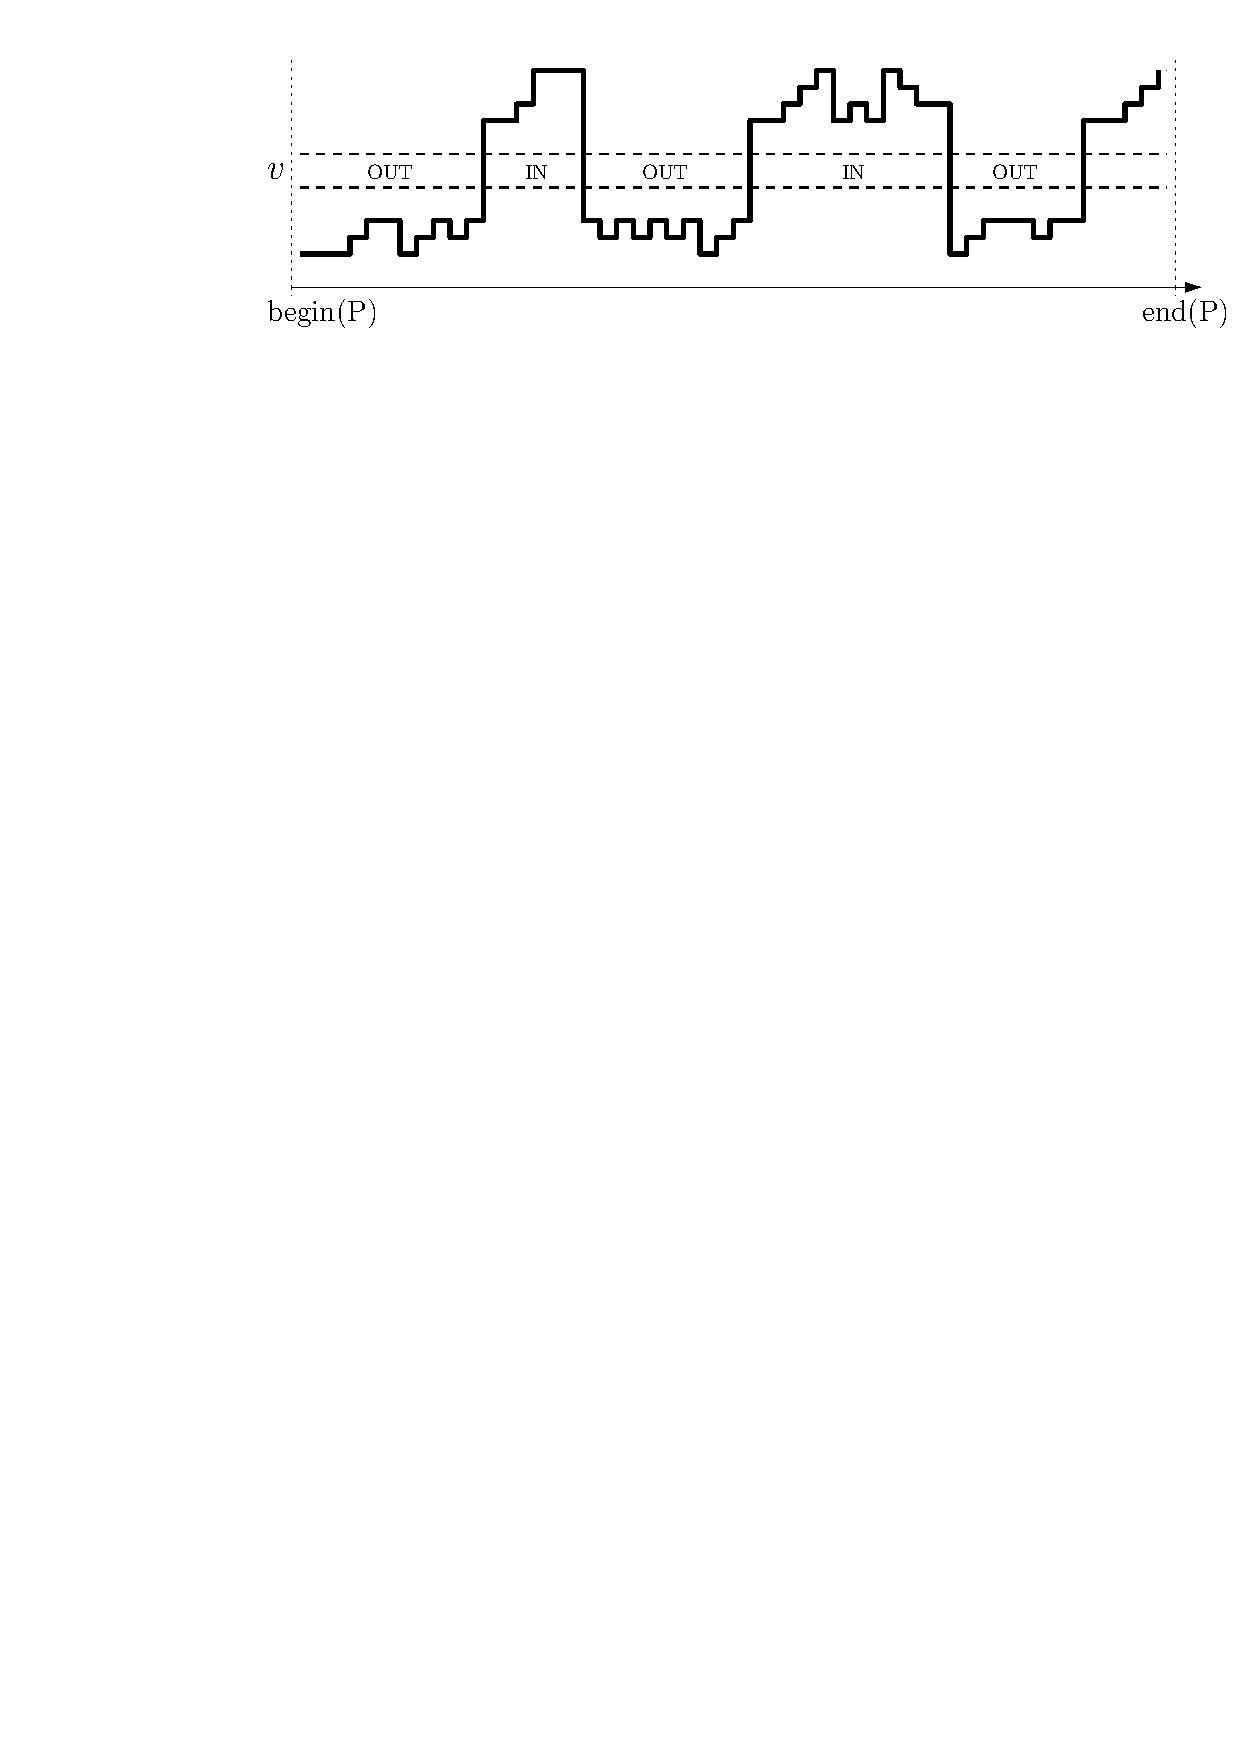
\includegraphics[width=0.9\columnwidth,keepaspectratio]{figs/cache-management/leftover}
\caption{Partitioning of the phase into interleaving \pin and \pout periods
for node $v$. The thick line represents cache contents. The \emph{leftover}
\pout period (the last one) is present for node $v$ as it has finished phase
$P$ inside \ALGTC's cache. The periods can be followed by requests contained in
$F^\infty$.}
\label{fig:leftover}
\end{figure}

We focus on a single node $v$.  We cut its history into interleaved periods:
\pout \emph{periods}, when $v$ is outside the cache and receives positive 
requests, and \pin \emph{periods} when \ALGTC keeps $v$ in the cache and $v$
receives negative requests. A final (possibly empty) part corresponding to the
time when $v$ is in the $F^\infty$ field is not accounted in \pout or \pin
periods, i.e., each \pin or \pout period corresponds to some field $F \in \F$.
Let $p^\pin$ and $p^\pout$ denote the total number of \pin and \pout periods
(respectively) for all nodes during the phase. An~example is given
in~\lref[Figure]{fig:leftover}.

Recall that \ALGTC starts each phase with an empty cache, and hence each node
starts with an \pout period. For $k_P$ nodes that are in {\ALGTC}'s cache at the
end of the phase (and only for them) their history ends with an \pout period
not followed by an \pin period. We call them \emph{leftover periods}. Thus,
$p^\pout = p^\pin + k_P$. The total number of periods ($p^\pin + p^\pout$) is
equal to the total size of all \emph{fields}, $\sizetc(\F)$, and thus $p^\pout 
\geq \sizetc(\F) / 2$.

We call a period \emph{full} if it has at least $\alpha/2$ requests. The
shifting strategies described in the previous section ensure that all
\pin periods are full and at least $1/(2 h(T))$ of all \pout periods are full.
Thus, there are at least $p^\pout/(2 h(T)) - k_P$ full non-leftover \pout
periods; each of them together with the following \pin period constitutes a
\emph{full \pout-\pin pair}.

\OPT has to pay at least $\alpha/2$ for the node in the course of the history
described by a~full \pout-\pin pair: it pays $\alpha$ either for changing the
cached/non-cached state of a node, or $\alpha/2$ for all positive requests or
$\alpha/2$ for all negative ones. Thus, $\OPT(P') \geq ( p^\pout / (2 h(T)) -
k_P ) \cdot \alpha/2 \geq ( \sizetc(\F) / (4 h(T)) - k_P ) \cdot \alpha/2$.
\end{proof}


%%%%%%%%%%%%%%%%%%%%%%%%%%%%%%%%%%%%%%%%%%%%%%%%%%%%%%%%%%%%%%%%%%%%%%%%%%%%%%%%%%%
%%%%%%%%%%%%%%%%%%%%%%%%%%%%%%%%%%%%%%%%%%%%%%%%%%%%%%%%%%%%%%%%%%%%%%%%%%%%%%%%%%%

\subsection{Competitive Ratio}
\label{sec:comp_ratio}

To relate the cost of \OPT to \ALGTC in a single phase $P$, we still need to
upper-bound $\req (F^\infty)$ and relate $k_P \cdot \alpha$ to the cost of
$\OPT$ (i.e., compare the bounds on \ALGTC and \OPT provided by
\lref[Lemma]{lem:alg_cost} and \lref[Lemma]{lem:leftovers}, respectively).

For the next two lemmas, we define $\VOPT$ as the set of all nodes that were
in \OPT cache at some time of~$P$ and let $\VOPTC = T \setminus \VOPT$. Note
that $\VOPT$ is a union of subforests (nodes present in \OPT's cache at
consecutive times), and hence a subforest itself.

\begin{lemma}
\label{lem:f_infty}
For any phase $P$, it holds that $\req (F^\infty) \leq 2 \cdot \kALG \cdot
\alpha + 2 \cdot \OPT(P)$.
\end{lemma}

\begin{proof}
We assume first that $P$ is a finished phase. Then, $P$ ends with an
artificial fetch of $X_{\enP}$ at time $\enP$ (followed by the final eviction).
We split $F^\infty$ into two disjoint parts (see \lref[Figure]{fig:fields}):
\begin{align*}
  F^\infty_- = &\; \{(v, t): v \in C_{\enP}, t \geq \last_v(\enP)\}, \\
  F^\infty_+ = &\; \{(v, t): v \notin C_{\enP} \sqcup X_{\enP}, \,
           t \geq \last_v(\enP)\}.
\end{align*}
Note that $F^\infty_-$ contains only negative requests and $F^\infty_+$ only
positive ones. As $\req(F^\infty) = \req(F^\infty_-) + \req (F^\infty_+ \cap
\VOPTC) + \req (F^\infty_+ \cap \VOPT)$, we estimate each of these summands
separately.
\begin{itemize}
\item
Nodes from $F^\infty_-$ are in the cache $C_{\enP}$ and were not
evicted from the cache. Thus, $\req(F^{\infty}_-) \leq |C_{\enP}| \cdot \alpha
\leq \kALG \cdot \alpha$.
\item
All the requests from $\VOPTC$ are paid by \OPT, and hence
$\req(F^\infty_+ \cap \VOPTC) \leq \req(\VOPTC) \leq \OPT(P)$.
\item
$F^\infty_+$ is a valid changeset for cache $C_{\enP} \sqcup X_{\enP}$.
As $\VOPT$ is a subforest of $T$, $F^\infty_+ \cap \VOPT$ is also a valid
changeset for the cache $C_{\enP} \sqcup X_{\enP}$. Therefore, $\req
(F^\infty_+ \cap \VOPT) \leq \sizetc(F^\infty_+ \cap \VOPT) \cdot \alpha$, as
otherwise the set fetched at time $\enP$ would not be maximal. (\ALGTC could
then fetch $X_{\enP} \sqcup (F^\infty_+ \cap \VOPT)$ instead of $X_{\enP}$.)
Thus, $\req (F^\infty_+ \cap \VOPT) \leq |\VOPT| \cdot \alpha = \kOPT \cdot
\alpha + (|\VOPT| - \kOPT)
\cdot \alpha \leq \kALG \cdot \alpha + \OPT(P)$.
The last inequality follows as --- independently of the initial state --- \OPT
needs to fetch at least $|\VOPT| - \kOPT$ nodes to the cache during $P$.
\end{itemize}
Hence, in total, $\req (F^\infty) \leq 2 \cdot \kALG \cdot
\alpha + 2 \cdot \OPT(P)$ for a finished phase $P$.

We note that if there was no cache change at $\enP$, the analysis above would
hold with $X_{\enP} = \emptyset$ with virtually no change. Therefore, for an
unfinished phase $P$ ending with a fetch or ending without cache change at
$\enP$, the bound on $\req(F^\infty)$ still holds. However, if an unfinished
phase~$P$ ends with an eviction, then we look at the last eviction-free 
time $\tau$ of~$P$. We now observe the evolution of field
$F^\infty$ from time~$\tau$ till $\enP$. At time $\tau$, $\req(F^\infty) \leq
2 \cdot \kALG \cdot \alpha + 2 \cdot \OPT(P)$. Furthermore, in subsequent
times, it may only decrease: at any round $F^\infty$ gets an additional
request, but on eviction $\req(F^\infty)$ decreases by $\alpha$ times
the number of evicted nodes (i.e., at least by $\alpha \geq 1$). Hence, the
value of $\req(F^\infty)$ at $\enP$ is also at most $2 \cdot \kALG \cdot
\alpha + 2 \cdot \OPT(P)$.
\end{proof}



By combining \lref[Lemma]{lem:alg_cost}, \lref[Lemma]{lem:leftovers} and 
\lref[Lemma]{lem:f_infty}, we immediately obtain the following corollary
(holding for both finished and unfinished phases).

\begin{corollary}
\label{cor:any_phase_bound}
For any phase $P$, it holds that 
$\ALGTC(P) \leq O(h(T)) \cdot \OPT(P) + O(h(T) \cdot (k_P + \kALG) \cdot \alpha)$.
\end{corollary}

Using the corollary above, its remains to bound the value of~$k_P$. This is
easy for an unfinished phase, as $k_P \leq \kALG$ there. For a~finished phase,
we provide another bound.

\begin{lemma}
\label{lem:opt_bound2}
For any finished phase $P$, it holds that
$k_P \cdot \alpha \leq \OPT(P) \cdot (\kALG + 1) / (\kALG + 1 - \kOPT)$.
\end{lemma}

\begin{proof}
First, we compute the number of positive requests in $\VOPTC$. Let $X_{t_1},
X_{t_2}, \ldots, X_{t_s}$ be all positive changesets applied by \ALGTC in~$P$.
For any~$t$, let $X'_t = X_t \setminus \VOPT$. As $X_t$ is some tree cap and
$\VOPT$ is a~subforest of $T$, $X'_t$ is a~tree cap of $X_t$. By
\lref[Corollary]{cor:density}, the number of requests to nodes of $X'_t$ in
field $F^t$ is at least $|X'_t| \cdot \alpha$. These requests for different
changesets $X_t$ are disjoint and they are all outside of $\VOPT$. Hence the
total number of positive requests outside of $\VOPT$ is at least $\sum_{i=1}^s
|X'_{t_i}| \cdot \alpha$, where $\sum_{i=1}^s |X'_{t_i}| \geq |\bigcup_{i=1}^s
X'_{t_i}| = |(\bigcup_{i=1}^s X_{t_i}) \setminus \VOPT| \geq |\bigcup_{i=1}^s
X_{t_i}| - |\VOPT| \geq k_P - |\VOPT|$.

Now $\OPT(P)$ can be split into the cost associated with nodes from $\VOPT$
and $\VOPTC$, respectively. For the former part,
\OPT has to pay at least $(|\VOPT| - \kOPT) \cdot \alpha$ for the fetches
alone. For the latter part, it has to pay $1$ for each of at least $(k_P -
|\VOPT|) \cdot \alpha$ positive requests outside of $\VOPT$. Hence, $\OPT(P)
\geq (|\VOPT| - \kOPT) \cdot \alpha + (k_P - |\VOPT|) \cdot \alpha = (k_P -
\kOPT) \cdot \alpha$. Then, $k_P \cdot \alpha \leq k_P \cdot \OPT(P) / (k_P -
\kOPT)$. As the phase is finished, $k_P \geq \kALG + 1$, and thus $k_P \cdot
\alpha \leq (\kALG + 1) \cdot \OPT(P) / (\kALG + 1 - \kOPT)$.
\end{proof}



\begin{theorem}
The algorithm \ALGTC is $O(h(T) \cdot \kALG/(\kALG-\kOPT+1))$-competitive.
\end{theorem}

\begin{proof}
Let $R = h(T) \cdot \kALG/(\kALG-\kOPT+1)$. We split an input~$I$ into a
sequence of finished phases followed by a single unfinished phase (which may
not be present). For a~finished phase $P$, we have $k_P > \kALG$, and hence
\lref[Corollary]{cor:any_phase_bound} and \lref[Lemma]{lem:opt_bound2}
imply that $\ALGTC(P) \leq O(R) \cdot \OPT(P)$. For an unfinished phase $k_P
\leq \kALG$, and therefore, by \lref[Corollary]{cor:any_phase_bound}, $\ALGTC(P)
\leq O(h(T)) \cdot \OPT(P) + O(h(T) \cdot \kALG \cdot \alpha)$. Summing over
all phases of $I$ yields $\ALGTC(I) \leq O(R) \cdot \OPT(I) + O(h(T) \cdot \kALG
\cdot \alpha)$.
\end{proof}

\subsection{No over-requested changesets}
\label{sec:proof_of_lemma_1}

Before proving \lref[Lemma]{lem:no_over-requested_changesets}, 
we present the following technical claim.


\begin{claim}
\label{cla:inductive_properties}
For any phase $P$, the following invariants hold for any time $t > \beP$:
\begin{enumerate}
\item $\cnt_{t-1}(X) < |X| \cdot \alpha$ for a valid changeset $X$ for $C_t$,\hspace{-1em}
\label{item:prop1}
\item $\cnt_t(X) \leq |X| \cdot \alpha$ for a valid changeset $X$ for $C_t$,
\label{item:prop2}
\item any changeset $X$ with property $\cnt_t(X) = |X| \cdot \alpha$ contains 
the node requested at round $t$.
\label{item:propmid}
\end{enumerate}
\end{claim}

\begin{proof}
First observe that \lref[Invariant]{item:prop1} (for time $t$) along with the
fact that round $t$ contains only one request immediately implies that
$\cnt_t(X) \leq \cnt_{t-1}(X) + 1 \leq (|X| \cdot \alpha - 1) + 1 = |X|
\cdot \alpha$, i.e., \lref[Invariant]{item:prop2} for time~$t$. Furthermore the equality may
hold only for changesets containing the node requested at round $t$, which
implies \lref[Invariant]{item:propmid} for time $t$.

It remains to show that \lref[Invariant]{item:prop1} holds for any step $t >
\beP$. It is trivially true for $t = \beP+1$ 
as $\cnt_{t-1}(X) = 0$ then. Let $t+1$ be the earliest time in phase $P$ for
which \lref[Invariant]{item:prop1} does not hold; we will then show a
contradiction with the definition of \ALG or a contradiction with other
Invariants at time $t$. That is, we assume that there exists a~positive
changeset $X$ for $C_{t+1}$ such that $\cnt_t(X) \geq |X| \cdot \alpha$ (the
proof for a negative changeset is analogous). Note that \ALG must have
performed an action (fetch or eviction) at time $t$ as otherwise $X$ would be
also  a changeset for $C_t = C_{t+1}$ with $\cnt_t(X) \geq |X| \cdot \alpha$,
which means that $X$ should have been applied by \ALG at time $t$. We consider
two cases.

If \ALG fetches a positive changeset $Y$ at time $t$, $C_{t+1} = C_t \sqcup Y$
and $\cnt_t(Y) = |Y|\cdot\alpha$. Then, $Y \sqcup X$ is a changeset for $C_t$,
and $\cnt_t(Y \sqcup X) \geq |Y \sqcup X| \cdot \alpha$. This contradicts
the maximality property of set~$Y$ chosen at time~$t$ by~\ALG.

If \ALG evicts a negative changeset $Y$ at time $t$, $C_{t+1} = C_t \setminus
Y$. \lref[Invariant]{item:prop2} and the definition of \ALG implies $\cnt_t(Y) =
|Y| \cdot \alpha$, and thus, by \lref[Invariant]{item:propmid}, $Y$ contains
the node requested at round $t$. As $X \cap Y \subseteq C_t$, \mbox{$X \cap Y$} does
not have any positive requests at time~$t$, and therefore $\cnt_t(X \setminus
Y) = \cnt_t(X) \geq |X| \cdot \alpha \geq |X \setminus Y| \cdot \alpha$. By
\lref[Invariant]{item:prop2}, $\cnt_t(X \setminus Y) \leq |X \setminus Y|
\cdot \alpha$, and hence $\cnt_t(X \setminus Y) = |X \setminus Y| \cdot
\alpha$. This contradicts \lref[Invariant]{item:propmid} as $X \setminus Y$
cannot contain the node requested at round $t$ (because $Y$ contains this
node).
\end{proof}


\begin{proof}[Proof of Lemma~\ref*{lem:no_over-requested_changesets}]
The inequality $\cnt_t(X) \leq |X| \cdot \alpha$ is equivalent to
\lref[Invariant]{item:prop2} of \lref[Claim]{cla:inductive_properties}.
Assume now that $X$ is applied at time $t$. By the definition of \ALG,
$\cnt_t(X) \geq |X| \cdot \alpha$, and thus $\cnt_t(X) = |X| \cdot \alpha$,
i.e., \lref[Property]{lemit:2} follows. Then, \lref[Invariant]{item:propmid}
of \lref[Claim]{cla:inductive_properties} implies \lref[Property]{lemit:1}.
Finally, \lref[Invariant]{item:prop1} of
\lref[Claim]{cla:inductive_properties} for time $t+1$ is equivalent to
\lref[Property]{lemit:3}.

To show \lref[Property]{lemit:4}, observe that the changeset $X$
applied at time $t$ cannot be a disjoint union of two (or more) valid
changesets $X_1$ and $X_2$. By \lref[Property]{lemit:2}, $|X| \cdot \alpha =
\cnt_t(X) = \cnt_t(X_1) + \cnt_t(X_2)$. If $\cnt_t(X_1) < |X_1| \cdot \alpha$
or $\cnt_t(X_2) < |X_2| \cdot \alpha$, then $\cnt_t(X_1) + \cnt_t(X_2) <
(|X_1| + |X_2|) \cdot \alpha = |X| \cdot \alpha$, a contradiction. Therefore,
$\cnt_t(X_1) = |X_1| \cdot \alpha$ and $\cnt_t(X_2) = |X_2| \cdot
\alpha$. But then \lref[Invariant]{item:propmid} of
\lref[Claim]{cla:inductive_properties} would imply that both $X_1$ and $X_2$
contain a node requested at time $t$, which is a~contradiction as they are
disjoint.

Therefore, if $X$ is a positive changeset applied at $t$, then $X$ is a~single
tree cap of a tree from subforest $C_{t+1}$, and likewise if $X$ is negative,
then $X$ is a~single tree cap of a~tree from subforest $C_t$.
\end{proof}
%%%%%%%%%%%%%%%%%%%%%%%%%%%%%%%%%%%%%%%%%%%%%%%%%%%%%%%%%%%%%%%%%%%%%%%%%%%%%%%%%%%
%%%%%%%%%%%%%%%%%%%%%%%%%%%%%%%%%%%%%%%%%%%%%%%%%%%%%%%%%%%%%%%%%%%%%%%%%%%%%%%%%%%

\section{Lower Bound on the Competitive Ratio}
\label{sec:lower-bound-on-the-problem}

\begin{theorem}
For any $\alpha \geq 1$, the competitive ratio of any deterministic online
algorithm for the online tree caching problem is at least
$\Omega(\kALG/(\kALG-\kOPT+1))$
\end{theorem}

\begin{proof}
We will assume that in the tree caching problem, evictions are free (this
changes the cost by at most by a factor of two). We consider a tree whose
leaves correspond to the set of all pages in the paging problem. The rest of
the tree will be irrelevant.

For any input sequence $I$ for the paging problem, we may create a sequence
$I_\textnormal{T}$ for tree caching, where a request to a page is replaced by
$\alpha$ requests to the corresponding leaf. Now, we claim that any solution
$A$ for~$I$ of cost $c$ can be transformed, in online manner, into a~solution
$A_\textnormal{T}$ for $I_\textnormal{T}$ of cost $\Theta(\alpha \cdot c)$ and
vice versa.

If upon a request $r$, an algorithm $A$ fetches $r$ to the cache and evicts
some pages, then $A_\textnormal{T}$ bypasses $\alpha$ corresponding requests
to leaf $r$, fetches $r$ afterwards and evicts the corresponding leaves,
paying $O(\alpha)$ times the cost of $A$. By doing it iteratively,
$A_\textnormal{T}$ ensures that its cache is equivalent to that of $A$. In
particular, a request free for $A$ is also free for $A_\textnormal{T}$.

Now take any algorithm $A_\textnormal{T}$ for $I_\textnormal{T}$. It can be
transformed to the algorithm $A_\textnormal{T}'$ that (i)~keeps only leaves of
the tree in the cache and (ii) performs actions only at times that are
multiplicities of $\alpha$ (losing at most a constant factor in comparison to
$A_\textnormal{T}$). Then, fix any chunk of $\alpha$ requests to some leaf
$r'$ immediately followed by some fetches and evictions of $A_\textnormal{T}'$
leaves. Upon seeing the corresponding request $r'$ in $I$, the algorithm $A$
performs fetches and evictions on the corresponding pages. In effect, the cost
of $A$ is $O(1/\alpha)$ times the cost of $A_\textnormal{T}$.

The bidirectional reduction described above preserves competitive ratios up to
a constant factor. Hence, applying the adversarial strategy for the paging
problem that enforces the competitive ratio  $R = \kALG/(\kALG-\kOPT+1)$
\cite{competitive-analysis} immediately implies the lower bound of $\Omega(R)$
on the competitive ratio for the tree caching problem.
\end{proof}




\section{Cache Updates with Fixed Cost}
\label{sec:bisimulation}


In this section, we present a formal argument showing why we can use any
$q$-competitive online algorithm $A_T$ for the tree caching problem to obtain
a $2 q$-competitive online algorithm~$A$ for the tree caching problem with updates with fixed cost $\alpha$.

Namely, we take any input $I$ for the latter problem and create, in online
fashion, an input $I_T$ for the tree caching problem.
For any solution for $I_T$, we may replay its actions (fetches and evictions)
on~$I$ and vice versa. However, there is one place, where these solutions 
may have different costs. Recall that an update of a~rule stored at node~$v$
in~$I$ is mapped to a \emph{chunk} of $\alpha$ negative requests to~$v$ 
in~$I_T$. It is then possible that an algorithm for $I_T$ modifies the cache
\emph{during} a chunk. An~algorithm that never performs such an action
is called \emph{canonical}.

To alleviate this issue, we first note that any algorithm $B$ for $I_T$ can be
transformed into a~canonical solution $B'$ by postponing all cache modifications
that occur during some chunk to the time right after it. Such a transformation
may increase the cost of a~solution on a~chunk at most by $\alpha$ and such an
increase occurs only when $B$ modifies a cache within this chunk. Hence, the
additional cost of transformation can be mapped to the already existing cost of
$B$, and thus the cost of $B'$ is at most by a factor of $2$ larger than that
of $B$.

Furthermore, note that there is a natural cost-pre\-serv\-ing bijection
between solutions to~$I$ and canonical solutions to~$I_T$ (solutions perform
same cache modifications). Hence, the algorithm $A$ for $I$ runs $A_T$
on~$I_T$, transforms it in an online manner into the canonical solution $A'_T(I_T)$, 
and replays its cache modification on $I$. Then, 
$A(I) = \; A'_T(I_T) \leq 2 \cdot A_T(I_T) 
\leq 2 q \cdot \OPT(I_T) \leq 2 q \cdot \OPT(I)$.

The second inequality follows immediately by the $q$-com\-pe\-ti\-ti\-ve\-ness
of $A_T$. The third inequality follows by replaying cache modifications as
well, but this time we take solution $\OPT(I)$ and replay its actions on $I_T$,
creating a canonical (not necessarily optimal) solution of the same cost.


%%%%%%%%%%%%%%%%%%%%%%%%%%%%%%%%%%%%%%%%%%%%%%%%%%%%%%%%%%%%%%%%%%%%%%%%%%%%%%%%%%%
%%%%%%%%%%%%%%%%%%%%%%%%%%%%%%%%%%%%%%%%%%%%%%%%%%%%%%%%%%%%%%%%%%%%%%%%%%%%%%%%%%%

\section{Implementation}\label{sec:implementing_counters}

The whole input fed to a tree caching algorithm is created at the
controller: positive requests are caused by cache misses (which redirect
packet to the controller) and batches of $\alpha$ negative requests are caused
by updates sent to the dynamic routing algorithm run at the controller.
Therefore, the whole tree caching algorithm can be implemented in software
in the controller only. The algorithm \ALGTC is a simple counter-based
scheme, and in this section we show that it can be implemented efficiently.


Recall that at each time $t$, \ALGTC verifies the existence of a valid changeset
that satisfies saturation and maximality properties (see the definition of
\ALGTC in \lref[Section]{sec:algo}). Here, we show that this operation can be
performed efficiently. In particular, in the following two subsections, we
will prove the following theorem.

\begin{theorem}
\ALGTC can be implemented using $O(|T|)$ additional memory, so that to make a~decision at time~$t$, it performs $O(h(T) + \max \{ h(T), \degree(T) \} \cdot |X_t|)$ operations,
where $\degree(T)$ is a~maximum node degree in $T$ and 
$X_t$ is the changeset applied at time $t$ ($|X_t| = 0$ if no changeset is
applied). 
\end{theorem}


Let $v_t$ be the node requested at round $t$. Note that we may restrict our
attention to requests that entail a~cost for \ALGTC, as otherwise its counters
remain unchanged and certainly \ALGTC does not change cache contents. We use
\lref[Lemma]{lem:no_over-requested_changesets} to restrict possible candidates
for changesets that can be applied at time $t$. First, we note that if a~node
$v_t$ requested at round $t$ is outside the cache, then, at time~$t$, \ALGTC may
only fetch some changeset, and otherwise it may only evict some changeset.
Therefore, we may construct two separate schemes, one governing fetches and
one for evictions.

In \lref[Section]{sec:implementing_positive_counters}, using 
\lref[Lemma]{lem:no_over-requested_changesets}, we show that after processing 
a~positive request, \ALGTC needs to verify at most $h(T)$ possible positive changesets,
each in constant time, using an auxiliary data
structure. The cost of updating this structure at time $t$ is 
$O(h(T) + h(T) \cdot |X_t|)$.

The situation for negative changesets is more complex as even after applying
\lref[Lemma]{lem:no_over-requested_changesets} there are still exponentially
many valid negative changesets to consider. In
\lref[Section]{sec:implementing_negative_counters}, we construct an~auxiliary
data structure that returns a viable candidate in time $O(h(T) + \degree(T)
\cdot |X_t|)$. The update of this structure at time $t$ can be also done in
$O(h(T) + \degree(T) \cdot |X_t|)$ operations.

\subsection{Positive Requests and Fetches}
\label{sec:implementing_positive_counters}

At any time $t$ and for any non-cached node $u$, we may define $P_t(u)$ as a
tree cap rooted at $u$ containing all non-cached nodes from $T(u)$. During an
execution of \ALGTC, we maintain two values for each non-cached node~$u$:
$\cnt_t(P_t(u))$ and $|P_t(u)|$. When a counter at node~$v_t$ is incremented, we
update $\cnt_t(P_t(u))$ for each ancestor~$u$ of~$v$ (at most $h(T)$ updated
values). Furthermore, if a node~$v$ changes its state from cached to
non-cached (or vice versa), we update the value of $|P_t(u)|$ for any ancestor $u$
of $v$ (at most $h(T)$ updates per each node that changes the
state). Therefore, the total cost of updating these structures at time $t$ is
at most $O(h(T) + h(T) \cdot |X_t|)$.

By \lref[Lemma]{lem:no_over-requested_changesets}, a positive valid changeset
fetched at time $t$ has to contain $v_t$ and is a single tree cap. Such a~tree
cap has to be equal to $P_t(u)$ for $u$ being an ancestor of $v_t$. 
Hence, we may iterate over all
ancestors $u$ of $v_t$, starting from the tree root and ending at $v_t$, and
we stop at the first node~$u$, for which $P_t(u)$ is saturated (i.e.,
$\cnt_t(P_t(u)) \geq |P_t(u)| \cdot \alpha$). If such a $u$ is found, the
corresponding set $P_t(u)$ satisfies also the maximality condition (cf.~the
definition of \ALGTC) as all valid changesets that are supersets of $P_t(u)$
were already verified to be non-saturated. Therefore, in such a case, \ALGTC
fetches~$P_t(u)$. Otherwise, if no saturated changeset is found, \ALGTC does
nothing. Checking all ancestors of $v_t$ can be performed in time $O(h(T))$.

\subsection{Negative Requests and Evictions}
\label{sec:implementing_negative_counters}

Handling evictions is more complex. If the request to
node $v_t$ at round $t$ was negative,
\lref[Lemma]{lem:no_over-requested_changesets} tells us only that the negative 
changeset evicted by \ALGTC has to be a tree cap rooted at $u$, where $u$ is the
root of the cached tree containing $v_t$. There are exponentially many such
tree caps, and hence their naïve verification is intractable. To alleviate
this problem, we introduce the following helper notion. For any set of cached
nodes~$A$ and any time $t$, let
\[
  \val_t(A) = \cnt_t(A) - |A| \cdot \alpha + \frac{|A|}{|T|+1}.
\]
Note that for any non-empty set $A$, $\val_t(A) \neq 0$ as the first two terms
are integers and $|A|/(|T|+1) \in (0,1)$. Furthermore, $\val_t$ is additive:
for two disjoint sets $A$ and $B$, $\val_t(A \sqcup B) =
\val_t(A) + \val_t(B)$. For any time~$t$ and a cached node $u$, we define
\begin{align*}
  H_t(u) = \arg \max_D \{ \val_t(D) : &\; \textnormal{$D$ is a non-empty tree cap} \\
    & \quad \textnormal{rooted at $u$} \}.
\end{align*}
Our scheme maintains the value $H_t(u)$ for any cached node $u$. To this end,
we observe that $H_t(u)$ can be defined recursively as follows. Let
$H'_t(u) = H_t(u)$ if $\val_t(H_t(u)) > 0$ and $H'_t(u) = \emptyset$ otherwise.
Then, for any node $v$ and time $t$, by the additivity of $\val_t$, 
\begin{equation*}
\label{eq:h_t_recurrence}
  H_t(u) = \{ u \} \; \sqcup \bigsqcup_\textnormal{$w$ is a child of $u$} H'_t(w).
\end{equation*}
Each cached node $u$ keeps the value $\val_t(H_t(u))$. Note that set $H_t(u)$
itself can be recovered from this information: we iterate over all children of
$u$ (at most $\deg(T)$ of them) and for each child $w$, if $\val_t(H_t(w)) >
0$, we recursively compute set $H_t(w)$. Thus, the total time for constructing
$H_t(u)$ is $O(\deg(T) \cdot |H_t(u)|)$.

During an execution of \ALGTC, we update stored values accordingly.
That is, whenever a~counter at a cached node $v_t$ is incremented, we update
$\val_t(H_t(u))$ values for each cached ancestor $u$ of $v_t$, starting from
\mbox{$u = v_t$} and proceeding towards the cached tree root. Any such update can be
performed in constant time, and the total time is thus $O(h(T))$. For a~cache
change, we process nodes from the changeset iteratively, starting with nodes
closest to the root in case of an~eviction and furthest from the root in case
of a fetch. For any such node $u$, we appropriately stop or start maintaining
the corresponding value of $\val_t(H_t(u))$. The latter requires looking up the
stored values at all its children. As $u$ does not have cached
ancestors, sets $H_t$ (and hence also the stored values) at other nodes 
remain unchanged. In total, the
cost of updating all $H_t$ values at time $t$ is at most $O(h(T) + \deg(T)
\cdot |X_t|)$.

Finally, we show how to use sets $H_t$ to quickly choose a~valid changeset for
eviction. Recall that for a negative request $v_t$, the changeset to be
evicted has to be a tree cap rooted at $u$, where $u$ is the root of a cached subtree
containing $v_t$. For succinctness, we use $H^u$ to denote $H_t(u)$. We show
that if $\val_t(H^u) < 0$, then there is no valid negative changeset that is
saturated, and hence \ALGTC does not perform any action, and if $\val_t(H^u) >
0$, then $H^u$ is both saturated and maximal, and hence \ALGTC may evict~$H^u$.

\begin{enumerate} 
\item First, assume that $\val_t(H^u) < 0$. Then, for any tree cap~$X$ rooted
at~$u$, it holds that $\cnt_t(X) - |X| \cdot \alpha < \val_t(X) \leq
\val_t(H^u) < 0$, i.e., $X$ is not saturated, and hence cannot be evicted by
\ALGTC.

\item Second, assume that $\val_t(H^u) > 0$. As $\cnt_t(H^u) - |H^u| \cdot
\alpha$ is an integer and $|H^u|/(|T|+1) < 1$, it holds that $\cnt_t(H^u) -
|H^u| \cdot \alpha \geq 0$, i.e., $H^u$ is saturated. Moreover, by
\lref[Lemma]{lem:no_over-requested_changesets}, $\cnt_t(H^u) \leq |H^u| \cdot
\alpha$, and therefore $\cnt_t(H^u) - |H^u| \cdot \alpha = 0$, i.e.,
$\val_t(H^u) = |H^u| / (|T|+1)$. It remains to show that $H^u$ is maximal,
i.e., there is no valid saturated changeset $Y \supsetneq H^u$. By
\lref[Lemma]{lem:no_over-requested_changesets}, $Y$ has to be a tree cap
rooted at $u$ as well. If $Y$ was saturated, $\val_t(Y) = \cnt_t(Y) - |Y|
\cdot \alpha + |Y| / (|T|+1) \geq |Y| / (|T|+1) > |H^u|/(|T|+1) = \val_t(H^u)$, 
which would contradict the definition of~$H^u$.
\end{enumerate}

Note that node $u$ can be found in time $O(h(T))$, and the 
actual set~$H^u$ (of size $|X_t|$) can be computed 
in time $O(\deg(T) \cdot |X_t|)$. Therefore the total time 
for finding set $|X_t|$ is $O(h(T) + \deg(T) \cdot |X_t|)$.


%\subsection{Practical Considerations}
%
%In practical implementations, one may also resort to standard techniques such
%as sampling. Namely, for each request that costs $1$ (that would normally
%entail counter updates), we toss a biased coin. Then, we ignore this request in
%counter updates with probability $(1-1/\sqrt{\alpha})$ and we increment a
%corresponding counter by $\sqrt{\alpha}$ with probability $1/\sqrt{\alpha}$.
%This modification can tremendously speed up the execution of the algorithm,
%while sacrificing the (expected) competitive ratio only by a constant factor.
%Details will be given in the full version of the paper.
%\end{comment}

%%%%%%%%%%%%%%%%%%%%%%%%%%%%%%%%%%%%%%%%%%%%%%%%%%%%%%%%%%%%%%%%%%%%%%%%%%%%%%%%%%%
%%%%%%%%%%%%%%%%%%%%%%%%%%%%%%%%%%%%%%%%%%%%%%%%%%%%%%%%%%%%%%%%%%%%%%%%%%%%%%%%%%%


\section{Conclusions}\label{sec:conclusion-caching}

In this chapter we define a novel variant of online paging which finds
applications in the context of IP routing networks where forwarding rules can
be cached. We presented a deterministic online algorithm that achieves a
provably competitive trade-off between the benefit of caching and update costs.

It is worth noting that, in the offline setting, choosing the best static cache 
in the presence of only positive requests is known as a~\emph{tree sparsity}
problem and can be solved in $O(|T|^2)$ time~\cite{tree-sparsity}.

We believe that our work opens interesting directions for future research.
Most importantly, it will be interesting to study the optimality of the
derived result; we conjecture that the true competitive ratio does not 
depend on the tree height. In particular, primal-dual approaches that were
successfully applied for other caching
problems~\cite{young-paging-greedy-dual,generalized-caching-optimal,generalized-caching-bansal} may turn out to be useful also for the considered variant. 


%%%%%%%%%%%%%%%%%%%%%%%%%%%%%%%%%%%%%%%%%%%%%%%%%%%%%%%%%%%%%%%%%%%%%%%%%%%%%%%%%
%%%%%%%%%%%%%%%%%%%%%%%%%%%%%%%%%%%%%%%%%%%%%%%%%%%%%%%%%%%%%%%%%%%%%%%%%%%%%%%%%


\chapter{Summary and outlook}
Does not belong to any part of the thesis, or rather to both of them.


\chapter{Appendix}

\appendix

From file appendix.tex

\bibliographystyle{plain}
\bibliography{references}

\end{document}
